% !TeX spellcheck = en_US
% !TeX encoding = UTF-8
% !TeX program = xelatex

%\PassOptionsToPackage{unicode}{hyperref}
%\PassOptionsToPackage{naturalnames}{hyperref}

\documentclass[lang=cn,newtx,10pt,scheme=chinese,device=pad]{elegantbook}

\title{数学笔记}
\subtitle{偏微分方程--趋化模型}

\author{毛宣}
\institute{东南大学数学学院}
\date{2024/06/11}
\version{0.1.0}
\bioinfo{测试}{信息}

\extrainfo{注意:本模板自 2023 年 1 月 1 日开始,不再更新和维护!}

\setcounter{tocdepth}{3}

\logo{logo-blue.png}
\cover{cover.jpg}

% 本文档命令
\usepackage{array}
\newcommand{\ccr}[1]{\makecell{{\color{#1}\rule{1cm}{1cm}}}}


% 修改标题页的橙色带
\definecolor{customcolor}{RGB}{32,178,170}
\colorlet{coverlinecolor}{customcolor}
\usepackage{cprotect}

\usepackage{mathtools} %provided \shortintertext

\addbibresource[location=local]{mynote.bib} % 参考文献,不要删除

\allowdisplaybreaks[4]

\includeonly{mathnote,real-analysis}
%\includeonly{functional-analysis}

\newcommand{\set}[1]{\left\{#1\right\}}

\newcommand{\Lref}[1]{Lemma~\ref{#1}}

\newcommand{\dd}{\;\mathrm{d}}

\DeclareMathOperator*{\esssup}{ess\,sup}

\begin{document}

\maketitle
\frontmatter

\tableofcontents

\mainmatter

%\part{mathematics analysis}
\chapter{数学分析}


%-=-=-=-=-=-=-=-=-=-=-=-=-=-=-=-=-=-=-=-=-=-=-=-=
%	SECTION:
%-=-=-=-=-=-=-=-=-=-=-=-=-=-=-=-=-=-=-=-=-=-=-=-=

\section{集合与映射}\index{Set ! function}

\begin{example}\label{20151012-190708}
\hfill \\
设$f(x)$对任意的$x\in R$有$f(x)=f(x^2)$,且$f(x)$在$x=0$和$x=1$ 处连续。证明$f(x)$在$R$上为常数。(上海交通大学,2003)


steps
  $f(x)$在$x=0$处连续$\Leftrightarrow\forall\varepsilon>0,\exists\delta>0,\forall x\in(-\delta,\delta),|f(x)-f(0)|<\varepsilon$。
  
  $\forall x\in(-1,1),|f(x)-f(0)|=|f(x^2)-f(0)|\cdots=|f(x^{2n}-f(0)|$
  即对上述的$\varepsilon>0$,$\exists N=\max\{1,[\log_x\frac{\delta}2]\}$,$\forall n>N,x^{2n}<\delta$,从而$|f(x)-f(0)|=|f(x^{2n}-f(0)|<\varepsilon$成立。
  
  由$\varepsilon$的任意性,有$\forall x\in(-1,1),f(x)\equiv f(0).(|f(x)-f(0)|\leq 0)$
  
  又$f(x)$在$x=1$处连续$\Leftrightarrow\forall\varepsilon>0,\exists\delta>0,\forall x\in(1-\delta,1+\delta),|f(x)-f(1)|<\varepsilon$成立。
  而$\forall x>1,|f(x)-f(1)|=|f(x^{\frac12})-f(1)|=\cdots|f(x^{\frac1{2n}})-f(1)|$,
  即对上述的$\varepsilon>0,\exists N=\max\{1,[\frac1{2\log_x(1+\delta)}]\},\forall n>N,0<x^{\frac 1{2n}}-1<1+\delta,|f(x)-f(1)|=|f(x^{\frac1{2n}})-f(1)|<\varepsilon$。
  
  由$\varepsilon$的任意性,$0\leq|f(x)-f(1)|\leq 0$,从而$\forall x>1,f(x)\equiv f(1)$。
  
  易知$\forall x<-1,f(x)=f(x^2)=f(1)$,又$f(0)=\lim_{x\rightarrow1^-}f(x)=f(1)=f(-1)$,从而$\forall x\in R,f(x)\equiv f(0)$。

%\qdepend

%\qdependlist
\end{example}
\hfill\\

\section{数列极限}
  \begin{example}
  \hfill\\
   Cauchy收敛准则,叙述并证明。(浙江大学,2003)

  Cauchy收敛准则:数列$\{a_n\}$收敛的充分必要条件是$$\forall\varepsilon>0,\exists N,\forall m,n>N,|a_m-a_n|<\varepsilon.$$
  
  必要性:数列$\{a_n\}$收敛,则$\exists a$使得$\forall\varepsilon>0,\exists N,\forall n>N$,有
  $|a_n-a|<\frac{\varepsilon}2$,从而$\forall m,n>N,|a_m-a_n|\leq|a_m-a|+|a_n-a|<\varepsilon.$
  
  充分性:若$\forall\varepsilon>0,\exists N,\forall m,n>N,|a_m-a_n|<\varepsilon.$则当$\varepsilon=1$时,$\exists N_1$,固定$m+N_1+1,\forall n>N_1,|a_n-a_m|<\varepsilon$。从而数列
  $\{a_n\}$必有界,由抽子列定理,存在子列$\{a_{n_j}\}$收敛到$a$。
  
  于是$\forall\varepsilon>0,\exists N_2,\forall n_j>N_2,|a_{n_j}-a|<\varepsilon.$
  
  $|a_n-a|=|a_n-a_{n_j}+a_{n_j}-a|\leq|a_n-a_{n_j}|+|a_{n_j}-a|\leq\varepsilon+\varepsilon=2\varepsilon.$
  故$\{a_n\}$收敛。

\end{example}

\begin{example}
\hfill\\

 任意给定$x\in R$,令$x_1=\cos x,x_{n+1}=\cos x_n$,证明数列收敛。
 

  $\because x_1\in[-1,1],\therefore x_2\in[-1,1]$归纳易知,$\forall n\in N^+,0\leq|x_n|\leq1$又
  \[
  \begin{aligned}
  |x_{n+1}-x_n|&=|\cos x_n-\cos x_{n-1}|\\
  &=2|\sin^2\frac{x_n}2-\sin^2\frac{x_{n-1}}2|\\
  &=2|\sin\frac{x_n}2-\sin\frac{x_{n-1}}2||\sin\frac{x_n}2+\sin\frac{x_{n-1}}2|\\
  &\leq2|\sin\frac{x_n}2-\sin\frac{x_{n-1}}2|(|\sin\frac{x_n}2|+|\sin\frac{x_{n-1}}2|)\\
  &<2|\sin\frac{x_n}2-\sin\frac{x_{n-1}}2|(\sin\frac12+\sin\frac12)\\
  &=2|\sin\frac{x_n}2-\sin\frac{x_{n-1}}2|\cdot\delta,\verb+其中+\delta=2\sin\frac12\in(0,1)
  \end{aligned}
\]
由拉格朗日中值定理可证:$|\sin\frac{x_n}2-\sin\frac{x_{n-1}}2|\leq\frac12|x_n-x_{n-1}|$。于是$|x_{n+1}-x_n|<\delta|x_n-x_{n-1}|$其中$\delta\in(0,1)$。易推:$|x_{n+1}-x_n|<\delta^n|x_1-x|$于是对$0<n<m$有
\[
\begin{aligned}
|x_m-x_n|&=|x_m-x_{m-1}+x_{m-1}\cdots+x_{n+1}-x_n|\\
&\leq\sum_{i=n+1}^m|x_i-x_{i-1}|\\
&<|x_1-x|\sum_{i=n+1}^m\delta^{i-1}\\
&=|x_1-x|\frac{\delta^n(1-\delta^{m-n}}{1-\delta}\\
&<|x_1-x|\frac{\delta^n}{1-\delta}\rightarrow0,n\rightarrow\infty.
\end{aligned}
\]
即$\forall\epsilon>0,\exists N\in N^+,\forall m,n>N,\verb+有+|x_m-x_n|<\epsilon$,由Cauchy收敛准则知:$\{x_n\}$收敛。

\end{example}
\begin{example}
\hfill\\
设$\phi(x)$与$f(x)$是区间$[a,b]$上的正值连续函数,求证:$$\displaystyle\lim_{n\rightarrow\infty}\frac{\int_a^b\phi(x)f^{n+1}(x)dx}{\int_a^b\phi(x)f^n(x)dx}=\max_{a\leq x\leq b}f(x).$$

设$I_n=\int_a^b\phi(x)f^n(x)\mathrm{d}x$。应用Schwarz不等式,得
$$I_n^2\leq\int_a^b\phi(x)f^{n-1}(x)\mathrm{d}x\int_a^b\phi(x)f^{n+1}(x)\mathrm{d}x=I_{n-1}I_{n+1}.$$
故$$\frac{I_{n+1}}{I_n}\geq\frac{I_n}{I_{n-1}}.$$
因此数列$\{\frac{I_{n+1}}{I_n}\}$是递增的,又
$$\frac{I_{n+1}}{I_n}\leq\max_{a\leq x\leq b}f(x)\frac{I_n}{I_n}=\max_{a\leq x\leq b}f(x),$$
所以$\{\frac{I_{n+1}}{I_n}\}$有界。于是$\lim_{n\rightarrow\infty}\frac{I_{n+1}}{I_n}$存在,且
$$\lim_{n\rightarrow\infty}\frac{I_{n+1}}{I_n}=\lim_{n\rightarrow\infty}\sqrt[n]{I_n}.$$
而$$\lim_{n\rightarrow\infty}\sqrt[n]{I_n}=\max_{a\leq x\leq b}f(x).$$
这就完成了证明。
\end{example}

\begin{example}
\hfill\\
试证$\sum1/p$发散,其中$p$遍历一切质数。

提示:给定$N$,设$p_1,p_2,\cdots,p_k$是至少能整除一个不大于$N$的正整数。那么$$\sum_{n=1}^N\frac{1}{n}\leq\prod_{i=1}^k(1+\frac{1}{p_i}+\frac{1}{p_i^2}+\cdots)=\prod^k(1-\frac{1}{p_i})^{-1}\leq\exp\sum_{i=1}^k\frac{2}{p_i}.$$
最后这个不等式能成立,是因为当$0\leq x\leq \frac{1}{2}$时,$(1-x)^{-1}\leq e^{2x}$。显然当$N\rightarrow+\infty$时,$k\to\infty$,从而
$$\lim_{N\to\infty}\exp\sum_{i=1}^{N(k)}\frac{2}{p_i}\geq\lim_{n\to\infty}\sum_{n=1}^N\frac{1}{n}=+\infty.$$
于是$\sum\frac{2}{p_i}\to\infty$,$k\to\infty$。得证。
\end{example}
\hfill\\
  \section{函数极限与连续函数}
  \begin{example}
  \hfill\\
  
  若函数$f(x)$在$[0,+\infty)$上连续,$\displaystyle\lim_{x\rightarrow\infty}f(x)=A$存在,则$f(x)$在$[0,+\infty)$上一致连续。(中国人民大学,2001)
 
  $\lim_{x\rightarrow\infty}f(x)=A\Leftrightarrow$对任意的$\varepsilon>0,\exists M>0,\forall x_1,x_2>M,|f(x_1)-f(x_2)|<\varepsilon$。
  
  因为$f(x)$在$[0,M+1]$上连续,从而在$[0,M+1]$上一致连续,即存在$0<\delta<1$,对任意的$x_1,x_2\in[0,M+1]$,当$|x_1-x_2|<\delta$时,有$|f(x_1)-f(x_2)|<\varepsilon$。因此,对任意的$x_1,x_2\in[0,+\infty)$,当$|x_1-x_2|<\delta$时,有$|f(x_1)-f(x_2)|<\varepsilon$。
  
  即$f(x)$在$[0,+\infty)|<\varepsilon$。
  \end{example}
  \begin{example}
  \hfill\\
  证明:函数$f(x)=\sqrt{x}lnx$在$[1,+\infty)$上一致连续。(北京大学,2001)
  
  steps
  对$f(x)$求导可得
  \[f'(x)=\frac{\ln x+2}{2\sqrt x},\]
  \[f''(x)=-\frac{\ln x}{4x\sqrt x.}\]
  当$x\in[1,+\infty)$时,$f'(x)>0,f''(x)<0$,因此,$f'(x)$在$[1,+\infty)$上单调递减趋于0,又$\lim_{x\rightarrow1}f'(x)=1$,意味着$f'(x)$在$[1,+\infty)$有界,不妨假设$|f'(x)|\leq M$。
  
  对任意的$\varepsilon>0,\exists\delta=\frac{\delta}M,$对任意的$x_1,x_2\in[1,+\infty)$,当$|x_1,x_2|<\delta$时,有$|f(x_1)-f(x_2)|=|f'(\xi)(x_1-x_2)|<M\cdot\frac{\varepsilon}{M}=\varepsilon.$其中$\xi\in[x_1,x_2]$,即函数$f(x)=\sqrt{x}\ln x$在$[1,+\infty)$上一致收敛。
  \end{example}

\begin{remark}
  札记:可以用Cauchy收敛准则和微分中值定理证明函数一致连续性
\end{remark}

\begin{example}
\hfill\\
  设$f(x)$在$[a,b]$上连续,对$x\in[a,b]$定义$\displaystyle m(x)=\inf_{a\leq t\leq x}f(t)$。证明:$m(x)$在$[a,b]$上连续。(大连理工大学,2004)
  
  
  首先,因为闭区间上的连续函数必有最大值和最小值,故$m(x)$是良定义的。
  
  其次,$\forall a\leq x_1<x_2\leq b$,
  \[
  \begin{aligned}
  m(x_2)&=\inf_{a\leq t\leq x_1}f(t)\\
  &=\min\{\inf_{a\leq t\leq x_1}f(t)+\inf_{x_1\leq t\leq x_2}f(t)\}\\
  &\leq\min_{a\leq t\leq x_1}f(t)\\
  &=m(x_1)\\
  \end{aligned}
  \]
  故$m(x)$在$[a,b]$上单调递减,$\forall x_1,x_2\in[a,b],|x_1-x_2|<2\delta$,因为$f(x)$在$[a,b]$上一致连续,故$\forall\varepsilon>0,\exists\delta<0,|f(x_1)-f(x_2)|<\varepsilon.$从而$\forall x\in[a,b]$,
  \[
  \begin{aligned}
  m(x+)&=\lim_{\delta\rightarrow0+}m(x+\delta)\\
  &=\lim_{\delta\rightarrow0+}\frac{m(x)+\inf_{x\leq t\leq x+\delta}f(t)-|m(x)-\inf_{x\leq t\leq x+\delta}f(\delta)|}{2}\\
  &=\frac{m(x)+f(x)-|f(x)-m(x)|}{2}\\
  &=m(x)\\
  \end{aligned}
  \]
  对$m(x-)$,若$m(x)<m(x-\delta)$,则$f(\eta)=m(x)\leq m(x-\delta)\leq f(x-\delta),(\eta\in(x-\delta,x))$
  因为$f(x)$在$[a,b]$上一致连续,故$\forall\varepsilon>0,\exists\delta>0,x_1,x_2\in[a,b],|x_1-x_2|<\delta,|f(x_1)-f(x_2)|<\varepsilon$。从而对上述$\varepsilon>0$,有上述$\delta>0$,$$|m(x)-m(x-\delta)|\leq|f(\eta)-f(x-\delta)|<\varepsilon,(\eta\in(x-\delta,x).$$
  由此$m(x)$在$x$处左连续,右连续。故$m(x)$在$[a,b]$上连续。
  \end{example}
  
  \begin{example}
  \hfill\\
  如果$f$是$(0,\infty)$上的正值函数,合于
  \begin{enumerate}
  \item[a] $f(x+1)=xf(x)$;
  \item[b] $f(1)=1$;
  \item[c] $\log f$是凸的;
  \end{enumerate}
  那么$f(x)=\Gamma(x)$。其中$$\Gamma(x)=\int_0^{\infty}t^{x-1}e^{-t}\mathrm{d}t.$$
  
  因为$\Gamma$函数满足以上三点,那么只需证明$x>0$时$f(x)$是由以上三点决定的函数就行了。根据$a$只需考虑$x\in(0,1).$
  
  令$\varphi =\log f$,那么$\varphi(x+1)=\varphi(x)+\log x(0<x<\infty).$ $\varphi(1)=0$,并且$\varphi$是凸的,假定$0<x<1$,而$n$是正整数,由上式$\varphi(n+1)=\log (n!).$现在考虑一下$\varphi$在$[n,n+1]$,$[n+1,n+1+x]$,$[n+1,n+2]$三个区间上的差商,既然$\varphi$是凸的,那么$$\log n\leq\frac{\varphi(n+1+x)-\varphi(n+1)}{x}\leq\log(n+1).$$
  $$\varphi(n+1+x)=\varphi(x)+\log[x(x+1)\cdots(x+n)].$$
  所以$$0\leq\varphi(x)-\log[\frac{n!n^x}{x(n+1)\cdots(x+n)}]\leq x\log(1+\frac{1}{n}).$$
  最末的式子当$n\to\infty$时趋于零。从而确定了$\varphi$。
  \end{example}
 
\begin{example}
\hfill\\
定义区间$(a,b)$上的实连续函数满足:
$$\forall x,y \in(a,b),f(\frac{x+y}{2})\leq\frac{1}{2}(f(x)+f(y)).$$
求证:$f$是凸函数。其中,所谓凸函数是指
$$f(\lambda x+(1-\lambda)y)\leq\lambda f(x)+(1-\lambda)f(y),\forall x,y\in(a,b),\lambda\in(0,1).$$

\textbf{引理:}若非空集合$S\subset(0,1)\cap\mathit{Q}$满足:若$\frac{1}{2}\in S$;若$p\in S$,则$\frac{p}{1+p},\frac{1}{1+p}\in S.$则$S=(0,1)\cap\mathit{Q}$。

引理的证明只需注意到,$(0,1)$的有理数可用真分数表示,而全体真分数具有$\frac{q}{p}$形式,其中$p<q\in\mathrm{N}^*$。于是我们可以关于分母$p=N$作第二数学归纳法证明上述引理。

我们想用上述引理说明,当$\lambda\in S$时,凸函数定义中的不等式成立。又因为$S$在$(0,1)$中稠密,以及$f$的连续性,可以说明$\forall\lambda\in(0,1)$,凸函数定义中的不等式成立。从而证毕。

现在我们只需说明,若$p\in S$,则$\frac{p}{1+p},\frac{1}{1+p}\in S$即可。

\begin{align*}
f(\frac{p}{1+p}x+\frac{1}{p+1}y)&=f(p(\frac{1}{1+p}x+\frac{p}{1+p}y)+(1-p)y)\\
&\leq pf(\frac{1}{1+p}x+\frac{p}{1+p}y)+(1-p)f(y)\\
&\leq p^2f(\frac{p}{1+p}x+\frac{1}{p+1}y)+p(1-p)f(x)+(1-p)f(y)\\
\end{align*}
于是
$$f(\frac{p}{1+p}x+\frac{1}{p+1}y)\leq \frac{p}{1+p}f(x)+\frac{1}{p+1}f(y),$$
即$\frac{p}{1+p},\frac{1}{1+p}\in S.$证毕。
\end{example} 
 
  \hfill\\



\section{微分}
  \begin{example}
  \hfill\\
   已知$f(x)$可导,$f(x)+f'(x)\rightarrow a,x\rightarrow+\infty$,则$x\rightarrow+\infty$有$f(x)\rightarrow a,f'(x)\rightarrow0$。(清华大学,2006)
  
  反设$f(x)\nrightarrow a$。
  
  若$f(x)\rightarrow+\infty,x\rightarrow+\infty\Leftrightarrow\forall M>0,\exists N,\forall x>N,f(x)>M.$
  
  即对$x_0,\exists x_1>x_0+1,f(x_1)>f(x_0)$;
  
  $\exists x_2>x_1+1,f(x_2)>f(x_1)$;于是有一列$\{x_n\}$满足$x_{n+1}>x_n+1$,且$f(x_{n+1})>f(x_n)$,从而$x_n\rightarrow\infty$,且$f(x_n)\rightarrow+\infty$。
  
  由微分中值定理,存在一列$\{\xi_n\}$,有$f'(\xi_n)>0$,其中$$\xi_n\in[x_{n-1},x_n],n=1,2,\cdots$$,这与$f'(x)\rightarrow+\infty$矛盾,故$$f(x)\nrightarrow+\infty,x\rightarrow+\infty$$。
  
  同理,$f(x)\nrightarrow-\infty,x\rightarrow+\infty$,从而$f(x)$有界。
  
  于是$f(x)$
  
  证明有问题。
  \end{example}
  \begin{example}
  \hfill\\
   设$f(x)$,$g(x)$在$[a,b]$上连续,$(a,b)$内可导,$g'(x)\neq0$。证明:$\exists\xi\in(a,b)$,使$\frac{f(a)-f(\xi)}{g(\xi)-g(b)}=\frac{f'(\xi)}{g(\xi)}$(武汉大学,2004)
  
  记$F(x)=f(a)g(x)+g(b)f(x)-f(x)g(x)$,
  则$F(x)$在$[a,b]$上连续,在$(a,b)$内可导,又$F(a)=f(a)g(b)=F(b)$,从而由Largange中值定理:
  $\exists\xi\in(a,b),$$$\frac{F(a)-F(b)}{a-b}=F'(\xi)=0$$,即$$f(a)g'(\xi)+g(b)f'(\xi)-f'(\xi)g(\xi)-f(\xi)g'(\xi)=0.$$
  
  即$\frac{f(a)-f(\xi)}{g(\xi)-g(b)}=\frac{f'(\xi)}{g'(\xi)}$。
  
  考虑到$g'(x)\neq 0,$从而$g(\xi)\neq g(b)$,因为不然,若$g(\xi)=g(b),\xi\in(a,b)$,由微分中值定理,$\exists\eta\in(\xi,b),g'(\eta)=0$与$g'(x)\neq0$矛盾,故上式是有意义的。
  \end{example}
  \begin{example}
  \hfill\\
   设$f(x)$在$(a,b)$上可微,$f'(x)$在$(a,b)$上单调。求证:$f'(x)$在$(a,b)$上连续。(北京航空航天大学,2004)
  
  不妨设$f(x)$单调递增,从而$\forall c\in(a,b)$,$f'(x)$在$(a,c)$上单调递增有上界,$f(x)\leq f(c)$。由确界原理,$\exists S_c=\sup_{x\in(a,c)}f'(x)$,由确界定义与左极限定义易知:$f(c-)=S_c$。同理$f(c+)=I_c=\inf_{x\in(c,b)}f'(x)$。
  故单调的导函数不存在第二类间断点。
  
  又$f'(c-)\leq f'(c+)$,由达布引理,导函数具有介值性,若$f'(c-)<f'(c+)$,$\forall\eta\in[f'(c-),f'(c+)],\exists\xi\in[c-\varepsilon,c+\varepsilon],f'(\xi)=\eta.$而这样的$\xi$时不存在的,因为$f'(x)$单调。从而$f'(c-)=f'(c+)$,即导函数连续。
  \end{example}
  \begin{exercise}
  \hfill\\
 设$f(x)$在$[a,b](a<b)$上处处有正的二阶导数,证明存在常数$0<m\leq M$,使$\frac m4(x-a)^2\leq f(x)-2f(\frac{x+a}2)+f(a)\leq \frac M4(x-a)^2,x\in(a,b]$。(南京航空航天大学,2003) 
  
  设$$F(x)=
  \begin{cases}
  \frac{f(x)-2f(\frac{x+a}{2})+f(a)}{(x-a)^2},&x>a,\\
  \frac{f''(a)}{4},&x=a,\\
  \end{cases}
  $$
  则
  \begin{align*}
  F(a+)&=\lim_{x\rightarrow a+}\frac{f(x)-2f(\frac{x+a}{2})+f(a)}{(x-a)^2}\\
  &=\lim_{x\rightarrow a+}\frac{f'(x)-f'(\frac{x+a}{2}}{2(x-a)}\\
  &=\lim_{x\rightarrow a+}\frac{f''(x)}{2}-\frac{f''(\frac{x+a}{2})}{4}\\
  &=\frac{f''(a)}{4}\\
  &=F(a),\\
  \end{align*}
  从而$F(x)$在$[a,b]$上连续。
  
  下面证明$F(x)$在$[a,b]$上恒正。
 因为
 \begin{align*}
 &f(x)-2f(\frac{x+a}{2})+f(a)\\
 &=f'(\xi)(x-\frac{x+a}{2})-f'(\eta)(\frac{x+a}{2}-a)\\
 &=[f'(\xi)-f'(\eta)]\frac{x-a}{2}\\
 &=\frac{f''(\phi)}2(x-a)(\xi-\eta)\quad(x>a),\\
 \end{align*}
 其中$\xi\in(\frac{x+a}{2},x)$,$\eta\in(a,\frac{x+a}{2})$,$\phi\in(\eta,\xi)$,又$f''(x)$在$[a,b]$上恒正。
 故$F(x)$在$[a,b]$上恒正。$F(x)$在$[a,b]$上连续故闭存在最大值$\frac{M}{4}$和最小值$\frac{m}{4}$。这就完成了证明。  
  \end{exercise}  
  
  \hfill\\

  \section{微分中值定理及其应用}
  \begin{example}
  \hfill\\
  设$f(x)\in[0,1]$上可导,$f(1)=2\int xf(x)dx$。求证:存在$\xi\in(0,1)$,使得$f'(\xi)=-\frac{f(\xi)}{\xi}$。(清华大学,2003)
  
  
  反设$\forall\xi\in(0,1),f'(\xi)+\frac{f(\xi)}{\xi}=\frac{\xi f'(\xi)+f(\xi)}{\xi}=0$均不成立。
  
  从而$\xi f'(\xi)+f(\xi)$恒正或恒负(Darboux引理,导函数介值性)。不妨设
  $$\forall\xi\in(0,1),\xi f'(\xi)+f(\xi)>0.$$
  从而$f(x)x$在$(0,1)$上严格单调递增。从而
  \[
  \begin{aligned}
  f(1)&=2\int_0^{1/2}xf(x)dx\\
  &=\int_0^{1/2}xf(x)dx+\int_0^{1/2}xf(x)dx\\
  &<\int_0^{1/2}xf(x)dx+\int_{1/2}^1xf(x)dx\\
  &=\int_0^1xf(x)dx\\
  &<\int_0^1f(1)dx\\
  &=f(1).
  \end{aligned}
  \]
  矛盾。
  
  故$\exists\xi\xi(0,1),f'(\xi)\xi+f(\xi)=0$。
  \end{example}
  \begin{example}
  \hfill\\
  $x^y+y^x>1,x,y>0$.(中国科学院,2007)
  
  
  考虑$f(x)=(1+x)^r-rx-1,(x>0,r>1)$,
  
  $$f'(x)=r(1+x)^{r-1}-r>r(1+x)^0-r=0.$$
  故$f(x)>f(0)=0,$,得$(1+x)^r>rx+1.$
  $$(1+\frac{x}{y})^{\frac1x}>\frac1y+1>\frac1y,x=\frac xy,r=\frac1x.$$
  $$\Longrightarrow 1+\frac xy>\frac{1}{y^x}$$
  $$\Longrightarrow y^x>\frac{y}{x+y}$$
  同理$x^y>\frac{x}{x+y},$
  
  故$x^y+y^x>1,x,y\in(0,1).$ 
  \end{example}
  \begin{example}
  \hfill\\
   若$-\infty<a<b<c<+\infty,f(x)$在$[a,c]$上连续,且$f(x)$在$(a,c)$内二阶可导,求证:存在$\xi\in(a,c)$,使得(四川大学,2005)$$\frac{f(a)}{(a-b)(a-c)}+\frac{f(b)}{(b-c)(b-a)}+\frac{f(c)}{(c-a)(c-b)}=\frac12f^{''}(\xi)$$。
\end{example}
\begin{example}
\hfill\\
  已知$f(x)$在$[a,b]$上单调增加,$f(a)\geq a,f(b)\leq b$,求证:$\exists\xi\in[a,b]$,使得$f(\xi)=\xi$。(武汉大学,2006)
  
  
  反设$\forall\xi\in[a,b],f(\xi)\neq\xi,$则$\forall\xi\in[a,b],f(\xi)<\xi$或$f(\xi)>\xi$。
  记$A=\{\xi:f(\xi)>\xi\},B=\{\xi:f(\xi)>\xi\},$则由$f(a)>a,f(b)<b$,有$a\in A,b\in B$。于是$A,B$不空且$A\cup B=[a,b],A\cap B=\emptyset$。因为$B$有界,故$\eta=\inf B$存在且$\eta\in[a,b]$。
  
  若$\eta=a$,则存在子列$\{x_n\}\subset[a,b]$,且当$x_n\rightarrow a_+,n\rightarrow\infty$时有$f(x_n)<x_n$,从而对$\varepsilon=\frac{f(a)-a}{2},\exists N,\forall n>N,f(x_n)<x_n<a+\varepsilon<f(a)$与$f(x)$在$[a,b]$上单调增加矛盾,从而$\eta>a$,于是$\forall x\in[a,\eta),f(x)>x.$
  
  若$\eta\in A$即$f(\eta)>\eta$,同上矛盾。
  
  则$\eta\in B$,即$f(\eta)<\eta$,而$f(\eta-)=\lim_{x\rightarrow\eta-}f(x)\geq\eta>f(\eta)$,与$f(x)$单调增加矛盾。故$\eta\not\in B,\eta\not\in A$,则$f(\eta)=\eta$。
  \end{example}
  \begin{example}
  \hfill\\
   设$f(x)$在$[0,1]$上连续可微,且$f'(0)\neq0$,若对$\forall x\in(0,1),\theta(x)$满足$\int_0^xf(t)dt=f(\theta(x))x$,求证:$\displaystyle \lim_{x\rightarrow 0^+}\frac{\theta(x)}x=\frac12$.
   
     令$$F(x)=\int_0^xf(t)\mathrm{d}t,$$
  则有$F''(0)=f(0)\neq0$,用泰勒公式得
  $$F(x)=F(0)+f'(0)x+\frac{1}{2}F''(0)x^2+o(x^2)$$
  及
  $$F'(\theta)=F'(0)+F''(0)+o(\theta),$$
  由$F(0)=0$,$F(x)=f(\theta(x))x=F'(\theta)x$联立得
  $$F'(0)x+\frac{1}{2}F''(0)x^2+o(x^2)=x(F'(0)+F''(0)\theta+o(\theta)),$$
  消去$F'(0)x$并同时除$F''(0)x^2$得:
  $$\frac{1}{2}+o(1)=\frac{\theta}{x}+o(\frac{\theta}{x}=\frac{\theta}{x}(1+o(1)),x\rightarrow0+.$$
  即
  $$\frac{\theta}{x}=\frac{\frac{1}{2}+o(1)}{1+o(1)},x\rightarrow0+.$$
  即
  $$\lim_{x\rightarrow0+}\frac{\theta}{x}=\frac{1}{2}.$$
  \end{example}
  
  
 \hfill\\
 
  
  \section{定积分}
  \begin{example}
  \hfill\\
  设在任意的有限区间$[0,A]$上$f(x)$Riemann可积,且$\displaystyle\lim_{x\rightarrow+\infty}f(x)=0$,求证:$\displaystyle\lim_{t\rightarrow+\infty}\frac 1t\int_0^t|f(x)|dx=0$(清华大学,2006)
  
  
  因为$\lim_{x\rightarrow\infty}f(x)=0,$所以$$\forall\varepsilon>0,\exists A>0,\forall x>A,|f(x)|<\frac{\varepsilon}{2},$$
  又$f(x)$在$[0,A]$上Riemann可积,从而$f(x)$在$[0,A]$上有界,即$$\exists M>0,\forall x\in[0,A],|f(x)|<M.$$
  于是对上述$\varepsilon>0,\exists T=\max\{\frac{2MA}{\varepsilon},A\},\forall t>T,$
  $$
  \begin{aligned}
  \frac{1}{t}\int_0^t|f(x)|dx&=\frac1t\int_0^A|f(x)|dx+\frac1t\int_A^t|f(x)|dx\\
  &<\frac{MA}{t}+\frac{t-A}{t}\cdot\frac{\varepsilon}{2}\\
  &<\frac{\varepsilon}{2}+\frac{\varepsilon}{2}=\varepsilon\\
  \end{aligned}
  $$
  从而$$\lim_{t\rightarrow\infty}\frac{1}{t}\int_0^t|f(x)|dx=0.$$
  \end{example}
  \begin{example}
  \hfill\\
  $\int_0^{2\pi}\frac x{1+cos^2x}dx$(浙江大学,2004)
  
  
  \begin{equation}
  \begin{aligned}
    &\int_0^{2\pi }\frac{x dx}{1+\cos^2x}\\&=\int_0^{\pi}\frac{x dx}{1+\cos^2x}+\int_0^{\pi}\frac{x+\pi dx}{1+\cos^(x+\pi)}\\
    &=2\int_0^{\pi}\frac{xdx}{1+\cos^2x}+\int_0^{\pi}\frac{\pi dx}{1+\cos^2x}\\
    &=2[\int_0^{\frac{\pi}{2}}\frac{xdx}{1+\cos^2x}+\int_0^{\frac{\pi}{2}}\frac{x+\frac{\pi}{2}dx}{1+\cos^2(x+\frac{\pi}{2})}]+\\
    &\int_0^{\frac{\pi}{2}}\frac{\pi dx}{1+\cos^2x}+\int_0^{\frac{\pi}{2}}\frac{\pi dx}{1+\cos^2}\\
    &=2[\int_{-\frac{\pi}{2}}^0\frac{x+\frac{\pi}2dx}{1+\cos^2(x+\frac{\pi}{2})}+\int_0^{\frac{\pi}{2}}\frac{xdx}{1+\sin^x}+\frac{\pi}{2}\int_0^{\frac{\pi}{2}}\frac{dx}{1+\sin^x}]\\
    &+\pi[\int_0^{\frac{\pi}{2}}\frac{dx}{1+\cos^2x}+\int_0^{\frac{\pi}{2}}\frac{dx}{1+\sin^2x}]\\
    &=2[\int_{-\frac{\pi}{2}}^0\frac{xdx}{1+\sin^2x}+\frac{\pi}{2}\int_{-\frac{\pi}{2}}^0\frac{dx}{1+\sin^2x}\\
    &+\int_0^{\frac{\pi}{2}}\frac{xdx}{1+\sin^2x}+\frac{\pi}{2}\int_0^{\frac{\pi}{2}}\frac{dx}{1+\sin^2x}]\\
    &+2\pi\int_0^{\frac{\pi}{2}}\frac{dx}{1+\cos^2x}\\
    &=2[\int_{-\frac{\pi}{2}}^0\frac{xdx}{1+\sin^2x}+\frac{\pi}{2}\int_{\frac{\pi}{2}}^0\frac{d(-x)}{1+\sin^2x}\\
    &+\int_0^{\frac{\pi}{2}}\frac{xdx}{1+\sin^2x}+\frac{\pi}{2}\int_0^{\frac{\pi}{2}}\frac{dx}{1+\sin^2x}]\\
    &+2\pi\int_0^{\frac{\pi}{2}}\frac{dx}{2\cos^2x+\sin^2x}\\
    &=2\pi\int_0^{\frac{\pi}{2}}\frac{d\tan x}{\tan^2x+2}\\
    &=\sqrt{2}\pi(\arctan(\frac{\tan x}{\sqrt{2}}))|_0^{\frac{\pi}{2}}\\
    &=\frac{\pi^2}{\sqrt{2}}.\\
  \end{aligned}
  \end{equation}
  \end{example}
  \begin{example}
  \hfill\\
  若$f(x)$在$(0,+\infty)$上可微,$\displaystyle\lim_{x\rightarrow+\infty}\frac{f(x)}x=0$,求证:$(0,+\infty)$内存在一个单调数列${\xi_n}$,使得$\displaystyle\lim_{n\rightarrow\infty}\xi_n=+\infty$且$\displaystyle\lim_{n\rightarrow\infty}f'(\xi_n)=0$。 (浙江师范大学,2005)
  
  
  $\lim_{x\rightarrow\infty}\frac{f(x)}{x}\Longrightarrow\forall\varepsilon>0,\exists N,\forall m,n>N$,有$$|\frac{f(m)}{m}-\frac{f(n)}{n}|<\frac{\varepsilon}{2},|\frac{f(n)}n|<\frac{\varepsilon}{2}.$$
  
  于是取$m=2n$,有$|\frac{f(2n)-f(n)}{n}|=|\frac{f(2n)}{2n}-\frac{f(n)}{n}+\frac{f(2n)}{2n}|<\frac{\varepsilon}{2}+\frac{\varepsilon}{2}=\varepsilon.$
  
  取$\{\xi_n\}$,满足$f'(\xi_n)=\frac{f(2^{n+1})-f(2^n)}{2^n},\xi_n\in(2^n,2^{n+1}).$
  
  显见$\xi_n\rightarrow\infty,n\rightarrow\infty.$对上述$\varepsilon>0,\exists N_1>\max\{\log_2N,1\}$时有$|f'(\xi_n)|<\varepsilon$,从而$f'(\xi_n)\rightarrow0,(n\rightarrow\infty)$。
  \end{example}
  \begin{example}
  \hfill\\
  设函数$f(x)$在$[a,b]$上连续且严格递增,证明下式成立$$\int_a^bf(x)dx=bf(b)-af(a)-\int_{f(a)}^{f(b)}f^{-1}(x)dx.$$(河海大学,2006)

对$a,b$中插入$n$个分点$$a=x_0<x_1<x_2<\cdots<x_{n-1}<x_n=b,$$
从而对应$x=f^{-1}(y)$也有$n$个分点:
$$f(a)=f(x_0)<f(x_1)<f(x_2)<\cdots<f(x_{n-1})<f(x_n)=f(b).$$
记$\Delta_n=\max\{x_i-x_{i-1}:i=1,2,\cdots,n\},$因为$f(x)$连续,故
$$\Delta_n\rightarrow0,\max\{f(x_i)-f(x_{i-1}):i=1,2,\cdots,n\}\rightarrow0,n\rightarrow\infty.$$
从而
\begin{align*}
\int_a^bf(x)\mathrm{d}x+\int_{f(a)}^{f(b)}f^{-1}(x)\mathrm{d}x&=\lim_{\Delta_n\rightarrow0}\sum_{i=1}^nf(x_i)(x_i-x_{i-1})\\
&\qquad+\lim_{\Delta_n\rightarrow0}\sum_{i=1}^nx_{i-1}[f(x_i)-f(x_{i-1})]\\
&=\lim_{\Delta_n\rightarrow0}\sum_{i=1}^nf(x_i)x_i-f(x_{i-1})x_{i-1}\\
&=f(b)b-f(a)a.\\
\end{align*}
\end{example}
\begin{example}
\hfill\\
计算积分$\int_0^1\frac{\ln(1+x)}{1+x^2}dx$。(南京航空航天大学,2005)
  
  \begin{align*}
  \int_0^1\frac{\ln(1+x)}{1+x^2}dx&=\int_0^{\frac{\pi}{4}}\frac{\ln(1+\tan t)}{1+\tan^2t}d\tan t\\
  &=\int_0^{\frac{\pi}{4}}\ln(1+\tan t)dt\\
  &=\int_0^{\frac{\pi}{4}}\ln(\sin t+\cos t)dt-\int_0^{\frac{\pi}{4}}\ln\cos tdt\\
  &=\frac{\pi}{8}\ln2+\int_0^{\frac{\pi}{4}}\ln\cos(t-\frac{\pi}{4})-\int_0^{\frac{\pi}{4}}\ln\cos tdt\\
  &=\frac{\pi}{8}\ln2.\\
  \end{align*}
\end{example}
\begin{example}
  \hfill\\
   利用可积条件证明:函数$f(x)=\frac1x-[\frac1x],x\neq0;f(x)=0,x=0$在$[0,1]$上可积。(南京师范大学,2006)注:此题函数为分段函数,标准书写格式为大括号括起来书写。
   
     $0\leq f(x)\leq1$且$f(x)$在$[0,1]$上的不连续点为$$x=\frac{1}{2},\frac{1}{3},\cdots,\frac{1}{n},\cdots$$与$x=0$。$\forall\varepsilon>0$,取定$m>\frac{2}{\varepsilon}$,$f(x)$在区间$[\frac{1}{m},1]$上只有有限个不连续点,因此,$f(x)$在$[\frac{1}{m},1]$上可积,即存在$[\frac{1}{m},1]$的一个划分$P$,使得
  $$\sum_{i=1}^nw_i\Delta x_i<\frac{\varepsilon}{2},$$
  将$P$的分点和$0$合在一起,作为$[0,1]$的划分$P'$,则
  $$\sum_{i=1}^{n+1}w_i'\Delta x_i'=\sum_{i=1}^nw_i\Delta x_i+w_i'\Delta x_i'<\frac{\varepsilon}{2}+\frac{\varepsilon}{2}=\varepsilon.$$
  因此,$f(x)$在$[0,1]$上可积。
\end{example}
\begin{example}
\hfill\\
 设$f(x)\in C^1[0,1]$,试证明:$$\displaystyle\lim_{n\rightarrow\infty}n[\int_0^1f(t)dt-\frac1n\sum_{k=1}^{n-1}f(\frac kn)]=\frac{f(1)-f(0)}2.$$(南京大学,2005)
 
 由泰勒公式可得
$$f(t)=f(\frac{k}{n})+f'(\xi_k)(t-\frac{k}{n}),$$
其中$\xi_k$介于$t$和$\frac{k}{n}$之间,$k=0,1,2,\cdots,n-1$,则
\begin{align*}
\int_0^1f(t)\mathrm{d}t-\frac{1}{n}\sum_{k=0}^{n-1}f(\frac{k}{n})
&=\sum_{k=0}^{n-1}\int_{\frac{k}{n}}^{\frac{k+1}{n}}[f(t)-f(\frac{k}{n})\mathrm{d}t\\
&=\sum_{k=0}^{n-1}\int_{\frac{k}{n}}^{\frac{k+1}{n}}[f'(\xi_k)(t-\frac{k}{n})\mathrm{d}t\\
&=\sum_{k=0}^{n-1}\frac{1}{2n^2}f'(\xi_k)
\end{align*}
由于$f(t)\in C^1[0,1]$,进一步可得
$$f(1)-f(0)=\int_0^1f'(t)\mathrm{d}t=\lim_{n\rightarrow\infty}\sum_{k=0}^{n-1}\frac{1}{n}f'(\xi_k).$$

这样就完成了证明。
\end{example}
\begin{example}
\hfill\\
 求$\displaystyle\lim_{n\rightarrow\infty}\sum_{k=1}^n\sin\frac k{n^2}$.

  \begin{equation*}
  \begin{aligned}
  e^{\int_0^1\ln f(x)dx}&=\displaystyle e^{\lim_{n\rightarrow\infty}\frac1n\sum_{i=1}^n\ln f(\frac kn)}\\
  &=e^{\lim_{n\rightarrow\infty}[\ln(\prod_{i=1}^nf(\frac kn))]^{\frac1n}}\\
  &=\lim_{n\rightarrow\infty}[\prod_{i=1}^nf(\frac kn)]^{\frac1n}\\
  &\leq\lim_{n\rightarrow\infty}\frac1n\sum_{i=1}^nf(\frac kn)\\
  &=\int_0^1f(x)dx\\
  \end{aligned}
  \end{equation*}
%  $\displaystyle e^{\int_0^1\ln f(x)dx}=\displaystyle e^{\lim_{n\rightarrow\infty}\frac1n\sum_{i=1}^n\ln f(\frac kn)}=e^{\lim_{n\rightarrow\infty}[\ln(\prod_{i=1}^nf(\frac kn))]^{\frac1n}}=\lim_{n\rightarrow\infty}[\prod_{i=1}^nf(\frac kn)]^{\frac1n}\leq\lim_{n\rightarrow\infty}\frac1n\sum_{i=1}^nf(\frac kn)=\int_0^1f(x)dx$.
\end{example}
\begin{example}
\hfill\\
 设$f(x)$在$[a,b]$上可积,求证:$$\displaystyle\lim_{p\rightarrow+\infty}\int_a^bf(x)\sin pxdx=0,\lim_{p\rightarrow+\infty}\int_a^bf(x)\cos psdx=0.$$
 
 对任意有界区间$[\alpha,\beta]$有$$|\int_{\alpha}^{\beta}\sin px\mathrm{d}x|=|\frac{\cos p\alpha-\cos p\beta}{p}|\leq\frac{2}{p}.$$
设在$[a,b]$上,$|f(x)|\leq M$,任给$\varepsilon>0$,存在$[a,b]$的分割$T$:
$$a=x_0<x_1<x_2<\cdots<x_{n-1}<x_n=b,$$
使得
$$S(T,f)-s(T,f)<\frac{\varepsilon}{2},$$
其中$S(T,f)$与$s(T,f)$分别代表$f(x)$关于$T$的大和和小和,于是当$p\geq\frac{4nM}{\varepsilon}$,有
\begin{align*}
|\int_a^bf(x)\sin px\mathrm{d}x|&=
|\sum_{k=1}^n\int_{x_{k-1}}^{x_k}(f(x_k)+f(x)-f(x_k))\sin px\mathrm{d}x|\\
&\leq\sum_{k=1}^n(|f(x_k)||\int_{x_{k-1}}^{x_k}\sin px\mathrm{d}x|+\int_{x_{k-1}}^{x_k}|f(x)-f(x_k)||\sin px|\mathrm{d}x)\\
&<(S(T,f)-s(T,f))+\frac{2Mn}{p}\\
&<\varepsilon.\\
\end{align*}
同理可证后者极限等式成立。
\end{example}
\begin{example}
\hfill\\
 设$f(x)$在$[A,B]$上连续,$\phi(x)$在$[a,b]$上可积,而且$\phi([a,b])\subset[A,B]$,求证:$f(\phi(x))$在$[a,b]$上可积。
 
   设$|f(n)|\leq M$,$\forall u\in[A,B]$。由$f(u)$在$[A,B]$上连续可知,$\forall\varepsilon>0$,$\exists\delta>0$,当$u',u''\in[A,B]$且$|u'-u''|<\delta$时,有
  $$|f'(u')-f(u'')|<\frac{\varepsilon}{2(b-a)}.$$
  由$\phi(x)$在$[a,b]$上可积可知,$\exists\eta>0$对一切分割
  $$T:a=x_0<x_1<x_2<\cdots<x_n=b,$$
  只要$\|T\|<\eta$时,有
  $$\sum_{k=1}^nw_k(\phi)\Delta x_k<\frac{\delta\varepsilon}{4M},$$
  其中$$w_k(\phi)=\sup_{x_k\leq x\leq x_{k+1}}\phi(x)-\inf_{x_k\leq x\leq x_{k+1}}\phi(x).$$
  将 $\sum\limits_{k=1}^nw_k(\phi)\Delta x_k$分成$\sum\limits'$与$\sum\limits''$在$\sum\limits'$中有$w_k(\phi)\geq\delta$,在$\sum\limits''$中有$w_k(\phi)<\delta$,则
  $$\delta\sum'\Delta x_k=\sum'\delta\Delta x_k\leq\sum_{k=1}^nw_k(\phi)\Delta x_k\leq\frac{\delta\varepsilon}{4M}.$$
  即$$\sum'\Delta x_k<\frac{\varepsilon}{4M}.$$
  综上所述,可得
  \begin{align*}
  \sum_{k=1}^nw_k(f(\phi))\Delta x_k&=\sum'w_k(f(\phi))\Delta x_k+\sum''w_k(f(\phi))\Delta x_k\\
  &\leq2M\sum'\Delta x_k+\frac{\varepsilon\sum''\Delta x_k}{2(b-a)}\\
  &<\varepsilon.\\
  \end{align*}
  这就证得了$f(\phi(x))$在$[a,b]$上可积。
\end{example}  
 \hfill\\
 
    \section{反常积分}
    \begin{example}
    \hfill\\
    $\int_0^{\frac {\pi}2}\ln\sin xdx$
    
    
    \begin{equation}
  \begin{aligned}
  &\int_0^{\frac{\pi}{2}}\ln\sin xdx\\
  &=\int_0^{\frac{\pi}{2}}(\ln2+\ln\cos\frac{x}{2}+\ln\sin\frac{x}{2})dx\\
  &=2\int_0^{\frac{\pi}{4}}(\ln2+\ln\cos x+\ln\sin x)dx\\
  &=\frac{\pi\ln2}{2}+2\int_0^{\frac{\pi}{4}}\ln\cos xdx+2\int_0^{\frac{\pi}{4}}\sin xdx\\
  &=\frac{\pi\ln2}{2}-2\int_0^{-\frac{\pi}{4}}\ln\cos xdx+2\int_0^{\frac{\pi}{4}}\sin xdx\\
  &=\frac{\pi\ln2}{2}-2\int_{\frac{\pi}{2}}^{\frac{\pi}{4}}\ln\cos(x-\frac{\pi}{2})d(x-\frac{\pi}{2})+2\int_0^{\frac{\pi}{4}}\sin xdx\\
  &=\frac{\pi\ln2}{2}+2\int_0^{\frac{\pi}{2}}\ln\sin xdx\\
  &=-\frac{\pi\ln2}{2}\\
  \end{aligned}
  \end{equation}
    
    \end{example}
  
  
    \begin{example}
    \hfill\\
    设$a>0$,函数$f(x)$在$[0,a]$上连续可微,证明:$|f(0)|\leq\frac1a\int_0^a|f(x)|dx+\int_0^a|f'(x)|dx$
    
    
    $f(x)$在$[0,a]$上连续,由积分第一中值定理:
  
  存在$\xi\in(0,a)$使$\int_0^af(x)dx=f(\xi)(a-0)=f(\xi)a.$
  
  由于$f(0)=f(\xi)-\int_0^{\xi}f'(x)dx$,
  
  可得
  \begin{equation}
  \begin{aligned}
  |f(0)|&=|f(\xi)-\int_0^{\xi}f'(x)dx|\\
  &\leq|f(\xi)|+|\int_0^{\xi}f'(x)dx|\\
  &\leq\frac{1}{a}|\int_0^af(x)dx|+|\int_0^{\xi}f'(x)dx|\\
  &\leq\frac{0}{a}|f(x)|dx+\int_0^a|f'(x)|dx\\
  \end{aligned}
  \end{equation}
    
    \end{example}
  
  
     \begin{example}
    \hfill\\
    证明:$\int_0^1\frac{\ln\frac1x}{1-x}dx=\frac{\pi^2}6$。(复旦大学,2001)
    
    
    \begin{equation}
  \begin{aligned}
  \int_0^1\frac{\ln\frac1x}{1-x}dx&=-\int_0^1\frac{\ln(1-x)}{x}dx\\
  &=\int_0^1\sum_{n=1}^{\infty}\frac{x^{n-1}}{n}dx\\
  &=\int_0^1\sum_{n=0}^{\infty}\frac{x^n}{n+1}dx\\
  &=\sum_{n=0}^{\infty}\int_0^1\frac{x^n}{n+1}dx\\
  &=\sum_{n=0}^{\infty}\frac{1}{(n+1)^2}\\
  &=\sum_{n=1}^{\infty}\frac{1}{n^2}\\  
  &=\frac{\pi^2}6
  \end{aligned}
  幂级数在收敛域内可交换积分与求和次序。
  \end{equation}
    
    \end{example}
  
    \begin{example}
    \hfill\\
    计算$\int_0^{+\infty}\frac{\sin x}xdx$(浙江大学,2005)
  考虑二重积分$$\int_0^{+\infty}\int_0^{+\infty}e^{-xy}\sin xdxdy,$$
    
    
    $\int_0^{+\infty}e^{-xy}\sin xdx$关于$y$在$(0,+\infty)$上内闭一致收敛。从而
  \begin{equation}
  \begin{aligned}
  \int_0^{+\infty}\int_0^{+\infty}e^{-xy}\sin xdxdy&=\int_0^{+\infty}\sin xdx\int_0^{+\infty}e^{-xy}dy\\
  &=\int_0^{+\infty}\sin xdx(-\frac{e^{-xy}}{x}|_0^{+\infty}\\
  &=\int_0^{+\infty}\frac{\sin x}xdx,\\
  \end{aligned}
  \end{equation}
  又
  \begin{equation}
  \begin{aligned}
  &\int_0^{+\infty}\int_0^{+\infty}e^{-xy}\sin xdxdy\\
  &=\int_0^{+\infty}dy\int_0^{+\infty}e^{-xy}\sin xdx\\
  &=\int_0^{+\infty}dy[(-\frac{e^{-xy}}{y}\sin x)|_0^{+\infty}+\int_0^{+\infty}\frac{e^{-xy}\cos x}{y}dx]\\
  &=\int_0^{+\infty}dy[(-\frac{e^{-xy}\sin x}{y}|_0^{+\infty}-\int_0^{+\infty}\frac{e^{-xy}\sin x}{y}]\\
  &=\int_0^{+\infty}dy[\frac{1}{y^2}-\frac{1}{y^2}\int_0^{+\infty}e^{-xy}\sin xdx]\\
  &=\int_0^{+\infty}\frac{dy}{1+y^2}\\
  &=\frac{\pi}{2}
  \end{aligned}
  \end{equation}
    
    \end{example}  
    \begin{example}
    \hfill\\
    讨论不同$p$对$f(x)$在$[1,+\infty)$上积分的敛散性,$$\displaystyle f(x)=\ln(1+\frac{\sin x}{x^p}).$$(北京大学,2007)
    
    
    \begin{align*}
  \overline{\lim_{x\rightarrow\infty}}x^p|\ln(1+\frac{\sin x}{x^p})|
  &=\lim_{x\rightarrow\infty}x^p\ln(1-\frac{1}{x^p})^{-1}\\
  &=\lim_{x\rightarrow\infty}x^p\ln(1+\frac{1}{x^p-1})\\
  &=\left\{\begin{array}{ll}1,&p>0\\\ln2,&p=0\\0,&p<0.\end{array}\right.  
  \end{align*}

  从而当$p>1$时,$f(x)$绝对收敛;当$p\leq0$时,$f(x)$发散;当$p=1$时,$f(x)=\ln(1+\frac{\sin x}{x})$,考虑到

  \begin{align*}
  &\int_{2n\pi}^{2(n+1)\pi}\ln(1+\frac{\sin x}{x})dx\\&=\int_{2n\pi}^{(2n+1)\pi}\ln(1+\frac{\sin x}{x})dx+\int_{(2n+1)\pi}^{2(n+1)\pi}\ln(1+\frac{\sin x}{x}dx\\
  &=\int_{2n\pi}^{(2n+1)\pi}\ln(1+\frac{\sin x}{x})dx+\int_{2n\pi}^{(2n+1)\pi}\ln(1-\frac{\sin x}{x+\pi})dx\\
  &=\int_{2n\pi}^{(2n+1)\pi}\ln(1+\frac{\pi\sin x}{x(x+\pi)}-\frac{\sin^2x}{(x+\pi)x})dx\\
  &=\int_{2n\pi}^{(2n+1)\pi}\ln(1+\frac{(\pi-1)\sin x}{x(x+\pi)})dx\\
  &\leq\int_{2n\pi}^{(2n+1)\pi}\ln(1+\frac{\pi}{x(x+\pi)})dx\\
  &<\int_{2n\pi}^{(2n+1)\pi}(\frac{1}{x}-\frac{1}{x+\pi}dx\\
  &=\ln\frac{(2n+1)^2}{(2n+1)(2n)}\\
  &=\ln\frac{4n^2+4n+1}{4n^2+4n}\\
  &<\frac{1}{4n^2}\\
  \end{align*}

  
  从而$0<\int_{2\pi}^{2n\pi}\ln(1+\frac{\sin x}{x})dx<\frac{\pi^2}{24}$。
  
  而$\forall A>0,\exists n\in N_+$,有$A\in[2n\pi,2(n+1)\pi]$,从而!!!!!!
  
  
  
  !!
  
  @@
  
  未完成!!
    
    \end{example}  
\hfill\\
    
 \section{数项级数}
     \begin{example}
    \hfill\\
    利用数项级数$\displaystyle\sum_{n=1}^{\infty}\frac 1{n^2}=\frac{\pi^2}6$计算积分$I=\int_0^1\frac{\ln(x+1)}xdx$。(三峡大学,2006;厦门大学,2000)
    
    
     \begin{equation}
  \begin{aligned}
  I&=\int_0^1\frac{\ln(1+x)}{x}dx\\
  &=\int_0^1\sum_{n=1}^{\infty}\frac{(-1)^{n+1}x^{n-1}}{n}dx\\
  &=\sum_{n=1}^{\infty}\int_0^1\frac{(-1)^{n+1}x^{n-1}}{n}dx\\
  &=\sum_{n=1}^{\infty}\frac{(-1)^{n+1}}{n^2}dx\\
  &=\sum_{n=1}^{\infty}\frac{1}{(2n-1)^2}-\sum_{n=1}^{\infty}\frac{1}{(2n)^2}\\
  &=\sum_{n=1}^{\infty}\frac{1}{n^2}-\frac{1}{2}\sum_{n=1}^{\infty}\frac{1}{n^2}\\
  &=\frac{1}{2}\sum_{n=1}^{\infty}\frac{1}{n^2}=\frac{\pi^2}{12}.
  \end{aligned}
  \end{equation} 
    
    \end{example} 
    \begin{example}
    \hfill\\
    设$\displaystyle a_n>0,n=1,2,\cdot\cdot\cdot\lim_{n\rightarrow\infty}n(\frac{a_n}{a_{n-1}}-1)=c>0$。证明:$\displaystyle\sum_{n=1}^{\infty}(-1)^{n+1}a_n$收敛。(大连理工大学,2004)  
    
    
   由$\displaystyle a_n>0,n=1,2,\cdot\cdot\cdot\lim_{n\rightarrow\infty}n(\frac{a_n}{a_{n-1}}-1)=c>0$可知,当$n$充分大时,有$a_n>a_{n+1}$。取$a>0,b>0$使得$c>b>a>0$,当$n$充分大时,可得$$\frac{a_n}{a_{n+1}}>1+\frac{b}{n}>(1+\frac{1}{n})^{\alpha}=\frac{(n+1)^{\alpha}}{n^{\alpha}},$$
  从而得到$(n+1)^{\alpha}a_{n+1}<n^{\alpha}a_n$,即数列$\{n^{\alpha}a_n\}$对较大的$n$单调递减。从而存在$M>0$,使得$n^{\alpha}a_n\leq M$,即$$0<a_n<\frac{M}{n^{\alpha}}.$$
  由夹逼定理可知数列$\{a_n\}$趋于0,$\sum_{n=1}^{\infty}(-1)^{n+1}a_n$时Lebniz级数,因此$\sum_{n=1}^{\infty}(-1)^{n+1}a_n$收敛。   
    
    \end{example}  
    \begin{example}
    \hfill\\
  利用幂级数展开以及公式$\displaystyle\sum_{n=1}^{\infty}\frac1{n^2}=\frac{\pi^2}6$计算$\int_0^1\frac{\ln x}{1-x^2}dx$。    
    
    
  \begin{equation}
  \begin{aligned}
  \int_0^1\frac{\ln x}{1-x^2}dx&=\int_0^1\sum_{n=0}^{\infty}x^{2n}\ln xdx\\
  &=\sum_{n=0}^{\infty}\int_0^1x^{2n}\ln xdx\\
  &=\sum_{n=0}^{\infty}((\frac{x^{2n+1}}{2n+1}\ln x)|_0^1-\int_0^1\frac{x^{2n}}{2n+1}dx)\\
  &=\sum_{n=0}^{\infty}-\frac{1}{(2n+1)^2}\\
  &=\sum_{n=1}^{\infty}-\frac{1}{(2n-1)^2}-\sum_{n=1}^{\infty}-\frac{1}{(2n)^2}+\sum_{n=1}^{\infty}\frac{1}{n^2}+\frac{1}{(2n)^2}+\sum_{n=1}^{\infty}\frac{1}{n^2}\\
  &=-\sum_{n=1}^{\infty}\frac{1}{n^2}+\frac{1}{4}\sum_{n=1}^{\infty}\frac{1}{n^2}\\
  &=-\frac{\pi^2}6+\frac{\pi^2}{24}\\
  &=-\frac{\pi^2}{12}\\
  \end{aligned}
  \end{equation}   
    
    \end{example}  
    \begin{example}
    \hfill\\
  $\displaystyle\sum_{n=0}^{\infty}q^n\cos n\theta(|q|<1)$.    
    
    
  \begin{align*}
  \sum_{n=0}^{\infty}(qe^{i\theta})^n&=\frac{1}{1-qe^{i\theta}}=\frac{1-qe^{-i\theta}}{1-2q\cos\theta+q^2}\\
  &=\frac{1-q\cos\theta}{1-2q\cos\theta+q^2}+i\frac{q\sin\theta}{1-2q\cos\theta+q^2}\\
  &=\sum_{n=0}^{\infty}q^n\cos n\theta+i\sum_{n=0}^{\infty}q^n\sin n\theta\\
  \end{align*}    
    
    \end{example}  
     \begin{example}
    \hfill\\
$\displaystyle\sum_{n=0}^{\infty}(1+\frac12+\cdot\cdot\cdot\frac1n)x^n$
    
   $\displaystyle\sum_{n=0}^{\infty}(1+\frac12+\cdot\cdot\cdot\frac1n)x^n=(\sum_{n=0}^{\infty}x^n)(\sum_{n=1}^{\infty}\frac{x^n}n)=\frac1{1-x}\ln\frac1{1-x}$   
        
    
    \end{example} 
  \hfill\\
  
\section{函数项级数}
\begin{exercise}
\hfill\\
  设函数列${a_n(x)}$在$[a,b]$上可导,且存在$M>0$,使对任意正整数$n$和$x\in[a,b]$,有$\displaystyle|\sum_{k=1}^na_k(x)|\leq M$ 成立,证明:如果级数$\displaystyle\sum_{n=1}^{\infty}a_n(x)$在$[a,b]$收敛,则必一致收敛。(大连理工大学,2006)
  
  对区间$[a,b]$作如下分割:
  $$a=x_0<x_1<\cdots x_{m-1}<x_m=b,$$
  使得$[a,b]$被分割成$m$个小区间$\Delta_i=[x_{i-1},x_i],i=1,2,\cdots m,$且$\Delta_i=x_i-x_{i-1}<\frac{\varepsilon}{2M}$。
  因为级数$\sum_{n=1}^{\infty}a_n(x)$在$[a,b]$上收敛,所以对$\Delta_i$上任意一点$\overline{x}_i$,存在$N_i>0$,使得$\forall m,n>N_i$,有$$|\sum_n^ma_n(\overline{x}_i)|<\frac{\varepsilon}{2}(\overline{x}_i\in\Delta_i).$$
  对函数$\sum_n^ma_n(x)$应用微分中值定理可知:
  
  对任意$x\in\Delta_i$,存在$\phi$介于$x$与$\overline{x}_i$之间,有$$|\sum_n^ma_n(x)-\sum_n^ma_n(\overline{x}_i|=|\sum_n^ma'_n(\phi)||x-\overline{x}_i|<M\cdot\frac{\varepsilon}{2M}=\frac{\varepsilon}{2}.$$
  
  于是$$|\sum_n^ma_n(x)|\leq|\sum_n^ma_n(x)-\sum_n^ma_n(\overline{x}_i|+|\sum_n^ma_n(\overline{x}_i|<\varepsilon.$$
  即$\forall\varepsilon>0,\exists N=\max\{N_1,N_2,\cdots N_m\},\forall m,n>N,\forall x\in[a,b],$$$|\sum_n^ma_n(x)|<\varepsilon.$$
  即$\sum_n^ma_n(x)$在$[a,b]$上一致收敛。
  \end{exercise}  
  \begin{exercise}
  \hfill\\
    设对每个自然数n,$f_n(x)$为$[a,b]$上的单调函数,${f_n(x)}$收敛于连续函数$f(x)$,求证${f_n(x)}$必在$[a,b]$上一致收敛。
  
  对$x_i\in(a,b)$,$\forall\varepsilon>0$,$\exists\delta>0$,$\forall x\in B(x_i,\delta)$,
  $$|f(x)-f(x_i)|<\frac{\varepsilon}3.$$
  $\exists N>0$,$\forall n>N$,
  $$|f_n(x_i)-f(x_i)|<\frac{\varepsilon}{3},$$
  $$|f_n(x_i-\frac{\delta}{2})-f(x_i-\frac{\delta}{2})|<\frac{\varepsilon}{3},$$
  $$|f_n(x_i+\frac{\delta}{2})-f(x_i+\frac{\delta}{2})|<\frac{\varepsilon}{3},$$
  于是$\forall x\in B(x_i,\frac{\delta}{2}),$
  \begin{align*}
  |f_n(x)-f(x)|&=|f_n(x)-f(x_i)+f(x_i)-f(x)|\\
  &\leq|f_n(x)-f(x_i)|+|f(x_i)-f(x)|\\
  &\leq\max\{|f_n(x_i-\frac{\delta}{2})-f(x_i)|,|f_n(x_i+\frac{\delta}{2})-f(x_i)|\}+\frac{\varepsilon}{3}\\
  &\leq\varepsilon.\\
  \end{align*}
  即对$x_i\in(a,b)$,$\forall\varepsilon>0,$ $\exists\delta_i>0,N_i>0$,$\forall n>N_i$,$x\in B(x_i,\frac{\delta}{2})$,
  $$|f_n(x)-f(x)|<\varepsilon.$$
  显然$\cup_{x_i\in(a,b)}B(x_i,\frac{\delta_i}{2})$是$[a,b]$的一个开覆盖。于是必有有限子覆盖不妨记为$\{B(x_i,\frac{\delta_i}{2}):i=1,2,\cdots,m\}$覆盖$[a,b]$。于是取$N=\max\{N_1,N_2,\cdots,N_m\}$。有$\forall\varepsilon>0,\exists N>0,\forall n>N,\forall x\in[a,b],|f_n(x)-f(x)|<\varepsilon.$
  \end{exercise}
  \hfill\\
    \section{Euclid空间上的极限与连续}
    \begin{exercise}
    \hfill\\
  设$f(x)$是$R^n$上的连续函数,满足$lim_{|x|\rightarrow+\infty}f(x)=+\infty$,其中$x=(x_1,x_2,\cdot\cdot\cdot,x_n),|x|=(x_1^2+x_2^2+\cdot\cdot\cdot x_n^2)^{\frac12}$。证明一定存在$x_0\in R^n$使得$f(x_0)=\inf_{x\in R^n}f(x)$。(兰州大学,2006)
	
	取$x'=(x_1',x_2',\cdots x_n'\in R^n$,因为$\lim_{|x|\rightarrow+\infty}f(x)=+\infty$,从而$\exists R>0,\forall|x|>R,f(x)>f(x')$。于是在紧集$\{x||x|\leq R\}$上,必有最小值$f(x_0)=\inf_{|x|\leq R}f(x)$。显然$\{x||x|\leq R|\}$上的最小值就是$R^n上$的最小值。
	\end{exercise}
	\begin{exercise}
	\hfill\\
  设$f$是$[a,b]\times[a,b]$上的二元连续函数,定义$$g(x)=\max\{f(x,y)|y\in[a,b]\}$$。证明:$g$在$[a,b]$上连续。(南京理工大学,2005)
	
	对固定的$x_0\in[a,b],g(x_0,y)$对$y\in[a,b]$上的最大值是存在且唯一的。因为$g(x_0,y)$对$y$是闭区间上的连续函数。从而$g(x)$是良定义的。
	
	因为$f$是区间$[a,b]\times[a,b]$上的二元连续函数,从而$f$在$[a,b]\times[a,b]$上一致连续。从而存在$\delta>0,\forall(x_1,y_1),(x_2,y_2)\in[a,b]\times[a,b]$,只要$|x_1-x_2|<\delta,|y_1-y_2|<delta,|f(x_1,y_1)-f(x_2,y_2)|<\frac{\varepsilon}{2}$成立。
	
	从而对上述$\varepsilon>0$,有$\forall|x-x_0|<\delta,x\in[a,b]$,有$|f(x,y)-f(x_0,y)|<\varepsilon$。
	
	对$g(x_0)=\max\{f(x_0,y):y\in[a,b]\}$,不妨令$g(x_0)=f(x_0,y_0),y_0\in[a,b]$。于是对$g(x)=\max\{f(x,y):y\in[a,b]\}=f(x_1,y_1),y_1\in[a,b]$。从而
	$$
	\begin{aligned}
	|g(x)-g(x_0)|&=|f(x,y_1)-f(x_0,y_0)|\\
	&\leq|f(x,y_1)-f(x_0,y_1)|+|f(x_0,y_1)-f(x_0,y_0)|\\
	&\leq3\varepsilon.\\
	\end{aligned}
	$$
	于是$g(x)$在$[a,b]$上连续。
	\end{exercise}
	
	\begin{exercise}
	\hfill\\
  设n元函数$f$在$R^n$上具有连续偏导数,证明对于任意的$x=(x_1,x_2,\cdot\cdot\cdot x_n),y=(y_1,y_2,\cdot\cdot\cdot y_n)\in R^n$成立下述Hadamard公式:
  $$\displaystyle f(\bar{y})-f(\bar{x})=\sum_{i=1}^n\int_0^1(y_i-x_i)\frac{\partial f}{\partial y_i}(\bar{x}+t(\bar{y}-\bar{x}))dt$$
	
设$$F(t)=f(\overline{x}+t(\overline{y}-\overline{x})),$$
则$$f(\overline{y})-f(\overline{x})=F(1)-F(0)=\int_0^1F'(t)\mathrm{d}t.$$
由于
\begin{align*}
F'(t)&=\sum_{i=1}^n\frac{\partial f}{\partial x_i}(\overline{x}+t(\overline{y}-\overline{x}))\frac{\partial(x_i-t(y_i-x_i))}{\partial t}\\
&=\sum_{i=1}^n(y_i-x_i)\frac{\partial f(\overline{x}+t(\overline{y}-\overline{x}))}{\partial x_i}.\\
\end{align*}
所以Hadamard公式得证。
	\end{exercise}
	\begin{exercise}
	\hfill\\
	  设函数$z=f(x,y)$在全平面上有定义,具有连续的偏导数,且满足方程$xf_x(x,y)+yf_y(x,y)=0$,证明:$f(x,y)$为常数。
	
	作极坐标变换:
	$$
	\begin{cases}
	x=r\cos\theta,&r\geq0\\
	y=r\sin\theta,&\theta\in[0,2\pi]\\
	\end{cases}	
	$$
	于是由$$f_r=f_x\cos\theta+f_y\sin\theta$$可知,$$rf_r=0,$$
	即$$f(r\cos\theta,r\sin\theta)=F(\theta).$$
	又因为$z=f(x,y)$在$(0,0)$处连续。
	从而$$f(0,0)=\lim_{r\rightarrow0}f(r\cos\theta,r\sin\theta)=\lim_{r\rightarrow0}F(\theta)=F(\theta).$$
	这就是说$$f(x,y)=f(0,0).$$
	\end{exercise}
	\hfill\\
  \section{多元函数的微分学}
  \begin{exercise}
  \hfill\\
    设函数$f(x)$在$[a,b]$上可导,$f'(x)$在$[a,b]$上单调下降,且$f'(x)\geq m>0.$求证:$|\int_a^b\cos f(x)dx|\leq\frac 2m$。

因为$f'(x)>0$,所以$f(x)$严格单调递增,设$f(a)=A$,$f(b)=B$,则$f(x)$的反函数$x=\phi(t)$在$[A,B]$上业单调递增,且可导。同时有$$0<\phi(t)=\frac{1}{f'(x)}\leq\frac{1}{m}.$$
但因为$f'(x)$在$[a,b]$上单调下降,所以$\phi'(x)$在$[A,B]$上严格单调递增,从而$\phi'(t)$若有间断点,只能是第一类间断点,但是因为$\phi(t)$在$[A,B]$上可导,所以$\phi'(t)$在$[A,B]$上不可能有第一类间断点,从而$\phi'(t)$在$[A,B]$上连续。于是
$$\int_a^b\cos f(x)\mathrm{d}x=\int_A^B\cos t\cdot\phi'(t)\mathrm{d}t,$$
根据积分第二中值定理,$\exists\xi\in[A,B]$,使得
$$\int_A^B\cos t\cdot\phi'(t)\mathrm{d}t=\phi'(B)\int_{\xi}^B\cos t\mathrm{d}t=\phi'(B)(\sin B-\sin\xi),$$
联立上式可得:
$$|\int_a^b\cos f(x)\mathrm{d}x|\leq2|\phi'(B)|\leq\frac{2}{m}.$$
\end{exercise}
\hfill\\
  \section{重积分}
  \begin{exercise}
  \hfill\\
    计算$\displaystyle\lim_{n\rightarrow\infty}\sum_{j=1}^{2n}\sum_{i=1}^n\frac2{n^2}[\frac{2i+j}n]$,这里$[x]$为不超过$x$的最大整数。(清华大学,2007)
  
  \begin{align*}
  \lim_{n\rightarrow\infty}\sum_{j=1}^{2n}\sum_{i=1}^n\frac{2}{n^2}[\frac{2i+j}{n}]&=4\lim_{n\rightarrow\infty}\frac{1}{n}\frac{1}{2n}\sum_{i=1}^{2n}\sum_{i=1}^n[\frac{2}{n}i+2\frac{j}{2n}]\\
  &=4\iint_D[2x+2y]dxdy,\\
  \end{align*}
  其中$D=\{(x,y):0\leq x\leq1,0\leq y\leq1\}$,因此
  $$\lim_{n\rightarrow\infty}\sum_{j=1}^{2n}\sum_{i=1}^n\frac{2}{n^2}[\frac{2i+j}{n}]=4\iint_D[2x+2y]dxdy=6.$$
  \end{exercise}
  
  \begin{exercise}
  \hfill\\
   设$f(t)$连续,试证$\displaystyle\iiint_{x^2+y^2+z^2\leq1}f(ax+by+cz)dxdydz=\pi\int_{-1}^1(1-u^2)f(ku)du$,其中$k=\sqrt{a^2+b^2+c^2}>0$。(南京大学,2007) 
  
   作旋转变换使平面$ax+by+cz=0$变成$Ox'y'z'$空间中的坐标平面$z'=0$。则
  \begin{align*}
  \iiint_{x^2+y^2+z^2\leq 1}f(ax+by+cz)dxdydz&=\iiint_{x'^2+y'^2+z'^2\leq1}f(kz')dx'dy'dz'\\
  &=\int_{-1}^1f(kz')\iint_{x'^2+y'^2\leq1-z'^2}dx'dy'\\
  &=\pi\int_{-1}^1(1-z'^2)f(kz')dz'\\
  &=\pi\int_{-1}^1(1-u^2)f(ku)du.\\
  \end{align*} 
  \end{exercise}
  
  \begin{exercise}
  \hfill\\
  求$\int\int_S\frac{ds}z$,其中$S$是球面$x^2+y^2+z^2=a^2$被平面$z=h(0<h<a)$截得的球冠部分。(华东师范大学,2007)  
  
   曲面$S$的方程为$z=\sqrt{a^2-x^2-y^2}$,定义域$D$为圆域$x^2+y^2\leq a^2-h^2$。由于$$z_x=\frac{-x}{\sqrt{a^2-x^2-y^2}},z_y=\frac{-y}{\sqrt{a^2-x^2-y^2}},$$
  从而得到$\sqrt{1+z_x^2+z_y^2}=\frac{a}{\sqrt{a^2-x^2-y^2}}$。因此
  \begin{align*}
  \iint_S\frac{dS}{z}&=\iint_D\frac{adxdy}{a^2-x^2-y^2}\\
  &=\int_0^{2\pi}d\theta\int_0^{\sqrt{a^2-h^2}}\frac{ar}{a^2-r^2}dr\\
  &=2\pi a\int_0^{\sqrt{a^2-h^2}}\frac{ardr}{a^2-r^2}\\
  &=-\pi a\ln(a^2-r^2)|_0^{\sqrt{a^2-h^2}}\\
  &=2a\pi\ln\frac{a}{h}.\\
  \end{align*} 
  \end{exercise}
  \begin{exercise}
  \hfill\\
   $I=\iint_{x^2+y^2+z^2=R^2}\frac{ds}{\sqrt{x^2+y^2+(z-h)^2}}$,其中$h\neq R$(浙江大学,2002)
   
  
  令
  \[
	\begin{cases}
	x=R\cos\phi\sin\theta,&\\
	y=R\sin\phi\sin\theta,&0\leq\theta\leq\pi,0\leq\phi\leq2\pi,\\
	z=R\cos\theta,\\
	\end{cases}  
  \]
则$$E=x_{\theta}^2+y_{\theta}^2+z_{\theta}^2=R^2,$$
$$F=x_{\theta}x_{\phi}+y_{\theta}y_{\phi}+z_{\theta}z_{\phi}=0,$$
$$G=x_{\phi}^2+y_{\phi}^2+z_{\phi}^2=R^2\sin^2\theta.$$

因此
\begin{align*}
I&=\iint\limits_{x^2+y^2+z^2=R^2}\frac{dS}{\sqrt{x^2+y^2+(z-h)^2}}\\
&=\iint\limits_{\substack{0\leq\theta\leq\pi\\0\leq\phi\leq\leq2\pi}}f(x(\theta,\phi),y(\theta,\phi),z(\theta,\phi))\sqrt{EG-F^2}\mathrm{d}\theta\mathrm{d}\phi\\
&=R^2\int_0^{2\pi}\mathrm{d}\phi\int_0^{\pi}\frac{\sin\theta\mathrm{d}\theta}{\sqrt{R^2-2Rh\cos\theta+h^2}}\\
&=4\pi R.\\
\end{align*}
 
  \end{exercise}
\hfill\\
\section{曲线积分、曲面积分与场论}  
  
  \begin{exercise}
  \hfill\\
  计算$\int_Lx^2ds$,其中$L$是球面$x^2+y^2+z^2=1$与平面$x+y+z=0$的交线。(北京大学,2005)
   
  
   由坐标对称性知:
  $$\int_Lx^2\mathrm{d}S=\int_Ly^2\mathrm{d}S=\int_Lz^2\mathrm{d}S,$$
  从而$$\int_Lx^2\mathrm{d}S=\frac{1}{3}\int_L(x^2+y^2+z^2)\mathrm{d}S=\frac{1}{3}\int_L\mathrm{d}S=\frac{2\pi}{3}.$$
 
  \end{exercise}
  \begin{exercise}
  \hfill\\
   设$n$是平面区域$D$的正向边界线$C$的外法线,则$$\int_C\frac{\partial u}{\partial n}ds=\int\int_D(\frac{\partial^2u}{\partial x^2}+\frac{\partial^2u}{\partial y^2})dxdy.$$(中国科学院,2006) 
  
记$n=(\cos\alpha,\cos\beta)$,设切线方向为$l=(\cos x,\cos y)$。则
$$\cos x=-\cos\beta,\cos y=\cos\alpha.$$
从而
\begin{align*}
\int_L\frac{\partial u}{\partial n}dS&=\int_C(\frac{\partial u}{\partial x}\cos\alpha+\frac{\partial u}{\partial y}\cos\beta)ds\\
&=\int_L\frac{\partial u}{\partial x}\cos y-\frac{\partial u}{\partial y}\cos x\mathrm{d}S\\
&=\int_L\frac{\partial u}{\partial x}dy-\frac{\partial u}{\partial y}dx\\
&=\iint_D(\frac{\partial^2u}{\partial x^2}+\frac{\partial^2u}{\partial y^2})dxdy.\\
\end{align*}  
  \end{exercise}

  \begin{exercise}
  \hfill\\
设区域$\Omega$由分片光滑封闭曲面$\sum$所围成,$u(x,y,z)$在$\overline{\Omega}$上具有二阶连续偏导数,且在$\overline{\Omega}$上调和,即满足
$$\frac{\partial^2u}{\partial x^2}+\frac{\partial^2u}{\partial y^2}+\frac{\partial^2u}{\partial z^2}=0.$$  
  
  证明:$\iint_{\Sigma}\frac{\partial u}{\partial n}ds=0$,其中$n$为$\Sigma$的单位外法向量。
  
  设$(x_0,y_0,z_0)\in\Omega$为一定点,证明
  $$u(x_0,y_0,z_0)=\frac1{4\pi}\int\int_{\Sigma}(u\frac{\cos(r,n)}{r^2}+\frac1r\frac{\partial u}{\partial n})dS,$$
  其中$r=(x-x_0,y-y_0,z-z_0),r=|r|.$  
  
   设$n=(\cos\alpha,\cos\beta,\cos\gamma)$,则
  $$\frac{\partial f}{\partial n}=(\frac{\partial f}{\partial x}\cos\alpha,\frac{\partial f}{\partial y}\cos\beta,\frac{\partial f}{\partial z}\cos\gamma).$$
  \begin{align*}
    \iint_{\Sigma}\frac{\partial u}{\partial n}ds&=\iint_{\Sigma}\frac{\partial f}{\partial x}dydz+\frac{\partial f}{\partial y}dzdx+\frac{\partial f}{\partial z}dxdy\\
    &=\iiint_V(\frac{\partial^2u}{\partial x^2}+\frac{\partial^2u}{\partial y^2}+\frac{\partial^2z}{\partial z^2})dxdydz.
  \end{align*} 
  
  记
$$S=\frac1{4\pi}\int\int_{\Sigma}(u\frac{\cos(r,n)}{r^2}+\frac1r\frac{\partial u}{\partial n})dS,$$
$$\sum':=\{(x,y,z):|r|=\delta,\delta\in(0,1)\}.$$
则
\begin{align*}
S&=\frac{1}{4\pi}\iint_{\sum}(u\frac{(x-x_0)\cos\alpha+(y-y_0)\cos\beta+(z-z_0)\cos\gamma}{r^3}+\frac{1}{r}\frac{\partial u}{\partial \textbf{n}})\mathrm{d}S\\
&=\frac{1}{4\pi}\iint_{\sum}(\frac{u(x-x_0)}{r^3}+\frac{1}{r}\frac{\partial u}{\partial x})\mathrm{d}y\mathrm{d}z
+(\frac{u(y-y_0)}{r^3}+\frac{1}{r}\frac{\partial u}{\partial y})\mathrm{d}z\mathrm{d}x\\
&+(\frac{u(z-z_0)}{r^3}+\frac{1}{r}\frac{\partial u}{\partial z})\mathrm{d}y\mathrm{d}z\\
&=\iiint_{\overline{\Omega/\sum'}}\frac{1}{r}(\frac{\partial^2u}{\partial x^2}+\frac{\partial^2u}{\partial y^2}+\frac{\partial^2u}{\partial z^2})\mathrm{d}x\mathrm{d}y\mathrm{d}z\\
&+\frac{1}{4\pi}\iint_{\sum'}(\frac{u\cos(r,n)}{r^2}+\frac{1}{r}\frac{\partial u}{\partial\textbf{n}})\mathrm{d}S\\
&=\frac{1}{4\pi}\iint_{\sum'}(\frac{u\cos(r,n)}{r^2}+\frac{1}{r}\frac{\partial u}{\partial\textbf{n}})\mathrm{d}S\\
&=\frac{1}{4\pi}\iint_{\sum'}\frac{u}{\delta^2}\mathrm{d}S.\\
\end{align*}
由$u$的连续性,令$\delta\rightarrow0$,可得$S=u(x_0,y_0,z_0)$。
  \end{exercise}
 \hfill\\
 
   \section{含参变量积分}
  \begin{exercise}
  \hfill\\
 $\displaystyle\int_0^{\pi}\ln(1-2a\cos x+a^2)dx$(华东师范大学,2003)  
  
   记$I(a)=\int_0^{\pi}\ln(1-2a\cos x+a^2)\mathrm{d}x$,则$I(0)=0$,$$I'(a)=\int_0^{\pi}\frac{-2\cos x+2a}{1-2a\cos x+a^2}\mathrm{d}x$$。
  作变换$t=\tan\frac{x}{2}$,则$$\mathrm{d}x=\frac{2\mathrm{d}t}{1+t^2},\cos x=\frac{1-t^2}{1+t^2},\sin x=\frac{2t}{1+t^2}.$$
  于是
  \begin{align*}
  I'(a)&=4\int_0^{\infty}\frac{t^2-1+a+at^2}{1+t^2-2a(1-t^2)+a^2(1+t^2)}\frac{\mathrm{d}t}{1+t^2}\\
  &=\frac{2}{a}\int_0^{\infty}\frac{\mathrm{d}t}{1+t^2}+2(a-\frac{1}{a})\int_0^{\infty}\frac{\mathrm{d}t}{(1-a)^2+(1+a)^2t^2}\\
  &=\frac{2}{a}\int_0^{\infty}\frac{\mathrm{d}t}{1+t^2}-\frac{2}{a}\int_0^{\infty}\frac{\mathrm{d}(\frac{1+a}{1-a}t)}{1+(\frac{1+a}{1-a})^2t^2}\\
  &=0\quad(|a|<1).
  \end{align*}
  从而$I(a)=0.$
 
  \end{exercise}

  \begin{exercise}
  \hfill\\
   设$f(x)$是$[-1,1]$上的连续函数,则$\displaystyle\lim_{y\rightarrow0^+}\int_{-1}^{1}\frac{yf(x)}{x^2+y^2}dx=\pi f(0)$。(中国科学院,2003) 
  
 因为$\forall\delta>0$,
$$\lim_{y\rightarrow0+}\int_{-1}^{-\delta}\frac{yf(x)}{x^2+y^2}\mathrm{d}x=\int_{-1}^{-\delta}\lim_{y\rightarrow0+}\frac{yf(x)}{x^2+y^2}\mathrm{d}x=0,$$
$$\lim_{y\rightarrow0+}\int^{1}_{\delta}\frac{yf(x)}{x^2+y^2}\mathrm{d}x=\int^{1}_{\delta}\lim_{y\rightarrow0+}\frac{yf(x)}{x^2+y^2}\mathrm{d}x=0,$$
从而
$$\lim_{y\rightarrow0+}\int_{-1}^{1}\frac{yf(x)}{x^2+y^2}\mathrm{d}x=\lim_{y\rightarrow0+}\int_{-\delta}^{\delta}\frac{yf(x)}{x^2+y^2}\mathrm{d}x.$$
又$\forall\varepsilon>0,\exists\delta>0,\forall x\in(-\delta,\delta),f(0)-\varepsilon<f(x)<f(0)+\varepsilon,$从而
\begin{align*}
\lim_{y\rightarrow0+}\int_{-\delta}^{\delta}\frac{yf(x)}{x^2+y^2}\mathrm{d}x&<(f(0)+\varepsilon)\lim_{y\rightarrow0+}\int_{-\delta}^{\delta}\frac{y\mathrm{d}x}{x^2+y^2}\\
&=(f(0)+\varepsilon)\lim_{y\rightarrow0+}\arctan\frac{\delta}{y}-\arctan\frac{-\delta}{y}\\
&=(f(0)+\varepsilon)\pi.\\
\end{align*}
同理$$\lim_{y\rightarrow0+}\int_{-\delta}^{\delta}\frac{yf(x)}{x^2+y^2}\mathrm{d}x>(f(0)-\varepsilon)\pi.$$
于是由$\varepsilon$的任意性,可得所求结果。 
  \end{exercise}

  \begin{exercise}
  \hfill\\
   设$0<r<1,x\in R$,求证:$\displaystyle\frac{1-r^2}{1-2r\cos x+r^2}=1+2\sum_{n=1}^{\infty}r^n\cos nx$; 
  

\begin{align*}
\frac{1-r^2}{1-2r\cos x+r^2}&=-1+\frac{2-2r\cos x}{1-2r\cos x+r^2}\\
&=-1+\frac{2-2r\cos x}{(1-r\cos x)^2+r^2\sin^2x}\\
&=-1+\frac{2-2r\cos x}{(1-r\cos x-i\sin x)(1-r\cos x+i\sin x)}\\
&=-1+\frac{1}{1-r\cos x-i\sin x}+\frac{1}{1-r\cos x+i\sin x}\\
&=-1+\frac{1}{1-re^{ix}}+\frac{1}{1-re^{-ix}}\\
&=-1+\sum_{n=0}^{\infty}(re^{ix})^n+\sum_{n=0}^{\infty}(re^{-ix})^n\\
&=-1+\sum_{n=0}^{\infty}r^n(e^{inx}+e^{-inx})\\
&=-1+2\sum_{n=0}^{\infty}r^n\cos nx\\
&=1+2\sum_{n=1}^{\infty}r^n\cos nx.\\
\end{align*}

  \end{exercise}
\begin{exercise}
\hfill\\
  设二元函数$f(x,y)$为$[a,b]\times[c,+\infty)$上的连续非负函数,$I(x)=\int_c^{+\infty}f(x,y)dy$在$[a,b]$上连续。证明:$I(x)$在$[a,b]$上一致连续。(南京师范大学,2004,2008)

设$x_0\in[a,b]$,由于$\int_c^{+\infty}f(x_0,y)\mathrm{d}y$收敛,因此对任意$\varepsilon>0$,存在$M_{x_0}>c$,对任意$M>M_{x_0}$,有$\int_M^{+\infty}f(x_0,y)\mathrm{d}y<\frac{\varepsilon}{4}.$

$f(x,y)$在$[a,b]\times[c,M]$上一致连续,从而存在$\delta>0,$对任意$x\in(x_0-\delta_1,x_0+\delta_1)\cap[a,b]$,有$$|f(x_0,y)-f(x,y)|<\frac{\varepsilon}{4(M_{x_0}-c)}.$$
$I(x)=\int_c^{\infty}f(x,y)\mathrm{d}y$在$[a,b]$上一致连续,对上述$\varepsilon>0$,存在$\delta_2>0$,对任意$x\in(x_0-\delta_2,x_0+\delta_2)\cap[a,b]$,有
$$|I(x)-I(x_0)|=|\int_c^{\infty}f(x,y)\mathrm{d}y-\int_c^{\infty}f(x_0,y)\mathrm{d}y|<\frac{\varepsilon}{2}.$$
取$\delta=\min\{\delta_1,\delta_2\}$,对任意$x_0\in[a,b]$,$x\in(x_0-\delta,x_0+\delta)\cap[a,b]$,有
\begin{align*}
\int_M^{\infty}f(x,y)\mathrm{d}y&=\int_c^{\infty}f(x,y)\mathrm{d}y-\int_c^Mf(x,y)\mathrm{d}y\\
&=|\int_c^{\infty}f(x,y)\mathrm{d}y-\int_c^{\infty}f(x_0,y)\mathrm{d}y\\
&+\int_c^M[f(x_0,y)-f(x,y)]\mathrm{d}y+\int_M^{\infty}f(x_0,y)\mathrm{d}y|\\
&<|\int_c^{\infty}f(x,y)\mathrm{d}y-\int_c^{\infty}f(x_0,y)\mathrm{d}y|\\
&+|\int_c^M[f(x_0,y)-f(x,y)\mathrm{d}y|+|\int_M^{\infty}f(x_0,y)\mathrm{d}y|\\
&<\frac{\varepsilon}{2}+(M-c)\frac{\varepsilon}{4(M_{x_0}-c)}+\frac{\varepsilon}{4}<\varepsilon.\\
\end{align*}
从而得到$[a,b]$的一个开覆盖$\{(x_0-\delta,x_0+\delta)|x\in[a,b]\}$,有有限开覆盖定理,存在其中有限个开区间$(x_i-\delta,x_i+\delta),i=1,2,\cdots,n$覆盖$[a,b]$。不妨令$M'=\max\{M_{x_1},M_{x_2},\cdots,M_{x_n}\}$,则对任意的$M>M'$,有$\int_M^{\infty}f(x,y)\mathrm{d}y<\frac{\varepsilon}{4}$。因此$I(x)$在$[a,b]$上一致收敛。
\end{exercise}
  \hfill\\
  \section{傅里叶级数}
  \begin{exercise}
  \hfill\\
  设$\psi(x)$在$[0,+\infty)$上连续且单调,$$\displaystyle\lim_{x\rightarrow+\infty}\psi(x)=0$$,证明:$$\displaystyle\lim_{p\rightarrow+\infty}\int_0^{+\infty}\psi(x)\sin pxdx=0.$$  
  
 因为$\lim_{x\rightarrow+\infty}\phi(x)=0$,所以存在$N>0$,使得$x\geq N$,$|\phi(x)|<1$。利用积分第二中值定理可得
\begin{align*}
|\int_N^A\phi(x)\sin px\mathrm{d}x|&=|\phi(N)\int_N^{\xi}\sin px\mathrm{d}x+\phi(A)\int_{\xi}^A\sin px\mathrm{d}x|\\
&<|\int_N^{\xi}\sin px\mathrm{d}x|+|\int_{\xi}^A\sin px\mathrm{d}x|\\
&\leq\frac{4}{p}(\forall A>N),
\end{align*}
因此$|\int_N^{+\infty}\phi(x)\sin px\mathrm{d}x|\leq\frac{4}{p}.$从而
$$\lim_{p\rightarrow+\infty}\int_N^{+\infty}\phi(x)\sin px\mathrm{d}x=0.$$
而由Riemann引理
$$\lim_{p\rightarrow+\infty}\int_0^N\phi(x)\sin px\mathrm{d}x=0.$$
这就得到了我们所要求的结果。 
  \end{exercise}

  \begin{exercise}
  \hfill\\
 三角级数$\displaystyle\frac{a_0}2+\sum_{n=1}^{\infty}(a_n\cos x+b_n\sin nx)$是某个在$[-\pi,\pi]$上可积且绝对可积函数的Fourier级数的必要条件是$\displaystyle\sum_{n=1}^{\infty}\frac{b_n}n$收敛。  
  
  设$f(x)\sim\frac{a_0}{2}+\sum_{n=1}^{\infty}(a_n\cos x+b_n\sin x)$。
  令$F(x)=\int_c^x[f(t)-\frac{a_0}{2}\mathrm{d}t.$(仅考虑$f(x)$只有有限个间断点的情况)
  $F(x)$是周期为$2\pi$的连续函数,在$f(x)$的连续点,成立$F'(x)=f(x)-\frac{a_0}{2}$。在$f(x)$的第一类间断点,$F(x)$的两个单侧导数$F'_{\pm}(x)=f(x\pm)-\frac{a_0}{2}$都存在。由Dini-Lipschitz判别法,$F(x)$可展开为收敛的Fourier级数$$F(x)=\frac{A_0}{2}+\sum_{n=1}^{\infty}(A_n\cos nx+B_n\sin nx).$$
  利用分步积分法
  \begin{align*}
  A_n&=\frac{1}{\pi}\int_{-\pi}^{\pi}F(x)\cos nx\mathrm{d}x\\
  &=[\frac{1}{\pi}\frac{\sin nx}{n}F(x)]|_{-\pi}^{\pi}-\frac{1}{n\pi}\int_{-\pi}^{\pi}f(x)\sin nx\mathrm{d}x\\
  &=-\frac{1}{n\pi}\int_{-\pi}^{\pi}(f(x)-\frac{a_0}{2})\sin nx\mathrm{d}x\\
  &=-\frac{b_n}{n}.
  \end{align*}
  类似可得:$B_n=\frac{a_n}{n}$。于是$$F(x)=\frac{A_0}{2}+\sum_{n=1}^{\infty}(-\frac{b_n}{n}\cos nx+\frac{a_n}{n}\sin nx).$$
  令$x=c$,有
  $$0=\frac{A_0}{2}+\sum_{n=1}^{\infty}(-\frac{b_n}{n}\cos nc+\frac{a_n}{n}\sin nc).$$
  从而
  \begin{align*}
  F(x)&=\int_c^x[f(t)-\frac{a_0}{2}]\mathrm{d}t\\
  &=\sum_{n=1}^{\infty}(a_n\frac{\sin nx-\sin nc}{n}+b_n\frac{-\cos nx+\cos nc}{n})\\
  &=\sum_{n=1}^{\infty}\int_c^x(a_n\cos nt+b_n\sin nt)dt.\\
  \end{align*}
  在此,令$x=0$,得到$F(0)=\frac{A_0}{2}-\sum_{n=1}^{\infty}\frac{b_n}{n}$,说明了级数$\sum_{n=1}^{\infty}\frac{b_n}{n}$收敛。  
  \end{exercise}
  \begin{exercise}
  \hfill\\
  
  
  
  \end{exercise}
  
   \begin{exercise}
  \hfill\\
  
  
  
  \end{exercise}
  
  \begin{exercise}
  \hfill\\
  
  
  
  \end{exercise}
  
  \begin{exercise}
  \hfill\\
  
  
  
  \end{exercise}
  
  
  \begin{exercise}
  \hfill\\
  
  
  
  \end{exercise} 
\begin{example}[id:20151012-201647] \label{20151012-201647}\index{Example!20151012-201647} \hfill \\
\%\%\%\%\%\%\%\%\%\%\%\%\%\%\%



\%\%\%\%\%\%\%\%\%\%\%\%\%\%\%


example \ref{20151012-190708}-20151012-190708

\end{example}



























%-=-=-= DEFINITION
\begin{definition}[Natural Numbers]\index{Number System! Natural Numbers}

\[
\mathbb{N}=\set{0, 1, 2, 3 \ldots}
\]

\end{definition}

\begin{remark}
It is not uncommon for zero to be excluded from the natural numbers.  In fact, some exclude zero from the natural numbers and then describe the set of natural numbers that include zero the whole numbers. \\

\[
\mathbb{W}=\set{0, 1, 2, 3, \ldots}
\]

For the purposes of these notes, zero will be included within the set of natural numbers.
\end{remark}

%-=-=-= DEFINITION

%\part{linear algebra}
\chapter{高等代数}
数学的思维方法:观察客观世界的现象,抓住其主要的特征,抽象出概念或建立模型;运用直觉判断,归纳,类比,联想,推理等进行摸索,猜测可能有的规律;然后通过深入分析,逻辑推理和计算进行论证,揭示事物的内在规律,这就是数学思维方式的全过程。

按照“观察-抽象-探索-猜测-论证”的思维方式学习数学是学好数学的正确途径,而且可以培养正确处理工作和生活中遇到的各种问题的能力,从而终身受益。——丘维生。


\begin{exercise}
\hfill
设$n$个方程的$n$元齐次线性方程组的系数矩阵$A$的行列式等于0,并且$A$的$(k,l)$元的代数余子式$A_{kl}=0$。证明:$$\eta=(A_{k1},A_{k2},\cdots,A_{kn})'$$是这个其次线性方程组的一个基础解系。


因为$A$有一个$n-1$阶子式不为零,又$A$的行列式为0,所以$A$的秩为$n-1$.从而此齐次线性方程组的解空间维数为1.由按一行展开公式知,$\eta$是齐次线性方程组的一个解,且是非零解。从而线性无关。因此$\eta$构成了解空间的一组基。得证。
\end{exercise}
\begin{exercise}
\hfill\\
设$A=(a_{ij})$是实数域上的$n$阶矩阵,证明:
如果$a_{ii}>\sum_{j\not=i}|a_{ij}|,i=1,2,\cdots,n$,那么$|A|>0$。

令
$$
B(t)=
\left(
\begin{array}{llll}
a_{11}&a_{12}t&\cdots&a_{1n}t\\
a_{21}t&a_{22}&\cdots&a_{2n}t\\
\vdots&\vdots&\ddots&\vdots\\
a_{n1}t&a_{n2}t&\cdots&a_{nn}\\
\end{array}
\right)
$$
则$|B(t)|$是$t$的多项式,当$t\in(0,1]$时,由已知条件,$B(t)$是主对角占优矩阵,从而$|B(t)|\neq0$。又$|B(0)|=a_{11}a_{12}\cdots a_{nn}>0$。根据连续函数的中间值定理知:$|B(1)|>0$,即$|A|>0$。
\end{exercise}
\hfill\\

\begin{exercise}
    if $x_1, x_2, x_3,\cdots, x_n\in\mathbb R$ and $x_1^2+x_2^2+\cdots x_n^2\neq0$, then 
    \begin{equation*}
        \frac{x_1\cdot x_2 + x_2\cdot x_3 + \cdots + x_{n-1}\cdot x_n}{x_1^2 + x_2^2 + x_3^2 + \cdots + x_n^2} \leq \cos\frac{\pi}{n+1}.
    \end{equation*}
\end{exercise}

\begin{proof}
    left side is equal to a half of $(x_1,x_2,\cdots, x_n)A(x_1,x_2,\cdots, x_n)^T$ with 
    \begin{equation*}
        A = \begin{pmatrix}
            0 & 1 & 0 & \cdots & 0 \\
            1 & 0 & 1 & \cdots & 0 \\
            0 & 1 & 0 & \cdots & 0 \\
            \vdots & \vdots & \vdots & \ddots & 1 \\
            0 & 0 & 0 & 1 & 0
            \end{pmatrix}.
    \end{equation*}
so it suffices to show the most large enginvalue is less than $2\cos\pi/(n+1)$. 
For the equation $Av = \lambda v$,
the corresponding enginfunction $v = (v_1,v_2,\cdots, v_n)$ has relations 
\[
v_{k-1} + v_{k+1} = \lambda v_k \quad (1 \leq k \leq n)
\]
with boundary conditions $v_0=0$ and $v_{n+1} = 0$. As the left hand is less than 1, we have $|\lambda| < 2$. We may assume $v_k = \sin k\theta$, then 
\[
\sin((k-1)\theta) + \sin((k+1)\theta) = \lambda \sin(k\theta)
\]
which reduce to 
\[
\lambda = 2\cos\theta
\]
by triangle inequality.
The boundary condition entails 
\[
\theta = \frac{k\pi}{n+1} \quad (k = 1, 2, \dots, n).
\]
Therefore,
\[
\boxed{\lambda_k = 2\cos\left(\frac{k\pi}{n+1}\right) \quad (k = 1, 2, \dots, n)}
\]
We complete the proof as it is obvious that $\lambda_k \leq \lambda_1$.
\end{proof}

%\part{complex analysis}
\chapter{复变函数}

\section{复变函数}
\begin{exercise}
\hfill\\
$\displaystyle|\frac{z-1}{z+1}|<1$表示点$z$的轨迹和图形是什么?它是不是区域?

解答,令$z=a+bi$,带入原不等式化简可得$0<4a[(a+1)^2+b^2]$,这等价于$a>0$,或者说$Rez>0$,此即是说原不等式表示的区域是z平面的右半平面。

证明:z平面上的圆周可以写成$Az\overline{z}+\beta\overline{z}+\overline{\beta}z+C=0$,其中$A>0,C$为实数,$A\neq0$,$\beta$为复数,且$\beta>AC$。
\end{exercise}
\begin{exercise}
\hfill\\
z平面上的圆周可以写成$a\overline{z}+\overline{a}z=C$(a是非零复常数,C是实常数)。

\[
\begin{aligned}
Az\overline{z}+\beta\overline{z}+\overline{\beta}z+c=0&\iff z\overline{z}+\frac{\beta}A\overline{z}+\frac{\overline{\beta}}Az+\frac CA=0\\
&\iff(z+\frac{\beta}A)(\overline{z}+\frac{\overline{\beta}}A)=\frac{\beta\overline{\beta}}{A^2}-\frac CA\\
&\iff(z+\frac{\beta}A)(\overline{z+\frac{\beta}A})=\frac{|\beta|^2-AC}{A^2}\\
&\iff|z+\frac{\beta}A|=\frac{\sqrt{|\beta|^2-AC}}A
\end{aligned}
\]
故原方程表示以$z=-\frac{\beta}A$为圆心以$\frac{\sqrt{|\beta|^2-AC}}A$为半径的圆。

一来,在扩充z平面上直线可表示为半径无限大的直线,此即证明了另一个问题。或者设$z=x+yi;a=\alpha+\beta i,x,y,\alpha,\beta\in R$,由$a\overline{z}+\overline{a}z=C$知,$\alpha x+\beta y=\frac C2$,而由a非零知,$\alpha\beta\neq0$,即$\alpha x+\beta y=\frac C2$表示为xoy平面的一条直线,即$a\overline{z}+\overline{a}z=C$表示为z平面的一条直线;另一方面,设z平面上的直线在xoy平面为$mx+ny=t$(m,n,t均为实数),若取$a=m+ni$则有$a\overline{z}+\overline{a}z=2(mx+ny)=2t$,再取$C=2t$即有$a\overline{z}+\overline{a}z=C$。这就完成了证明。


\end{exercise}







\begin{exercise}
\hfill\\
试证方程$z+e^{-z}=a(a>1)$在$Rez>0$内只有一个根,且为实根。

证明,考虑以$R$为半径原点为圆心的右半圆与虚轴所形成的闭曲线$\Gamma_R$。令$z=i\lambda,\lambda\in R$。代入原方程得:$i\lambda+\cos\lambda-i\sin\lambda=a$,即$\cos\lambda=a>1$,这就是说原方程在虚轴上无解。从而记$f(z)=z+e^{-z}-a$,有$f(z)$在$\Gamma_R$内解析,在$\Gamma_R$内连续且不为零。由幅角原理,当$R$足够大使得$\Gamma_R$包含$f(z)$的零点时,$f(z)$在$\Gamma_R$上的幅角变化应为$2\pi n$,其中$n$为$\Gamma_R$包含零点个数。当$R\rightarrow\infty$时,$n$表示原方程在虚轴右侧的所有零点个数,易知$n<+\infty$。考虑到对称性沿半圆弧的幅角变化等于沿虚轴的幅角变化,且$f(z)=z(1+g(z))$,其中$(1+\frac{e^{-z}-a}{z})$;我们有
\[
\begin{aligned}
\Delta_{\Gamma_R}argf(z)&=\Delta_{\Gamma_R}argz(1+g(z))\\
&=\Delta_{\Gamma_R}argz+\Delta_{\Gamma_R}arg(1+g(z)),
\end{aligned}
\]
其中$g(z)$在$R\rightarrow\infty$时$g(z)$沿$\Gamma_R$
一致趋于零。由此知\[\lim_{R\rightarrow\infty}\Delta_{\Gamma_R}arg(1+g(z))=0.\]
这样一来$\lim_{R\rightarrow\infty}\Delta_{\Gamma_R}f(z)=\pi$,这即是说$f(z)$
在右边平面仅有一解。如若该解$z_0$不在实轴上则方程两边取逆易见$\overline{z_0}$也是原方程的解。
与仅有一解矛盾。从而原方程在右半平面仅有一解且在实轴上。

\end{exercise}





%\part{real analysis}
\chapter{实变函数}







\section{集合}\index{Set}






\begin{example}
\hfill\\
非空完备集一定是不可数集。


设$E$是完备集,若$E=\{x_n\}$可数,$\forall B_0=B(y_0,r_0)$,$y_0\in E$,$r_0=1$,$\exists y_1\in E$,$0<r_1\leq\frac{1}{2}$,使$B_1=B(y_1,r)\subset B_0$,且$x_1\not\in\overline{B_1}$。对$B(y_1,r_1)$,$\exists y_2\in E$,$0<r_2\leq\frac{1}{2^2}$,使$B_2=B(y_2,r_2)\subset B_1$,且$x_2\not\in\overline{B_2}$。以此类推,$\exists y_n\in E$,$0<r_n\leq\frac{1}{2^n}$,使$B_n=B(y_n,r_n)\subset B_{n-1}$,且$x_n\not\in\overline{B_n}$。因为$B_0\supset B_1\supset\cdots\supset B_n\cdots$,且$r_n\leq\frac{1}{2^n}$。所以$\{y_n\}$是基本列,$y_n\to y_0$。因为$\{y_n\}\subset E$,且$y_0\in\overline{B_n}$。因为$x_n\not\in\overline{B_n}$,所以$y_0\neq x_n,\forall n\geq1.$与$y_0\in E$矛盾。
\end{example}




\begin{exercise}
\hfill\\
证明:$R^n$中存在可列个开球$\{B_n\}_{n\geq1}$使得对任意开球$E$,存在子列$\{B_{n_k}\}$使得$E=\cup_{k\geq1}B_{n_k}$。满足这种条件的开球列$\{B_n\}_{n\geq1}$称为$R^n$中的一个可数邻域基。



\end{exercise}



\begin{exercise}
\hfill\\
设$E\subset R^n$。$\{G_{\alpha}\}_{\alpha\in\Lambda}$是$E$的一个开集族覆盖。证明:存在至多可数个开集$\{G_{\alpha_k}\}_{k\geq1}\subset\{G_{\alpha}\}_{\alpha\in\Lambda}$使得它仍覆盖$E$,即$E$的任意开覆盖有至多可数的子覆盖。



\end{exercise}
\hfill\\
\section{可测函数}

\begin{exercise}
\hfill\\
设$f(x)$是$[a,b]$上的可测函数,试证明$f'(x)$是$[a,b]$上的可测函数。



\end{exercise}


\begin{exercise}
\hfill\\
$\forall\delta>0$,$\exists E_{\delta}\subset E$使得$m(E_{\delta})<\delta$,且在$E\backslash E_{\delta}$上,$\{f_n(x)\}$一致收敛于$f(x)$。证$\{f_n(x)\}$几乎处处收敛于$f$。



\end{exercise}


\begin{exercise}
\hfill\\
证鲁津定理的逆定理:若$\forall\delta>0$,存在闭子集$F_{\delta}\subset E$,使$m(E\backslash F_{\delta})\leq\delta$,且$f(x)$在$F_{\delta}$上连续,则$f(x)$在$E$上是可测函数。



\end{exercise}


\begin{exercise}
\hfill\\
设$\{f_n(x)\}$是$E$上的可测函数列,$m(E)<\infty$。试证明$$\lim_{n\to\infty}f_n(x)=0,a.e.x\in E$$的充分必要条件是:对任意的$\varepsilon>0$有$$\lim_{n\to\infty}m(\{x\in E:\sup_{k>n}|f_k(x)|\geq\varepsilon\})=0.$$



\end{exercise}


\begin{exercise}
\hfill\\
设$\{f_n(x)\}$在$[a,b]$上依测度收敛于$f(x)$,$g(x)$是$R$上的连续函数。证明$\{g(f_n(x))\}$在$[a,b]$上依测度收敛于$g(f(x))$。



\end{exercise}



\begin{exercise}
\hfill\\
设$f(x)=f(\xi_1,\xi_2)$是$R^2$上的连续函数。$g_1(x)$,$g_2(x)$是$[a,b]$上的实值可测函数,试证明$F(x)=f(g_1(x),g_2(x))$是$[a,b]$上的可测函数。



\end{exercise}

\hfill\\
\section{Lebesgue积分}


\begin{exercise}
\hfill\\
设$f(x)$在$[a,b]$上的$\mathbb{R}$反常积分存在。证明:$f(x)$在$[a,b]$上可积的充要条件为$|f(x)|$在$[a,b]$上的$\mathbb{R}$反常积分存在。并证明此时成立$$(L)\int_{[a,b]}f(x)\mathrm{d}x=(R)\int_a^bf(x)\mathrm{d}x.$$


不妨设$x=b$为$f(x)$的瑕点。

若$|f|$在$[a,b]$上的$\mathbb{R}$反常积分存在,则$\forall n\geq1$,$|f|$在$E_n=[a,b-\frac{1}{n}]$上$\mathbb{R}$可积。因为$\{|f(x)|X_{E_n}(x)\}$是非负递增函数,且有$$\lim_{n\to\infty}|f(x)|X_{E_n}(x)=|f(x)|,x\in E.$$所以由Levi定理知:
\begin{align*}
(L)\int_E|f(x)|\mathrm{d}x&=\lim_{n\to\infty}\int_E|f(x)|X_{E_n}(x)\mathrm{d}x\\
&=\lim_{n\to\infty}\int_{E_n}|f(x)|\mathrm{d}x\\
&=(R)\int_a^b|f(x)|\mathrm{d}x\\
&\leq\infty.
\end{align*}
这就说明了$|f(x)|\in L(E).$

若$f(x)$在$E$上$\mathbb{L}$可积,则$|f(x)|$在$[a,b]$上$L$可积。
定义$E_n=[a,b_n]$,其中$b_n\leq b$且$\lim\limits_{n\to\infty}b_n=b$。
因为$\{|f(x)|X_{E_n}(x)\}$是非负递增函数,且
$$\lim_{n\to\infty}|f(x)|X_{E_n}(x)=|f(x)|,$$
所以应用Levi定理可得:
$$+\infty>(L)\int_E|f(x)|\mathrm{d}x=\lim_{n\to\infty}\int_E|f(x)|X_{E_n}(x)\mathrm{d}x.$$
另一方面$$\int_{E_n}|f(x)|\mathrm{d}x=\int_E|f(x)|X_{E_n}(x)\mathrm{d}x.$$
这就说明了$$\lim_{n\to\infty}\int_a^{b_n}|f(x)|\mathrm{d}x=\int_E|f(x)|\mathrm{d}x<\infty$$
对任意的$b_n\to b^-$恒成立,即$|f(x)|$在$[a,b]$上$\mathbb{R}$可积。
\end{exercise}



\begin{exercise}
\hfill\\
设$f$是$E$上定义的函数。如果存在可积函数列$g_n$,$h_n$使得$g_n(x)\leq f(x)\leq h_n(x)\quad a.e.$,而且
$$\lim_{n\to\infty}(h_n(x)-g_n(x))\mathrm{d}x=0,$$
则$f$在$E$上可积。


定义$$K_n(x)=f(x)-g_n(x),$$
$$F_n(x)=h_n(x)-g_n(x),$$
则
$$0\leq K_n(x)\leq F_n(x)\quad a.e.,$$
且
\begin{equation}\label{lebesgue_integral_1}
\lim_{n\to\infty}F_n(x)\mathrm{d}x=0.
\end{equation}
由(\ref{lebesgue_integral_1})可知$F_n(x)\Rightarrow0$。
于是$K_n(x)\Rightarrow0$。即$g_n(x)\Rightarrow f(x)$。
那么由依测度收敛的Lebesgue控制收敛定理知$f$在$E$上可积,且积分满足:
$$\int_Ef(x)\mathrm{d}x=\lim_{n\to\infty}\int_Eg_n(x)\mathrm{d}x.$$
\end{exercise}



\begin{exercise}
\hfill\\
设$f\in L(\mathbb{R})$,若对$\mathbb{R}$上任意连续函数$g(x)$,有$\int_{\mathbb{R}}f(x)g(x)\mathrm{d}x=0$,证明$f(x)=0,\quad a.e.x\in\mathbb{R}.$


定义
\begin{equation}
h(x)=
\begin{cases}
1,&x\in R[f(x)\geq0],\\
-1,&x\in R[f(x)<0],\\
\end{cases}
\end{equation}
则$h(x)$为$\mathbb{R}$上简单函数。因为$f\in L(\mathbb{R})$,于是$\forall\varepsilon>0$,$\exists X>0$,使得$$\int_{\mathbb{R}\backslash E_X}|f|\mathrm{d}x<\frac{\varepsilon}{4},$$
其中$E_X=\{x\in\mathbb{R}:|x|<X\}$。
对在$E_X\subset\mathbb{R}$上的有界可测函数$h(x)$,有$\forall\delta>0$,存在闭集$F\subset E_X$满足$m(E_X\backslash F)<\delta$和$\mathbb{R}$上的连续函数$g(x)$满足$g(x)=h(x),\forall x\in F$. 进一步,
$$\inf_{\mathbb{R}}g(x)=\inf_Fh(x)\geq-1,\sup_{\mathbb{R}}g(x)=\sup_Fh(x)\leq1.$$
于是
\begin{align*}
|\int_{\mathbb{R}}f(x)h(x)\mathrm{d}x|&=|(\int_{\mathbb{R}\backslash E_X}+\int_{E_X\backslash F}+\int_F)f(x)(h(x)-g(x))\mathrm{d}x|\\
&=|(\int_{E_X\backslash F}+\int_{\mathbb{R}\backslash E_x})f(x)(h(x)-g(x))\mathrm{d}x|\\
&\leq2(\int_{E\backslash F}+\int_{\mathbb{R}\backslash E_X})|f(x)|\mathrm{d}x\\
&\leq\frac{\varepsilon}{2}+2\int_{E_X\backslash F}|f(x)|\mathrm{d}x\\
\end{align*}
又因为$|f(x)|\in L(\mathbb{R})$,从而由Lebesgue积分的绝对连续性知:对上述$\varepsilon>0$,$\exists\delta>0$,只要$m(E_X\backslash F)<\delta$就有
$$\int_{E_X\backslash F}|f(x)|\mathrm{d}x<\frac{\varepsilon}{4}.$$
于是$$|\int_{\mathbb{R}}f(x)h(x)\mathrm{d}x|<\varepsilon.$$
事实上,我们有$$\int_{\mathbb{R}}|f(x)|\mathrm{d}x=\int_{\mathbb{R}}f(x)h(x)\mathrm{d}x<\varepsilon.$$
于是由$\varepsilon$的任意性,就有$\int_{\mathbb{R}}|f(x)|\mathrm{d}x=0$,即$f(x)=0,a.e.$
\end{exercise}

\begin{exercise}
设 $f,f_k(k=1,2,\cdots)$ 在 $R^n$ 上可积, 且对于任一可测集$E\subset\mathbb{R}^n$,有
$$\int_Ef_k(x)\mathrm{d}x\leq\int_Ef_{k+1}\mathrm{d}x,\quad k=1,2,\cdots,$$
$$\lim_{k\to\infty}\int_Ef_k(x)\mathrm{d}x=\int_Ef(x)\mathrm{d}x,$$
试证明$\lim_{k\to\infty}f_k(x)=f(x),a.e.x\in\mathbb{R}^n.$

\begin{proof}
首先由题意,$\forall k\geq1$,有
$$\int_Ef_k(x)\mathrm{d}x\leq\lim_{k\to\infty}f_k(x)\mathrm{d}x=\int_Ef(x)\mathrm{d}x,$$对任意可测子集$E\subset\mathbb{R}^n$恒成立。
于是必然有
\begin{equation}\label{lebesgue_intergal_2}
f_k(x)\leq f_{k+1}(x) \leq f(x)\quad a.e.x\in\mathbb{R}^n.
\end{equation}
由 \eqref{lebesgue_intergal_2} 知
\[
  \lim_{k\to\infty}\int_E|f(x)-f_k(x)|\mathrm{d}x
  = \lim_{k\to\infty} \int_E(f(x)-f_k(x))\mathrm{d}x = 0,
\]
应用Fatou引理,
\[
0\geq\int_E\liminf_{k\to\infty}f(x)-f_k(x)\mathrm{d}x=\int_Ef(x)\mathrm{d}x-\int_E\limsup_{k\to\infty}f_k(x)\mathrm{d}x,
\]
即 
\[
\int_Ef(x)\mathrm{d}x
\leq\int_E\limsup_{k\to\infty}f_k(x)\mathrm{d}x
= \int_E\lim_{k\to\infty}f_k(x)\mathrm{d}x
\leq\int_Ef(x)\mathrm{d}x.
\] 
完成了证明.
\end{proof}
\end{exercise}

\begin{exercise}
\hfill\\
设$f(x)$,$g(x)$是$E$上非负可测函数且$f(x)g(x)$在$E$上可积。令$Ey=E[g\geq y]$。证明:$$F(y)=\int_{E_y}f(x)\mathrm{d}x$$对一切$y>0$都存在,且成立
$$\int_0^{\infty}F(y)\mathrm{d}y=\int_Ef(x)g(x)\mathrm{d}x.$$

$E_y$可测是显然的。$$F(y)=\int_Ef(x)X_{E_y}\mathrm{d}x,$$
而$|f(x)X_{E_y}|\leq|f(x)|$,故由$f(x)$的可积性知$f(x)X_{E_y}\in L(E),\forall y>0.$
考虑到$g(x)=\int_0^{\infty}X_{E_y}\mathrm{d}y$,于是
\begin{align*}
\int_Ef(x)g(x)\mathrm{d}x&=\int_Ef(x)\int_0^{\infty}X_{E_y}\mathrm{d}y\mathrm{d}x\\
&=\int_E\int_0^{\infty}f(x)X_{E_y}\mathrm{d}y\mathrm{d}x\\
&=\int_0^{\infty}\int_Ef(x)X_{E_y}\mathrm{d}x\mathrm{d}y\\
&=\int_0^{\infty}F(y)\mathrm{d}y.\\
\end{align*}

\end{exercise}


\begin{exercise}
若$f$在$R$上可积,证明$\int_R|f(x+h)-f(x)|\mathrm{d}x\to0,h\to0$.
\end{exercise}

\begin{proof}
首先注意到$0\leq|f(x+h)-f(x)|\leq|f(x+h)|+|f(x)|$,所以由$f\in L(R)$可知$f(x+h)\in L(R),\forall h\in R$,从而$|f(x+h)-f(x)|\in L(R).$于是对任给的$\varepsilon>0$,存在$X>0$使得$$\int_{|x|>X}|f(x+h)-f(x)|\mathrm{d}x<\frac{\varepsilon}{2}.$$

其次,$|f(x+h)-f(x)|$在$[-X-1,X+1]$上可积,由鲁津定理,对任意的$\delta>0$,存在闭集$E\subset[-X,X]$且$m([-X,X]\backslash E)<\delta$,有$f(x)$在$E$上连续。从而$f$在$E$上一致连续,即对上述$\varepsilon>0$,存在$\tau>0$,只要$|h|<\tau$,就有
$$|f(x+h)-f(x)|<\frac{\varepsilon}{8X}.$$
另一方面,由Lebesgue积分的绝对连续性,对上述的$\varepsilon>0$,存在$\delta>0$,只要可测集$F$的测度$m(F)<\delta$,就有
$$\int_{F}|f(x)|\mathrm{d}x<\frac{\varepsilon}{8}.$$
于是$$\int_{F}|f(x+h)-f(x)|\mathrm{d}x<\int_{F}(|f(x)|+|f(x+h)|)\mathrm{d}x\leq\frac{\varepsilon}{4}.$$

综合即有,对任给的$\varepsilon>0$,存在$\tau>0$,使得只要$|h|<\tau$,就有
\begin{align*}
\int_R|f(x+h)-f(x)|\mathrm{d}x&\leq\frac{\varepsilon}{2}+\int_{[-X,X]}|f(x+h)-f(x)|\mathrm{d}x\\
&=\frac{\varepsilon}{2}+\int_{[-X,X]\backslash E}|f(x+h)-f(x)|\mathrm{d}x+\int_E|f(x+h)-f(x)|\mathrm{d}x\\
&<\frac{\varepsilon}{2}+\frac{\varepsilon}{4}+2X*\frac{\varepsilon}{2X}\\
&=\varepsilon.
\end{align*}
\end{proof}




\begin{exercise}
\hfill\\



\end{exercise}



\begin{exercise}
\hfill\\



\end{exercise}



\begin{exercise}
\hfill\\



\end{exercise}




%\part{functional analysis}
\chapter{泛函分析}
\section{度量空间}
\subsection{压缩映像原理}
\begin{exercise}
\hfill\\
证明完备空间的闭子集是一个完备的子空间,而任一度量空间中的完备子空间必是闭子集。

设距离空间$(\mathscr{X},\rho)$是一个完备的距离空间,闭集$U\subset\mathscr{X}$。任取闭集$U$中的基本列$\{x_n\}\subset U$,则$\{x_n\}$也是定义在$(\mathscr{X},\rho)$中的基本列,从而存在$x\in\mathscr{X}$,使得$\lim_{n\rightarrow\infty}x_n=x$。又因为$U$是闭集,所以$x\in U$。这就是说距离空间$(U,\rho)$是完备的。

设$(U,\rho)$是度量空间$(\mathscr{X},\rho)$的一个完备子空间。则$\forall\{x_n\}\subset U$,若$x_n\rightarrow x$,则易知$\{x_n\}$是距离空间$(U,\rho)$的基本列,从而存在$x'\in U$使得$$\lim_{n\rightarrow\infty}x_n=x'.$$
于是$\rho(x',x)=\lim_{n\rightarrow\infty}\rho(x_n,x)=0$,从而$x'=x\in U$。于是$U$是闭子集。
\end{exercise}

\begin{exercise}
\hfill\\
(Newton)设$f$是定义在$[a,b]$上的二次连续可微的实值函数,$x_0\in(a,b)$使得$f(x_0)=0$,$f'(x_0)\neq0$。求证存在$x_0$的临域$U(x_0)$使得$\forall x_0\in U(x_0)$,迭代序列
$$x_{n+1}=x_n-\frac{f(x_n)}{f'(x_n)}\quad(n=0,1,2,\cdots)$$是收敛的,并且
$$\lim_{n\rightarrow\infty}x_n=x_0.$$

\begin{align*}
\shortintertext{记}
 Tx&=x-\frac{f(x)}{f'(x)},\\
\shortintertext{则}
T'x&=\frac{f(x)f''(x)}{f'^2(x)}\rightarrow0,x\rightarrow x_0.
\end{align*}
于是存在$\delta>0$,使得$T$在$(x_0-\delta,x_0+\delta)$上是压缩的。

又因为$f'(x_0)\neq0$,于是存在$h>0$,使得$\forall x\in(x_0-h,x_0+h)$,$f'(x)>0$。于是
$$|Tx-x_0|=|x-x_0-\frac{f(x)-f(x_0)}{f'(x)}|=|x-x_0||1-\frac{f'(\xi)}{f'(x)}|<|x-x_0|,$$
$\forall x\in(x_0-h,x_0+h)$,其中$\xi$介于$x$与$x_0$之间。这就是说$T$是在$(x_0-h,x_0+h)$到上的映射。

于是只要取$\tau=\frac{1}{2}\min\{\delta,h\}$,就有$T$是在$[x_0-\tau,x_0+\tau]$上的压缩映射。于是由压缩映象原理知,存在$x_0$的一个临域,使得迭代序列$\{x_n\}$收敛。收敛到$x_0$是显然的。
\end{exercise}
\begin{exercise}\label{13}
\hfill\\
设$M$是$(\mathbb{R}^n,\rho)$中的有界闭集,映射$T:M\rightarrow M$满足:
$$\rho(Tx,Ty)<\rho(x,y)(\forall x,y\in M,x\neq y).$$
求证$T$在$M$中存在唯一的不动点。

首先,如果$$\rho(x_n,x_0)\rightarrow0\quad(n\rightarrow\infty)$$,则$$\rho(Tx_n,Tx_0)<\rho(x_n,x_0)\rightarrow0.\quad(n\rightarrow\infty)$$
这就是说$T$是一个连续映射。又距离函数$\rho(x,y)$是连续的,从而映射
$$f(x)=\rho(Tx,x),x\in M$$是$M\mapsto\mathbb{R}^+\cup\{0\}$上的连续映射。又$M\subset\mathbb{R}^n$是有界闭集,从而$M$是紧集,于是存在$x_0\in M$,使得$\forall x\in M$,$f(x_0)\leq f(x)$。如果$Tx_0\neq x_0$,则
$$f(x_0)=\rho(Tx_0,x_0)>\rho(T(Tx_0),Tx_0)=f(Tx_0).$$
这就与$x_0$的定义矛盾。于是$x_0$是不动点。假设$x'\neq x_0$也是$T$的一个不动点,则
$$\rho(x',x_0)=\rho(Tx',Tx_0)<\rho(x',x_0),$$
矛盾。于是不动点是唯一的。
\end{exercise}

\begin{exercise}
\hfill\\
对于积分方程
$$x(t)-\lambda\int_0^1e^{t-s}x(s)\mathrm{d}s=y(t),$$
其中$y(t)\in C[0,1]$为一给定函数,$\lambda$为常数,$|\lambda|<1$,求证存在唯一解$x(t)\in C[0,1]$。

考虑原积分方程等价于
$$e^{-t}x(t)=\lambda\int_0^1e^{-s}x(s)\mathrm{d}s+e^{-t}y(t),$$
籍此记
$$Tx=\lambda\int_0^1x\mathrm{d}s+e^{-t}y(t),$$
于是
\begin{align*}
\rho(Tx-Ty)&=\max_{t\in[0,1]}|\lambda\int_0^1(x-y)\mathrm{d}s|\\
&\leq|\lambda|\max_{t\in[0,1]}\int_0^1|x-y|\mathrm{d}s\\
&\leq|\lambda|\max_{t\in[0,1]}|x-y|\int_0^1\mathrm{d}s\\
&=|\lambda|\rho(x-y),\\
\end{align*}
即$T$是完备内积空间$(C[0,1],\rho)$映上的压缩映射。于是$T$在$(C[0,1],\rho)$存在唯一不动点。

考虑
$$\int_0^1e^{-t}x(t)dt=\lambda\int_0^1\int_0^1e^{-s}x(s)\mathrm{d}s\mathrm{d}t+\int_0^1e^{-t}y(t)\mathrm{d}t,$$
即
$$\int_0^1e^{-t}x(t)\mathrm{d}t=\frac{1}{1-\lambda}\int_0^1e^{-t}y(t)\mathrm{d}t,$$
所以原积分方程的解为:
$$x(t)=\frac{1}{1-\lambda}\int_0^1e^{t-s}y(s)\mathrm{d}s+y(t).$$
\end{exercise}
\hfill\\
\subsection{完备化}
\begin{exercise}
\hfill\\
令空间$S$为一切实或复数列
$$x=(\xi_1,\xi_2,\cdots,\xi_n,\cdots)$$
组成的集合,在$S$中定义距离为
$$\rho(x,y)=\sum_{k=1}^{\infty}\frac{1}{2^k}\frac{|\xi_k-\eta_k|}{1+|\xi_k-\eta_k|},$$
其中$x=(\xi_1,\xi_2,\cdots,\xi_n,\cdots)$,$y=(\eta_1,\eta_2,\cdots,\eta_n,\cdots)$。求证$S$为一个完备的距离空间。

首先检验$\rho(x,y)$是一个距离。
\begin{enumerate}
\item[i] $\rho(x,y)\geq0$是显然的;进一步,$\rho(x,y)=0$ $\Longleftrightarrow|\xi_k-\eta_k|=0,\forall k\geq0$ $\Longleftrightarrow x=y.$
\item[ii] $\rho(x,y)=\rho(y,x)$是显然的。
\item[iii] 考虑到
\begin{align*}
\frac{|x-y|}{1+|x-y|}&=\frac{|x-z+z-y|}{1+|x-z+z-y|}\\
&\leq\frac{|x-z|+|z-y|}{1+|x-z|+|z-y|}\\
&=\frac{|x-z|}{1+|x-z|+|z-y|}+\frac{|z-y|}{1+|x-z|+|y-z|}\\
&\leq\frac{|x-z|}{1+|x-z|}+\frac{|z-y|}{1+|z-y|}\\
\end{align*}
于是容易得到
$$\rho(x,y)\leq\rho(x,z)+\rho(y,z).$$
\end{enumerate}
这就证实了$\rho(x,y)$是一个距离。接下来证明完备性。
设$\{x^{(n)}\}\subset S$为基本列,即
$$\rho(x^{(m)}-x^{(n)})\rightarrow0,\text{ if }n,m\rightarrow\infty.$$
对固定的$k$,由$$\frac{1}{2^k}\frac{|\xi^{(m)}_k-\xi^{(n)}_k|}{1+|\xi^{(m)}_k-\xi^{(n)}_k|}\leq\rho(x^{(m)}-x^{(n)})\rightarrow0,\text{ if }n,m\rightarrow\infty.$$
可知,$\{\xi_k^{(n)}\}$是Cauchy列。从而存在一个实(复)数$\xi_k$使得
$$\lim_{n\rightarrow\infty}\xi_k^{(n)}=\xi_k.$$
令$m\rightarrow\infty,$
于是我们有$$\rho(x_k^{(n)},x)\rightarrow0,\text{ if }n\rightarrow\infty,$$
其中,$x=(\xi_1,\xi_2,\cdots,\xi_n,\cdots)$。这就是说$x^{(n)}\rightarrow x$,显然$x\in S$。这就完成了完备性的证明。
\end{exercise}

\begin{exercise}
\hfill\\
设$F$是只有有限项不为0的实数列全体,在$F$上引进距离
$$\rho(x,y)=\sup_{k\geq1}|\xi_k-\eta_k|,$$
其中$x=\{\xi_k\}\in F,y=\{\eta_k\}\in F$,求证$(F,\rho)$不完备,并指出它的完备化空间。

要说明$(F,\rho)$不完备,只需给出一个反例。考虑$$x_n(1,\frac{1}{2},\cdots,\frac{1}{n},0,\cdots,0,\cdots),$$
显然$$\rho(x_m,x_n)\leq\min\{\frac{1}{n},\frac{1}{m}\}\rightarrow0,\textbf{ if }m,n\rightarrow0,$$
即$\{x_n\}\subset F$是基本列,然而
$$x_n\rightarrow(1,\frac{1}{2},\cdots\frac{1}{n},\cdots)\not\in F.$$

$F$的完备化空间为
$$\overline{F}=\{\{x_n\}\subset\mathbb{R}:\lim_{n\rightarrow\infty}x_n=0.\}.$$

首先,$$F\subset\overline{F}.$$
因为$\forall\{x_n\}\in F$,有$\lim_{n\rightarrow\infty}x_n=0$,所以$\{x_n\}\in\overline{F}$,即$F\subset\overline{F}$。

其次,$F$在$\overline{F}$中稠密。因为$\forall\{x_n\}\in\overline{F}$,我们总可以定义$X_n=(x_1,x_2,\cdots,x_n,0,0,\cdots)\in F$,$n=1,2,\cdots$。易见$X_n\rightarrow x=(x_1,x_2,\cdots),n\rightarrow\infty$。

最后,我们证明$\overline{F}$是完备的。设$\{x^{(n)}=(\xi_1^{(n)},\xi_2^{(n)},\cdots)\}_{n=1}^{\infty}$是$\overline{F}$中的基本列。则$$\rho(x^{(m)},x^{(n)})=\sup_{k\geq1}|\xi_k^{(m)}-\xi_k^{(n)}|\rightarrow0,n,m\rightarrow0.$$
于是对固定的$k$,有
$$|\xi_k^{(m)}-\xi_k^{(n)}|\leq\rho(x^{(m)},x^{(n)})\rightarrow0,n,m\rightarrow\infty,$$
即$\{\xi_k^{(n)}\}$是Cauchy列。从而存在$\xi_k\in\mathbb{R}$使得$$\lim_{n\rightarrow\infty}\xi_k^{(n)}=\xi_k.$$
记$x=(\xi_1,\xi_2,\cdots)$,则令$m\rightarrow\infty$,有
$$\rho(x^{(n)},x)\rightarrow0,n\rightarrow\infty.$$
下面只需证明$\{\xi_n\}$是Cauchy列即可。
\begin{align*}
|\xi_l-\xi_k|&=|\xi_l-\xi_l^{(n)}+\xi_l^{(n)}-\xi_k^{(n)}+\xi_k^{(n)}-\xi_k|\\
&\leq|\xi_l-\xi_l^{(n)}|+|\xi_l^{(n)}-\xi_k^{(n)}|+|\xi_k^{(n)}-\xi_k|\\
\end{align*}
因为$$\lim_{n\rightarrow\infty}\xi_l^{(n)}=\xi_l,$$$$\lim_{n\rightarrow\infty}\xi_k^{(n)}=\xi_k$$
且$\{\xi_k^{(n)}\}_{k=1}^{\infty}\in\overline{F}$是Cauchy列。所以有
$$|\xi_l-\xi_k|\rightarrow0,k,l\rightarrow\infty.$$
即$x\in\overline{F}$,$\overline{F}$是完备距离空间。

综上,$\overline{F}$是$F$的完备化空间。
\end{exercise}
\hfill\\
\section{列紧性}
\begin{exercise}
\hfill\\
设$(\mathscr{X},\rho)$是度量空间,$M$是$\mathscr{X}$中的列紧集,映射$f$满足
$$\rho(f(x_1),f(x_2))<\rho(x_1,x_2)\quad(\forall x_1,x_2\in\mathscr{X},x_1\neq x_2).$$
求证:$f$在$\mathscr{X}$中存在唯一的不动点。

定义
$$\overline{M}:=\{x\in\mathscr{X}:\exists x_n\in M,n=1,2,\cdots\text{ s.t. }\lim_{n\rightarrow\infty}x_n=x.\}.$$

因为$M$是$\mathscr{X}$中的列紧集,所以上述定义是合理的。易见$M\subset\overline{M}$。下证$\overline{M}$在$\mathscr{X}$上也是列紧的。

如果$I:=\overline{M}/M$是有限集,则结论是显然的。现在假设$I$是至少可数集。任取$I$中点列$\{\xi_i\}_{i=1}^{\infty}$,则对每个$\xi_i$,存在$M$中Cauchy列$\{x_i^{(n)}\}_{n=1}^{\infty}$,有
$$\lim_{n\rightarrow\infty}x_i^{(n)}=\xi_i.$$


对于$\{x_i^{(i)}\}_{i=1}^{\infty}$也是$M$中的点列,从而有收敛子列,不妨设为$\{x_{i_k}^{(i_k)}\}_{k=1}^{\infty}$,于是存在$\xi_0\in\mathscr{X}$,使得
$$\lim_{k\rightarrow\infty}x_{i_k}^{(i_k)}=\xi_0.$$

\begin{align*}
|\xi_{i_m}-\xi_{i_n}|&=|\xi_{i_m}-x_{i_m}^{(i_m)}+x_{i_m}^{(i_m)}-x_{i_n}^{(i_n)}+x_{i_n}^{(i_n)}-\xi_{i_n}|\\
&\leq|\xi_{i_m}-x_{i_m}^{(i_m)}|+|x_{i_m}^{(i_m)}-x_{i_n}^{(i_n)}|+|x_{i_n}^{(i_n)}-\xi_{i_n}|\\
&\rightarrow0,m,n\rightarrow\infty.\\
\end{align*}
于是$\{\xi_{i_k}\}$是Cauchy列,且
$$\lim_{k\rightarrow\infty}\xi_{i_k}=\xi_0.$$
这就是说$I$也是列紧集,从而$\overline{M}$也是列紧集。从以上证明过程还可看出,$\overline{M}$还是闭集。

于是将$f$限制在有界闭集$\overline{M}$上便有:$f_{\overline{M}}=f|_{\overline{M}}:\overline{M}\mapsto M$满足
$$\rho(f_{\overline{M}}(x_1),f_{\overline{M}}(x_2))<\rho(x_1,x_2)\quad(\forall x_1,x_2\in\overline{M},x_1\neq x_2).$$

再利用练习\ref{13}的结果(证明方法),就得到了我们所要的结论。
\end{exercise}
\hfill\\
\section{线性赋范空间}

\begin{lemma}
  Let $1\leq p,q<\infty$. Then 
  \[
  (L^p((0,T); L^q(\Omega)))' = L^{p'}((0,T); L^{q'}(\Omega)),
  \quad 1/p+1/p' = 1,\quad 1/q+1/q'=1,
  \]
  where $\Omega\subset\mathbb R^n$ is a measurable set.
\end{lemma}

\begin{proof}
  Let $X_{p,q} = L^p((0,T); L^q(\Omega))$. 
  For $f\in X_{p,q}$ and $g\in X_{p',q'}$, denote 
  \[
  H_g(f) = \int_0^T\int_\Omega fg\dd x\dd t.
  \]
  Then 
  \begin{align*}
    |H_g(f)| &\leq \int_0^T\|f\|_q\|g\|_{q'}\dd t \leq \|f\|_{X_{p,q}}\|g\|_{X_{p',q'}}.
  \end{align*}

  Let $H\in X_{p,q}'$. 
  Define 
  \[
    \mu(E) := H(\chi_E),\quad E\in\Lambda.
  \]  
  Clearly, $\mu$ satisfies the countable additivity.
  Moreover, $\mu$ is absolutely continuous with respect to Lebesgue measure.
  By Radon-Nikodym theorem, there exists an integrable function $g$ such that 
  \[
    \mu(E) = \iint_E g\dd x\dd t,
  \]
  and therefore,
  \[
    H(f) = \iint_{(0,T)\times\Omega}fg\dd x\dd t,\quad f\in X_{p,q}.
  \]
\end{proof}

\begin{exercise}
\hfill\\
设$C(0,1]$表示$(0,1]$上连续且有界的函数$x(t)$全体。$\forall x\in C(0,1]$,令$\|x\|=\sup\limits_{0<t\leq1}|x(t)|$。求证:
\begin{enumerate}
\item[(1)] $\|\cdot\|$是$C(0,1]$空间上的范数。
\item[(2)] $l^{\infty}$与$C(0,1]$空间的一个子空间是等距同构的。
\end{enumerate}

\begin{enumerate}
\item[(1)]
\begin{enumerate}
\item[1.]$\|x\|\geq0\forall x\in C(0,1]$显然成立。特别的
$$\|x\|=0\Leftrightarrow x=0.$$
\item[2.]$\|ax\|=\sup\limits_{0<t\leq1}|ax(t)|=|a|\sup\limits_{0<t\leq1}|x(t)|=|a|\|x\|.$
\item[3.]$\|x+y\|=\sup\limits_{0<t\leq1}|x+y|\leq\sup\limits_{0<t\leq1}(|x|+|y|)=\|x\|+\|y\|.$
\end{enumerate}
\item[(2)] 取$l=(l_1,l_2,\cdots)\in l^{\infty}$,则$\|l\|=\sup\limits_{i\geq1}|l_i|<\infty.$定义$$\phi(l)(x)=\begin{cases}
4l_n-2^{n+1}l_nx,&3\leq2^{n+1}x\leq4,\\
2^{n+1}l_nx-2l_n,&2\leq2^{n+1}x\leq3,\\
\end{cases}$$
易知$\phi(l)(x)\in C(0,1]$。且显然$\phi(l)$是从$l^{\infty}$到$\phi(l^{\infty}\subset C(0,1]$上的一一映射。且有$$\|\phi(l_1)-\phi(l_2)\|=\|\phi(l_1-l_2)\|=\|l_1-l_2\|.$$
现在只需证明$\phi(l)$是连续映射。只需证$\phi(l)$在$l=\theta$处连续。这是显然的因为,对任意的$\varepsilon>0$,存在$\delta=\varepsilon$,只要$\|l\|<\delta$,就有$\|\phi(l)\|=\|l\|<\varepsilon$成立。于是$l^{\infty}$与$\phi(l^{\infty})\subset C(0,1]$同构。
\end{enumerate}
\end{exercise}

\begin{exercise}
\hfill\\
设$\mathscr{X}$是$B^*$空间。求证:$\mathscr{X}$是$B$空间,必须而且仅须
$$\forall \{x_n\}\subset\mathscr{X},\sum_{n=1}^{\infty}\|x_n\|<\infty\Longrightarrow\sum_{n=1}^{\infty}x_n\text{收敛}.$$

$\Leftarrow:$记$$S_n=\sum_{i=1}^{n}x_i,$$
由$$\sum_{n=1}^{\infty}\|x_n\|<\infty,$$我们有
$\forall\varepsilon>0$,$\exists N>0$,使得只要$m>n>N$,就有
$$\sum_{i=n+1}^{m}\|x_i\|<\varepsilon.$$于是对上述$\varepsilon>0$,我们有
$$\|S_n-S_m\|=\|\sum_{i=n+1}^{m}x_i\|\leq\sum_{i=n+1}^{m}\|x_i\|<\varepsilon.$$从而$\{S_n\}$是柯西列。由$\mathscr{X}$是$B$空间知,$S_n$收敛。

$\Rightarrow:$任取柯西列$\{x_n\}\subset\mathscr{X}$,则我们只要证明存在子列$\{x_{n_k}\}$收敛即可。因为$\forall\varepsilon>0$,$\exists N$,使得$m>n>N$,就有$$\|x_m-x_n\|<\varepsilon.$$于是对$\frac{1}{2}$,能找到$N_1$,使得只要$m>n>N_1$,就有$$\|x_m-x_n\|<\frac12,$$不妨取$n_1=N_1+1$。同样的,对$\frac{1}{4}$,能找到$N_2>N_1$,使得只要$m>n>N_2$,就有$$\|x_m-x_n\|<\frac{1}{4},$$不妨取$n_2=N_2+1$。依次进行下去,我们就得到子列$\{x_{n_k}\}$满足
$$\|x_{n_{k+1}}-x_{n_k}\|<\frac{1}{2^k}.$$
显然$$\sum_{k=1}^{\infty}\|x_{n_{k+1}}-x_{n_k}\|<1<\infty.$$于是$$S_n=\sum_{i=1}^{k}x_{n_{k+1}}-x_{n_k}=x_{n_{k+1}}-x_{n_1}$$收敛,即$\{x_{n_k}\}$收敛。
\end{exercise}

\begin{exercise}
\hfill\\
设$\mathscr{X}$是线性赋范空间,函数$\phi:\mathscr{X}\mapsto R^1$称为凸的,如果不等式
\begin{equation}\label{tu}
\phi(\lambda x+(1-\lambda)y)\leq\lambda\phi(x)+(1-\lambda)\phi(y)\quad(\forall 0\leq\lambda\leq1)
\end{equation}
成立。求证凸函数的局部极小值必然是全空间最小值。

设$x_0$是凸函数$f(x)$的一个局部极小值。则存在$\delta>0$,使得$\forall x\in B^0(x_0,\delta)$,有$f(x)\geq f(x_0)$。对任意固定的$y$,当$n$足够大时,总有
$$(1-\frac{1}{n})x_0+\frac{1}{n}y\in B^0(x_0,\delta).$$
于是$$f(x_0)\leq f((1-\frac{1}{n})x_0+\frac{1}{n}y)\leq (1-\frac1n)f(x_0)+\frac{1}{n}f(y),$$
即$f(x_0)\leq f(y)$。得证。
\end{exercise}

\begin{exercise}
\hfill\\
设$\mathscr{X}$是$B^*$空间,$\mathscr{X}_0$是$\mathscr{X}$的线性子空间,假定$\exists c\in(0,1)$,使得
\begin{equation}
\inf_{x\in\mathscr{X}_0}\|y-x\|\leq c\|y\|\quad(\forall y\in\mathscr{X}).
\end{equation}
求证:$\mathscr{X}_0$在$\mathscr{X}$中稠密。

反证,$\mathscr{X}$在$\mathscr{X}$中不稠密,则存在$x\in\mathscr{X}$但$x\not\in\overline{\mathscr{X}_0}$。显然$\overline{\mathscr{X}_0}$也是$\mathscr{X}$的子空间,即是说$\overline{\mathscr{X}_0}$是$\mathscr{X}$的真闭子空间。于是应用F.Riesz引理,$\forall0<\varepsilon<1$,$\exists y\in\mathscr{X}$,使得$\|y\|=1$,并且$$\|y-x\|\geq1-\varepsilon\quad(\forall x\in\overline{\mathscr{X}_0}).$$
于是对$\varepsilon=\frac{1-c}{2}$,$\exists y_0\in\overline{\mathscr{X}}$,使得$\|y_0\|=1$,并且
$$\|y_0-x\|\geq\frac{1+c}{2}>c\quad(\forall x\in\overline{\mathscr{X}_0}).$$
这就与$$\inf_{x\in\mathscr{X}_0}\|y_0-x\|\leq c.$$
矛盾。
\end{exercise}

\begin{exercise}
\hfill\\
设$C_0$表示以0为极限的实数全体,并在$C_0$中赋以范数
$$\|x\|=\max_{n\geq1}|\xi_n\|\quad(\forall x=(\xi_1,\xi_2,\cdots,\xi_n,\cdots)\in C_0).$$
又设$$M\overset{\Delta}{=}\left\{x=\{\xi_n\}_{n=1}^{\infty}\in C_0|\sum_{n=1}^{\infty}\frac{\xi_n}{2^n}=0\right\}.$$
\begin{enumerate}
\item[(1)] 求证:$M$是$C_0$的闭线性子空间。
\item[(2)] 设$x_0=(2,0,0,\cdots)$,求证:
\begin{equation}
\inf_{Z\in M}\|x_0-Z\|=1,
\end{equation}
但$\forall y\in M$有$\|x_0-y\|>1$。

注: 

本题提供一个例子说明:对于无穷维闭线性子空间来说,给定其外一点$x_0$,未必能在其上找到一点$y$适合
$$\|x_0-y\|=\inf_{Z\in M}\|x_0-Z\|.$$
换句话说,给定$x_0\not\in M$,未必能在$M$上找到最佳逼近元。
\end{enumerate}

\begin{enumerate}
\item[(1)] $\forall k,l\in\mathbb{K}$以及$x,y\in M$,易见
$$\sum_{n=1}^{\infty}\frac{k\xi_n+l\eta_n}{2^n}=k\sum_{n=1}^{\infty}\frac{\xi_n}{2^n}+l\sum_{n=1}^{\infty}\frac{\eta_n}{2^n}=0,$$
其中$x=(\xi_1,\xi_2,\cdots,\xi_n,\cdots)$,$y=(\eta_1,\eta_2,\cdots,\eta_n,\cdots)$即$M$是线性的。
下面说明$M$是闭的。
设$\{x_n\}_{n=1}^{\infty}\in M$是柯西列,其中$x_n=(\xi^{(n)}_1,\xi^{(n)}_2,\cdots)$。由范数定义易知,数列$\{\xi_i^{(n)}\}_{n=1}^{\infty}$是柯西列,于是不妨设
$$\lim_{n\to\infty}\xi_i^{(n)}=\xi_i,\forall i\geq1.$$
记$x=(\xi_1,\xi_2,\cdots)$,于是
$$\lim_{n\to\infty}x_n=x.$$
要证$M$闭,则只需证$$\lim_{n\to\infty}\xi_n=0.$$

因为$\{x_n\}$是柯西列,所以$\forall\varepsilon>0,$ $\exists N>0,$只要$m,n>N$,就有
$$|\xi_m^{(i)}-\xi_n^{(i)}|\leq\|x_m-x_n\|<\frac{\varepsilon}{2}.$$
令$i\to\infty$,则有
$$|\xi_m-\xi_n|\leq\frac{\varepsilon}2<\varepsilon.$$
即$\{\xi_n\}$收敛,不妨设
$$\lim_{n\to\infty}\xi_n=\xi.$$
另一方面考虑数列$\{\xi_n^{(n)}\}$,我们有
$$|\xi_m^{(m)}-\xi|\leq|\xi_m^{(m)}-\xi_m|+|\xi_m-\xi|\leq\|x_m-x\|+|\xi_m-\xi|<\varepsilon,$$
即数列$\{\xi_n^{(n)}\}$收敛且收敛到$\xi$。另外取定$i=m$,则令$n\to\infty$,我们有$$|\xi_m^{(m)}-\xi_n^{(m)}|\to|\xi_m^{(m)}-0|=|\xi_m^{(m)}|\leq\frac{\varepsilon}2.$$再令$m\to\infty$,我们就有
$|\xi|\leq\frac{\varepsilon}{2}<\varepsilon.$
这就是说$\xi=0$。证毕。

\item[(2)] 记$Z=(z_1,z_2,\cdots)$,如果存在$i>1$使得$|z_i|>1$,则$\|x_0-Z\|\geq|0-z_i|>1$。否则如果$\forall i>1$,$|z_i|\leq1$,那么要使
$$\sum_{i=1}^{\infty}=0,$$
有$$|\frac{z_1}{2}|=|\sum_{i=2}^{\infty}\frac{z_i}{2^i}|\leq\sum_{i=2}^{\infty}|\frac{z_i}{2^i}|\leq\sum_{i=2}^{\infty}\frac{1}{2^i}=\frac{1}{2},$$即$|z_1|\leq1$。这样也有
$$\|x_0-Z\|\geq1.$$
上述等号成立当且仅当$z_i=1\forall i>1$或$z_i=-1\forall i>1$,而这是不可能的,因为$\{z_i\}$收敛到$0$。故上述不等式严格成立,即$$\|x_0-Z\|>1,\forall Z\in M.$$

取$$x_n=(1-\frac{1}{2^n},-1,-1,\cdots,-1,0,0,\cdots)$$,其中$x_n$中共有$n$项的值为$-1$。易验证,$x_n\in M$,且
$$\|x_0-x_n\|=1+\frac{1}{2^n}\to1.$$
综上,$\inf_{Z\in M}\|x_0-Z\|=1.$
\end{enumerate}
\end{exercise}

\begin{exercise}
\hfill\\
设$\mathscr{X}$是$B^*$空间,$M$是$\mathscr{X}$上的有限维真子空间,求证$\exists y\in\mathscr{X}$,$\|y\|=1$,使得
$$\|y-x\|\geq1\quad(\forall x\in M).$$
\end{exercise}
\begin{proof}
  取定一个$y_0\in\mathscr{X}\\M$,则在$M$中存在最佳逼近元$x_0\in M$使得$$\|y_0-x_0\|\leq\|y_0-x\|,\forall x\in M.$$因为有限维子空间$M$是闭的,故$\|y_0-x_0\|>0$。取
  $$y=\frac{y_0-x_0}{\|y_0-x_0\|},$$
  则$\|y\|=1$。且
  \begin{align*}
  \|y-x\|&=\frac{1}{\|y_0-x_0\|}\|y_0-x_0-\|y_0-x_0\|x\|\\
  &\geq\frac{1}{\|y_0-x_0\|}\|y_0-x_0\|\\
  &=1.
  \end{align*} 
  证毕。 
\end{proof}




\section{凸集与不动点}
\begin{exercise}
\hfill\\
求证在$B$空间中,列紧集的凸包是列紧集。

设$\mathscr{X}$是$B$空间,$M\in\mathscr{X}$是列紧集。则$\forall\varepsilon>0,$存在$$N_{\varepsilon}=\{x_{\varepsilon}^1,x_{\varepsilon}^2,\cdots,x_{\varepsilon}^N\}$$为$M$的有穷$\varepsilon$网。易证$co(N_{\varepsilon})$是$co(M)$的一个$\varepsilon$网。而$co(N_{\varepsilon})$是有限维子空间$span(N_{\varepsilon})$上的有界闭凸集,从而列紧,即对上述$\varepsilon>0$,存在$co(N_{\varepsilon})$的有穷$\varepsilon$网,记为$$coN_{\varepsilon}.$$下面我们要证明$coN_{\varepsilon}$恰好是$co(M)$的有穷$2\varepsilon$网。

因为$\forall x\in co(M)$,$\exists x_1\in co(N_{\varepsilon})$,使得$$\|x-x_1\|<\varepsilon;$$又对$x_1$,存在$x_{\varepsilon}\in coN_{\varepsilon}$,使得$$\|x_1-x_{\varepsilon}\|<\varepsilon.$$
于是,$\forall x\in co(M)$,$\exists x_{\varepsilon}\in coN_{\varepsilon}$,使得
$$\|x-x_{\varepsilon}\|=\|x-x_1+x_1-x_{\varepsilon}\|\leq\|x-x_1\|+\|x_1-x_{\varepsilon}\|<2\varepsilon.$$
这就是说,$coN_\varepsilon$是$co(M)$的一个有穷$\varepsilon$网。由$\varepsilon$的任意性,我们知道,$co(M)$是列紧集。
\end{exercise}

\begin{exercise}
\hfill\\
设$K(x,y)$是$[0,1]\times[0,1]$上的正值连续函数,定义映射
$$(Tu)(x)=\int_0^1K(x,y)u(y)\mathrm{d}y\quad(\forall u\in C[0,1]).$$
求证:存在$\lambda>0$及非负但不恒为零的连续函数$u$,满足
$$Tu=\lambda u.$$

定义
$$C:=\{u(x)\in C[0,1]|\int_0^1u(x)\mathrm{d}x=1,u(x)\geq0\},$$
则$C$是$C[0,1]$的闭凸子集。
定义
$$f(u)=\frac{\int_0^1K(x,y)u(y)\mathrm{d}y}{\int_0^1\int_0^1K(x,y)u(y)\mathrm{d}y\mathrm{d}x}.$$
则$$\int_0^1f(u)\mathrm{d}x=1.$$显然$f(u)\geq0,$
从而$f(u):C\mapsto C.$
下面我们说明$f(C)$列紧。
首先因为$K(x,y)$是正值连续函数,所以存在$m,M>0$使得
$$m\leq f(x,y)\leq M\quad(\forall(x,y)\in[0,1]\times[0,1]),$$
任取$u\in C$则有
$$|f(u)|\leq\frac{M\int_0^1u(y)\mathrm{d}y}{m\int_0^1\int_0^1u(y)\mathrm{d}y\mathrm{d}x}=\frac{M}{m},$$
其次$K(x,y)$在$[0,1]\times[0,1]$上是一致连续的,所以$\forall\varepsilon>0$,$\exists\delta>0$,使得只要$x_1,x_2\in[0,1]$且$|x_1-x_2|<\delta$,就有$$|K(x_1,y)-K(x_2,y)|<m\varepsilon.$$
\begin{align*}
|f(u)(x_1)-f(u)(x_2)|&=\frac{|\int_0^1(K(x_1,y)-K(x_2,y))u(y)\mathrm{d}y|}{\int_0^1\int_0^1K(x,y)u(y)\mathrm{d}y\mathrm{d}x}\\
&\leq\frac{\int_0^1|K(x_1,y)-K(x_2,y)|u(y)\mathrm{d}y}{\int_0^1\int_0^1K(x,y)u(y)\mathrm{d}y\mathrm{d}x}\\
&\leq\frac{m\varepsilon\int_0^1u(y)\mathrm{d}y}{\int_0^1\int_0^1K(x,y)u(y)\mathrm{d}y\mathrm{d}x}\\
&\leq\varepsilon.\\
\end{align*}
以上说明了$C$是一致有界且等度连续的,由Arzela-Ascoli定理知$C$列紧。最后由Schauder不动点定理知,$\exists u_0\in C$使得$$f(u_0)=u_0,$$
即
$$(Tu_0)=\int_0^1K(x,y)u_0(y)\mathrm{d}y=\lambda u_0,$$其中$\lambda=\int_0^1\int_0^1K(x,y)u_0(y)\mathrm{d}y\mathrm{d}x>0.$
\end{exercise}
\hfill\\
\section{内积空间}


\begin{exercise}
\hfill\\
设$\{e_n\}_1^{\infty}$,$\{f_n\}_1^{\infty}$是Hilbert空间$\mathscr{X}$中的两个正交规范集,满足条件
\begin{equation}
\sum_{n=1}^{\infty}\|e_n-f_n\|^2<1.
\end{equation}
求证:$\{e_n\}$和$\{f_n\}$两者中一个完备蕴含另一个完备。

不妨设$\{e_n\}$是完备的,而$\{f_n\}$不完备。于是存在$f\in\mathscr{X}$满足$(f,f)=1$,而$(f,f_n)=0,\forall n\geq1.$
因为$\{e_n\}$完备,所以
$$f=\sum_{i=1}^{\infty}(f,e_i)e_i,$$
%$$f_n=\sum_{i=1}^{\infty}(f_n,e_i)e_i,$$
定义$$\overline{f}=\sum_{i=1}^{\infty}(f,e_i)f_n,$$
则有$$(\overline{f},\overline{f})=\sum_{i=1}^{\infty}(f,e_i)\overline{(f,e_i)}=(f,f)=1,$$
$$(f,\overline{f})=\sum_{i=1}^{\infty}(f,(f,e_i)f_n)=0.$$
于是我们有
$$(f-\overline{f},f-\overline{f})=(f,f)+(\overline{f},\overline{f})=2.$$
另一方面
\begin{align*}
(f-\overline{f},f-\overline{f})&=\|f-\overline{f}\|^2\\
&=\|\sum_{i=1}^{\infty}(f,e_i)(e_i-f_i)\|^2\\
&\leq(\sum_{i=1}^{\infty}\|(f,e_i)(e_i-f_i)\|)^2\\
&=(\sum_{i=1}^{\infty}|(f,e_i)|\|e_i-f_i\|)^2\\
&\leq(\sum_{i=1}^{\infty}(f,e_i)\overline{(f,e_i)})(\sum_{i=1}^{\infty}\|e_i-f_i\|^2)\\
&\leq1.
\end{align*}
这就导出了矛盾。于是如果$\{e_n\}$完备,则必然$\{f_n\}$完备。
\end{exercise}

\begin{exercise}
\hfill\\
设$f(x)\in C^2[a,b]$,满足边界条件:
$$f(a)=f(b)=0,f'(a)=1,f'(b)=0.$$
求证:
$$\int_a^b|f''(x)|^2\mathrm{d}x\geq\frac{4}{b-a}.$$

只需注意到由题目条件定义的三次样条插值函数为
$$g(x)=\frac{(x-a)(x-b)^2}{(b-a)^2},$$
且
$$\int_a^b|g''(x)|^2\mathrm{d}x=\frac{4}{b-a}.$$
\end{exercise}

\begin{exercise}
\hfill\\
设$D$是$\mathbb{C}$中的单位开圆域,$H^2(D)$表示在$D$内满足
$$\iint_D|u(z)|^2\mathrm{d}x\mathrm{d}y<\infty\quad(z=x+iy)$$
的解析函数全体组成的空间。规定内积为
$$(u,v)=\iint_Du(z)\overline{v(z)}\mathrm{d}x\mathrm{d}y.$$
\begin{enumerate}
\item[1] 如果$u(z)$的泰勒展开式是
$$u(z)=\sum_{k=0}^{\infty}b_kz^k,$$
求证:
$$\sum_{k=0}^{\infty}\frac{|b_k|^2}{1+k}<\infty;$$
\item[2] 设$u(z),v(z)\in H^2(D)$,并且
$$u(z)=\sum_{k=0}^{\infty}a_kz^k,\quad v(z)=\sum_{k=0}^{\infty}b_kz^k,$$
求证:
$$(u,v)=\pi\sum_{k=0}^{\infty}\frac{a_k\overline{b_k}}{k+1};$$
\item[3] 设$u(z)\in H^2(D)$,求证:
$$|u(z)|\leq\frac{\|u\|}{\sqrt[2]{\pi}(1-|z|)}\quad(\forall|z|<1);$$
\item[4] 验证$H^2(D)$是Hilbert空间。
\end{enumerate}

\begin{enumerate}
\item[(1)]记 $u_k(z)=z^k,$则
$$
(u_m,u_n)=\iint_Du_m\overline{u_n}\mathrm{d}x\mathrm{d}y=\begin{cases}
0,&m\neq n;\\
\frac{\pi}{k+1},&m=n,\\
\end{cases}
$$
于是
\begin{align*}
(u,u)&=\iint_Du(z)\overline{u(z)}\mathrm{d}x\mathrm{d}y\\
&=\iint_D|u(z)|^2\mathrm{d}x\mathrm{d}y\\
&=\iint_Du(z)\sum_{k=0}^{\infty}\overline{b_k}\overline{z}^k\mathrm{d}x\mathrm{d}y\\
&=\sum_{k=0}^{\infty}\overline{b_k}\iint_Du(z)\overline{z}^k\mathrm{d}x\mathrm{d}y\\
&=\sum_{k=0}^{\infty}\overline{b_k}\iint_D\sum_{l=0}^{\infty}b_lz^l\overline{z}^k\mathrm{d}x\mathrm{d}y\\
&=\sum_{k=0}^{\infty}\overline{b_k}\sum_{l=0}^{\infty}b_l\iint_Dz^l\overline{z}^k\mathrm{d}x\mathrm{d}y\\
&=\sum_{k=0}^{\infty}b_k\overline{b_k}\frac{\pi}{1+k}\\
&=\pi\sum_{k=0}^{\infty}\frac{|b_k|^2}{1+k}\\
&<+\infty.\\
\end{align*}
\item[(2)]类似$(1)$计算可得结论。
\item[(3)]我们先证当$u(z)=u_k(z),k\geq1$时结论成立,
即证$$|z|^{2k}(1-|z|)^2\leq\frac{1}{k+1}.$$
记$f(x)=x^{2k}(1-x)^2,x\in(0,1)$,则
$$0\leq f(x)\leq(\frac{k}{k+1})^{2k}\frac{1}{(k+1)^2}<\frac{1}{k+1}.$$

那么就有
\begin{align*}
|u(z)|&=|\sum_{k=0}^{\infty}b_ku_k(z)|\\
&\leq\sum_{k=0}^{\infty}|b_k||u_k(z)|\\
&\leq\sum_{k=0}^{\infty}|b_k|\frac{\|u_k\|}{\sqrt{\pi}(1-|z|)}\\
&=\frac{1}{\sqrt{\pi}(1-|z|)}\sum_{k=0}^{\infty}\|b_ku_k\|\\
&=\sum_{k=0}^{\infty}|b_k
\end{align*}


未完待续
\end{enumerate}
\end{exercise}

\begin{exercise}
\hfill\\



\end{exercise}





%\part{note}

\chapter{note}
\section{calculas}
\begin{equation}
	\int_\Omega |\nabla u|^\alpha \nabla u \cdot \nabla\Delta u\mathrm{d}x = \frac{1}{2}\int_{\partial \Omega} |\nabla u|^\alpha \frac{\partial |\nabla u|^2}{\partial n}\mathrm{d}S - \int_\Omega |\nabla u|^\alpha |\nabla^2u|^2\mathrm{d}x - \alpha \int_\Omega |\nabla u|^\alpha (\nabla |\nabla u|)^2\mathrm{d}x
\end{equation}
as \begin{equation}
	\nonumber
	\Delta|\nabla u|^2 = 2|D^2u|^2 + 2\nabla u \cdot \nabla \Delta u.
\end{equation}

\section{the interpolation-trace lemma}
\begin{lemma}\cite{Diaz1985}\label{the interpolation-trace lemma}
	Suppose $G$ is a bounded open subset of $R^{N}, N \geq 1,$ with a $C^{1}$ houndary $\partial G$ and $0 \leq \sigma \leq q<\infty .$ Then there exists a constant $C$ depending on $\sigma$, $q$ and $G$ such that for any $v \in W^{1, q+1}(G)$ we have
(2.12)
\begin{equation*}
	\|v\|_{L^{q+1}(\partial G)} \leq C\left(\|D v\|_{L^{q+1}(G)}+\|v\|_{L^{\sigma+1}(G)}\right)^{\theta}\|v\|_{L^{\sigma+1}(G)}^{1-\theta}
\end{equation*}
where $\theta=(N(q-\sigma)+\sigma+1) / \kappa$

\end{lemma}

\begin{proof}
	For the sake of simplicity we restrict ourselves to $v \in C^{1}(\bar{G})$ since $C^{1}(\bar{G})$ is dense in $W^{1, q+1}(G) .$ The proof of \Lref{the interpolation-trace lemma} is divided onto four steps (see [9, Appendix] for a similar result).
	
	First step. From a result of Ehrling's lemma, for any $\varepsilon>0$ there exists $C_{\varepsilon}>0$ such that for any $v \in C^{1}(\bar{G})$ the following holds:
	\begin{equation*}
		\|v\|_{L^{q+1}(G)} \leq \varepsilon\|D v\|_{L^{q+1}(G)}+C_{\varepsilon}\|v\|_{L^{\sigma+1}(G)}
	\end{equation*}
	If we set $C_{2}=\max \left(1+\varepsilon, C_{\varepsilon}|G|^{1-1 /(\sigma+1)}\right)$ we get
	\begin{equation}\label{ehrling inequality}
		\|v\|_{W^{1, q+1}(G)} \leq C_{2}\left(\|D v\|_{L^{q+1}(G)}+\|v\|_{L^{\sigma+1}(G)}\right)
	\end{equation}
Second step. We start from the elementary trace result \cite{Adams2003}: there exists $C_{3}>0$ such that for any $u \in C^{1}(\bar{G})$ we have
\begin{equation}\label{L1 trace}
	\|u\|_{L^{1}(\partial G)} \leq C_{3}\|u\|_{W^{1,1}(G)}
\end{equation}
and for $q>0$ we apply \eqref{L1 trace} to $u=v|v|^{q}, v \in C^{1}(\bar{G}),$ so
\begin{equation*}
	\int_{\partial G}|v|^{q+1} d \sigma \leq C_{3}\left\{(q+1) \int_{G}|v|^{q}|D v| d x+\int_{G}|v|^{q+1} d x\right\}
\end{equation*}
since
\begin{equation*}
	\int_{G}|v|^{q}|D v| d x \leq\|D v\|_{L^{q+1}(G)}\|v\|_{L^{q+1}(G)}^{q}
\end{equation*}
we get
\begin{equation*}
	\int_{\partial G}|v|^{q+1} d \sigma \leq C_{3}\left\{(q+1)\|D v\|_{L^{q+1}(G)}\|v\|_{L^{q+1}(G)}^{q}+\|v\|_{L^{q+1}(G)}^{q+1}\right\}
\end{equation*}
which implies
\begin{equation}\label{trace inequality of generalized l1}
	\|v\|_{L^{q+1}(\partial G)} \leq\left((q+1) C_{3}\right)^{1 /(q+1)}\|v\|_{W^{1, q+1}(G)}^{1 /(q+1)}\|v\|_{L^{q+1}(G)}^{q /(q+1)}
\end{equation}

Third step. Set $0 \leq \sigma \leq q<\infty$. We claim that there exists a constant $C_{4}>0$ such that for any $v \in C^{1}(\bar{G})$ we have
\begin{equation}\label{claim equation}
	\|v\|_{L^{q+1}(G)} \leq C_{4}\|v\|_{W^{1, q+1}(G)}^{((q+1) \theta-1) / q}\|v\|_{L^{\sigma+1}(G)}^{(q+1)(1-\theta) / q}
\end{equation}
\textrm{Case 1. } Assume $q+1<N$. From Sobolev's inequality we have $\|v\|_{L^{\tau}(G)} \leq$ $C\|v\|_{W^{1, q+1}(G)}$ with $1 / \tau=1 /(q+1)-1 / N .$ Moreover
\begin{equation}\label{lp interpolation inequality 1}
	\|v\|_{L^{q+1}(G)} \leq\|v\|_{L^{\tau}(G)}^{1-\lambda}\|v\|_{L^{\sigma+1}(G)}^{\lambda},
\end{equation}
where $1 /(q+1)=\lambda /(\sigma+1)+(1-\lambda) / \tau,$ that is
\begin{equation*}
	\lambda=(q+1)(\sigma+1) / N(q-\sigma)+(q+1)(\sigma+1)
\end{equation*}
Hence with Sobolev's inequality
\begin{equation}\label{sobolev inequality}
	\|v\|_{L^{q+1}(G)} \leq C^{1-\lambda}\|v\|_{W^{1, q+1}(G)}^{1-\lambda}\|v\|_{L^{\sigma+1}(G)}^{\lambda}
\end{equation}
and
\begin{equation*}
	1-\lambda=\frac{N(q-\sigma)}{N(q-\sigma)+(q+1)(\sigma+1)}=\frac{(q+1) \theta-1}{q}, \quad \lambda=\frac{(q+1)(1-\theta)}{q}
\end{equation*}
\textrm{Case } ~ 2 . ~ \text { Assume } ~ $q+1 \geq N \geq 1$. We set $\alpha=(N+1) / 2, \rho=2(q+1) /(N+1)$, $\beta=(\sigma+1)(N+1) / 2(q+1)$ and $\alpha^{*}=\alpha N /(N-\alpha)\left(\alpha^{*}=\infty\right.$ if $\left.N=1\right) .$ From
H\"{o}lder's interpolating inequality we have
\begin{equation}\label{holder interpolating inequality}
	\|u\|_{L^{\alpha}(G)} \leq\|u\|_{L^{\alpha^ *}(G)}^{1-\lambda}\|u\|_{L^{\beta}(G)}^{\lambda},
\end{equation}
where $1 / \alpha=(1-\lambda) / \alpha^{*}+\lambda / \beta$(\eqref{holder interpolating inequality} is valid even if $0<\beta<1$ with a simple change of function). From Sobolev's inequality we get
\begin{equation}
\|u\|_{L^{\alpha}(G)} \leq C_{5}\|u\|_{W^{1, \alpha}(G)}^{1-\lambda}\|u\|_{L^{\beta}(G)}^{\lambda}
\end{equation}
Now we set $u=v|v|^{\rho-1}$ and we have
\begin{equation*}
	\begin{array}{c}
		\|u\|_{L^{\alpha}(G)}=\|v\|_{L^{\alpha \rho}(G)}^{\rho}=\|v\|_{L^{q+1}(G)}^{\rho} \\
		\|u\|_{L^{\beta}(G)}=\|v\|_{L^{\beta \rho}(G)}^{\rho}=\|v\|_{L^{\sigma+1}(G)}^{\rho} \\
		\|u\|_{W^{1, \alpha}(G)}=\|v\|_{L^{q+1}(G)}^{\rho}+\left(\int_{G}\left(\rho|v|^{\rho-1}|D v|\right)^{\alpha} d x\right)^{1 / \alpha}
	\end{array}
\end{equation*}
and
\begin{equation*}
	\int_{G}\left(|v|^{\rho-1}|D v|\right)^{\alpha} d x \leq\left(\int_{G}|v|^{\alpha \rho} d x\right)^{1-1 / \rho}\left(\int_{G}|D v|^{\alpha \rho} d x\right)^{1 / \rho}
\end{equation*}
which yields $\|u\|_{W^{1, \alpha}(G)} \leq \rho\|v\|_{L^{q+1}(G)}^{\rho-1}\|v\|_{W^{1, q+1}(G)}$ and \eqref{sobolev inequality} becomes
\begin{equation}
	\|v\|_{L^{q+1}(G)}^{\rho} \leq C_{6} \rho^{1-\lambda}\|v\|_{L^{q+1}(G)}^{(\rho-1)(1-\lambda)}\|v\|_{W^{1, q+1}(G)}^{1-\lambda}\|v\|_{L^{\sigma +1}(G)}^{\lambda \rho}
\end{equation}
If we compute the exponents we get
\begin{equation*}
	\frac{1-\lambda}{\lambda \rho+1-\lambda}=\frac{N(q-\sigma)}{(q+1)(\sigma+1)+N(q-\sigma)}=\frac{(q+1) \theta-1}{q}
\end{equation*}
and
\begin{equation*}
	\frac{\lambda \rho}{\lambda \rho+1-\lambda}=\frac{(q+1)(\sigma+1)}{N(q-\sigma)+(q+1)(\sigma+1)}=\frac{(q+1)(1-\theta)}{q}
\end{equation*}
which is \eqref{claim equation}.

Fourth step. End of the proof. We use \eqref{trace inequality of generalized l1} and \eqref{claim equation} and get
\begin{equation}
\|v\|_{L^{q+1}(\partial G)} \leq C_{7}\|v\|_{W^{1, q+1}(G)}^{1 /(q+1)}\|v\|_{W^{1, q+1}(G)}^{(q \theta+\theta-1) /(q+1)}\|v\|_{L^{\sigma+1}(G)}^{1-\theta}
\end{equation}
where $\theta=N(q-\sigma)+\sigma+1 / N(q-\sigma)+(q+1)(\sigma+1) ;$ using \eqref{ehrling inequality} yields finally 
\begin{equation}
\|v\|_{L^{q+1}(\partial G)} \leq C\left(\|D v\|_{L^{q+1}(G)}+\|v\|_{L^{\sigma+1}(G)}\right)^{\theta}\|v\|_{L^{\sigma+1}(G)}^{1-\theta}
\end{equation}
\end{proof}

\section{Ehrling's lemma}
\begin{lemma}[Ehrling's lemma]
	Let $(X,\|\cdot\|_X),$ $(Y,\|\cdot\|_Y)$ and $(Z,\|\cdot\|_Z)$ be three banach spaces. Assume that:
	$X$ is compactly embedded in $Y$: i.e. $X \subset Y$ and every $\|\cdot\|_X$ -bounded sequence in$ X$ has a subsequence that is $\|\cdot\|_Y$ convergent; and
	$Y$ is continuously embedded in $Z$: i.e. $Y \subset Z$ and there is a constant $k$ so that 
	$\|y\|_Z \leqslant k\|y\|_Y$ for every $y \in Y$.
	Then, for every $\varepsilon > 0$, there exists a constant $C(\varepsilon)$ such that, for all $x \in X$,
	
	${\displaystyle \|x\|_{Y}\leqslant \varepsilon \|x\|_{X}+C(\varepsilon )\|x\|_{Z}}.$
\end{lemma}
\begin{proof}
	proof by contradiction.
	for some given $\varepsilon_0 > 0,$ for all $n \in N^ \star$, there exists $x_n \in X$, such that
	${\displaystyle \|x_n\|_{Y} > \varepsilon_0 \|x_n\|_{X}+n\|x_n\|_{Z}}.$ Let $\tilde{x}_n=\dfrac{x_n}{\|x_n\|_Y},$we have $\|\tilde{x}_n\|_X < 1$ and $\|\tilde{x}_n\|_Z < \dfrac{1}{n}.$ on the one hand, 	$X$ is compactly embedded in $Y$, therefore $\{\tilde{x}_n\}$ has a subsequence that is $\|\cdot\|_Y$ convergent, noted $\{\tilde{x}_n\}$ as well; on the other hand, 	$Y$ is continuously embedded in $Z$, so $\{\tilde{x}_n\}$ is $\|\cdot\|_Z$ convengent. noticing $\|\tilde{x}_n\|_Z\mapsto0,$ we have $ \tilde{x}_n \mapsto 0 $ in $Z$, thus $ \tilde{x}_n \mapsto 0 $ in $Y$. However, $\|\tilde{x}_n\|_Y=1$ which has a controdiction with $ \tilde{x}_n \mapsto 0 $ in $Y$ .
\end{proof}

\section{inequation}
\begin{lemma}
	\begin{equation}
		\|fgh\|_1\leqslant \|f\|_a \|g\|_b \|h\|_c, \quad \text{if } a^{-1} +b^{-1} + c^{-1}=1.
	\end{equation}
\end{lemma}
\begin{lemma}
	if $r,p,q\geqslant1$ and such that $1+r^{-1} = p^{-1}+q^{-1}$, then
	\begin{equation}
		\|F*G\|_r\leqslant\|F\|_p\|G\|_q.
	\end{equation}
	\end{lemma}
\begin{proof}
	using the generalized holder inequation above, with $f=F^{1-\dfrac{p}{r}},g=G^{1-\dfrac{q}{r}}$, $h=F^{\dfrac{p}{r}}G^{\dfrac{q}{r}}$ and $a=\dfrac{q}{q-1}$, $b=\dfrac{p}{p-1}$, $c= \dfrac{1}{r}$.
\end{proof}



\begin{lemma}
	for any $z\in L^p(\Omega)$, there exists $c_1>0$ independent of $p$ and $q$ such that
	\begin{equation}\label{greenapproximation}
		\left\|e^{t \Delta} z\right\|_{L^{p}(\Omega)} \leqslant c_{1} t^{-\frac{n}{2}\left(\frac{1}{q}-\frac{1}{p}\right)}\|z\|_{L^{q}(\Omega)},
	\end{equation}
with $1\leqslant q\leqslant p < \infty.$
\end{lemma}
\begin{proof}
	with the help of Green function $G$, we can express $e^{t\Delta}$ explictly 
	\begin{equation}
		e^{t\Delta}z = \int_{\Omega}G(x,t;0,y)z(y)\mathit{d}y,
	\end{equation}
by pointwise estimate of Green function of Neumman heat semigroup, we have $c_2,c_3>0$ only dependent of $\Omega$ such that
\begin{equation}
	|G(x,t;0,y)| \leqslant \dfrac{c_2}{t^\frac{n}{2}}e^{\frac{c_3|x-y|^2}{t}},
\end{equation}
so one can verfity \eqref{greenapproximation} with calculation.
\end{proof}


\begin{lemma}
	 Let $\left(e^{t \Delta}\right)_{t \geqslant 0}$ be the Neumann heat semigroup in $\Omega,$ and let $\lambda_{1}>0$ denote the first nonzero eigenvalue of $-\Delta$ in $\Omega$ under Neumann boundary conditions. Then there exist constants $C_{1}, \ldots, C_{4}$ depending on $\Omega$ only which have the following properties.
	 \begin{itemize}
	 	\item [i] If $1 \leqslant q \leqslant p \leqslant \infty$ then
	$$
	\left\|e^{t \Delta} w\right\|_{L^{p}(\Omega)} \leqslant C_{1}\left(1+t^{-\frac{n}{2}\left(\frac{1}{q}-\frac{1}{p}\right)}\right) e^{-\lambda_{1} t}\|w\|_{L^{q}(\Omega)} \quad \text { for all } t>0
	$$
	holds for all $w \in L^{q}(\Omega)$ satisfying $\int_{\Omega} w=0$
	\item [ii] If $1 \leqslant q \leqslant p \leqslant \infty$ then
	$$
	\left\|\nabla e^{t \Delta} w\right\|_{L^{p}(\Omega)} \leqslant C_{2}\left(1+t^{-\frac{1}{2}-\frac{n}{2}\left(\frac{1}{q}-\frac{1}{p}\right)}\right) e^{-\lambda_{1} t}\|w\|_{L^{q}(\Omega)} \quad \text { for all } t>0
	$$
	is true for each $w \in L^{q}(\Omega)$.
	\item [iii] If $2 \leqslant p<\infty$ then
	$$
	\left\|\nabla e^{t \Delta} w\right\|_{L^{p}(\Omega)} \leqslant C_{3} e^{-\lambda_{1} t}\|\nabla w\|_{L^{p}(\Omega)} \text { for all } t>0
	$$
	is valid for all $w \in W^{1, p}(\Omega)$.
	\item [iv] Let $1<q \leqslant p<\infty .$ Then
	$$
	\left\|e^{t \Delta} \nabla \cdot w\right\|_{L^{p}(\Omega)} \leqslant C_{4}\left(1+t^{-\frac{1}{2}-\frac{n}{2}\left(\frac{1}{q}-\frac{1}{p}\right)}\right) e^{-\lambda_{1} t}\|w\|_{L^{q}(\Omega)} \quad \text { for all } t>0
	$$
	 \end{itemize}
	holds for all $w \in\left(C_{0}^{\infty}(\Omega)\right)^{n} .$ Consequently, for all $t>0$ the operator $e^{t \Delta} \nabla \cdot$ possesses a uniquely determined extension to an operator from $L^{q}(\Omega)$ into $L^{p}(\Omega),$ with norm controlled according to (1.7)
	
\end{lemma}
\begin{proof}
	Proof. (i) For $t<2,(1.4)$ is a consequence of the well-known smoothing estimate
	$$
	\left\|e^{t \Delta} z\right\|_{L^{p}(\Omega)} \leqslant c_{1} t^{-\frac{n}{2}\left(\frac{1}{q}-\frac{1}{p}\right)}\|z\|_{L^{q}(\Omega)} \quad \text { for all } t<2
	$$
	which can be checked for some $c_{1}$ independent of $p$ and $q$ and all $z \in L^{q}(\Omega)$ using pointwise estimates for Green's function of the Neumann heat semigroup [22, Theorem 2.2]. As to $t \geqslant 2,$ we first note that upon integrating the heat equation and using the variational definition of $\lambda_{1}$ we obtain
	$$
	\frac{1}{2} \frac{d}{d t} \int_{\Omega}\left|e^{t \Delta} w\right|^{2}=-\int_{\Omega}\left|\nabla e^{t \Delta} w\right|^{2} \leqslant-\lambda_{1} \int_{\Omega}\left|e^{t \Delta} w\right|^{2}
	$$
	for all $t>0$ and each smooth $w$ satisfying $\int_{\Omega} w=0 .$ Therefore,
	$$
	\left\|e^{t \Delta} w\right\|_{L^{2}(\Omega)} \leqslant e^{-\lambda_{1} t}\|w\|_{L^{2}(\Omega)} \quad \text { for all } t>0
	$$
	holds for all $w \in L^{2}(\Omega)$ with $\int_{\Omega} w=0 .$ Now for $p<2,$ using Hölder's inequality and then and (1.8) we find
	$$
	\begin{aligned}
		\left\|e^{t \Delta} w\right\|_{L^{p}(\Omega)} & \leqslant|\Omega|^{\frac{2-p}{2 p}}\left\|e^{t \Delta} w\right\|_{L^{2}(\Omega)} \leqslant|\Omega|^{\frac{2-p}{2 p}} e^{-\lambda_{1}(t-1)}\left\|e^{\Delta} w\right\|_{L^{2}(\Omega)} \\
		& \leqslant|\Omega|^{\frac{2-p}{2 p}} c_{1} e^{-\lambda_{1}(t-1)}\|w\|_{L^{q}(\Omega)}
	\end{aligned}
	$$
	for all $t \geqslant 2 .$ By a similar reasoning, for $p \geqslant 2$ we derive
	$$
	\left\|e^{t \Delta} w\right\|_{L^{p}(\Omega)} \leqslant c_{1}\left\|e^{(t-1) \Delta} w\right\|_{L^{2}(\Omega)} \leqslant c_{1} e^{-\lambda_{1}(t-2)}\left\|e^{\Delta} w\right\|_{L^{2}(\Omega)} \leqslant c_{1}^{2} e^{-\lambda_{1}(t-2)}\|w\|_{L^{q}(\Omega)}
	$$
	for all $t \geqslant 2,$ from which the claim follows.
	(ii) We first note that for some $c_{2}>0$ independent of $p$
	$$
	\left\|\nabla e^{t \Delta} w\right\|_{L^{p}(\Omega)} \leqslant c_{2} t^{-\frac{1}{2}}\|w\|_{L^{p}(\Omega)} \quad \text { for all } t \leqslant 1
	$$
	holds for all $w \in L^{p}(\Omega) .$ In fact, for $p=1$ and for $p=\infty$ this can be seen using pointwise estimates for the spatial gradient of Green's function of $e^{t \Delta}[22,$ Theorem 2.2$],$ whereby (1.10) for $1<p<\infty$ follows from a Marcinkiewicz-type interpolation argument (cf. $[10,$ Theorem 9.8$]$ ). In order to combine this with $(1.4),$ we write $\bar{w}:=\frac{1}{|\Omega|} \int_{\Omega} w$ and thus have $\int_{\Omega}(w-\bar{w})=0 .$ since constants are invariant under $e^{t \Delta},$ we thus obtain from (1.10) and (1.4)
	
	$$
	\begin{aligned}
		\left\|\nabla e^{t \Delta} w\right\|_{L^{p}(\Omega)} &=\left\|\nabla e^{\frac{t}{2} \Delta} e^{\frac{t}{2} \Delta}(w-\bar{w})\right\|_{L^{p}(\Omega)} \\
		& \leqslant c_{2}\left(\frac{t}{2}\right)^{-\frac{1}{2}}\left\|e^{\frac{t}{2} \Delta(w-\bar{w})}\right\|_{L^{p}(\Omega)} \\
		& \leqslant c_{2} C_{1}\left(\frac{t}{2}\right)^{-\frac{1}{2}}\left(1+\left(\frac{t}{2}\right)^{-\frac{n}{2}\left(\frac{1}{q}-\frac{1}{p}\right)}\right) e^{-\lambda_{1} \frac{t}{2}}\|w-\bar{w}\|_{L^{q}(\Omega)}
	\end{aligned}
	$$
	which implies (1.5) for $t<2 .$ For $t \geqslant 2$ we split $e^{t \Delta}$ in a different way to see that
	$$
	\begin{aligned}
		\left\|\nabla e^{t \Delta} w\right\|_{L^{p}(\Omega)} &=\left\|\nabla e^{\Delta} e^{(t-1) \Delta}(w-\bar{w})\right\|_{L^{p}(\Omega)} \leqslant c_{2}\left\|e^{(t-1) \Delta}(w-\bar{w})\right\|_{L^{p}(\Omega)} \\
		& \leqslant c_{2} C_{1}\left(1+(t-1)^{-\frac{n}{2}\left(\frac{1}{q}-\frac{1}{p}\right)}\right) e^{-\lambda_{1}(t-1)}\|w-\bar{w}\|_{L^{q}(\Omega)} \\
		& \leqslant 4 c_{2} C_{1} e^{-\lambda_{1}(t-1)}\|w\|_{L^{q}(\Omega)}
	\end{aligned}
	$$
	for all $t \geqslant 2 .$ This together with (1.11) proves (1.5).
	(iii) Passing to $\hat{w}:=w-\frac{1}{12} \int_{\Omega} w$ if necessary, we may assume that $\int_{\Omega} w=0 .$ We first consider the case $t \geqslant 1$, in which we apply (ii), (i) and the Poincaré inequality to find
	$$
	\begin{aligned}
		\left\|\nabla e^{t \Delta} w\right\|_{L^{p}(\Omega)} & \leqslant 2 C_{2}\left\|e^{(t-1) \Delta} w\right\|_{L^{p}(\Omega)} \leqslant 4 C_{2} C_{1} e^{-\left(\lambda_{1}-1\right) t}\|w\|_{L^{p}(\Omega)} \\
		& \leqslant 4 C_{2} C_{1} c_{P} e^{-\left(\lambda_{1}-1\right) t}\|\nabla w\|_{L^{p}(\Omega)}
	\end{aligned}
	$$
	which yields (1.6) for all $t \geqslant 1$ and any $p \in(1, \infty),$ because, as can easily be verified, the Poincaré constant $c_{P}$ can be chosen independent of $p$ Next, for $p=2$, multiplying $\left(e^{t \Delta} w\right) t=\Delta e^{t \Delta} w$ by $-\Delta e^{t \Delta} w$ and integrating shows that
	$$
	\left\|\nabla e^{t \Delta} w\right\|_{L^{2}(\Omega)} \leqslant\|\nabla w\|_{L^{2}(\Omega)} \quad \text { for all } t \geqslant 0
	$$
	On the other hand, it is known [22, formula (2.39)] that for some $c_{3} \geqslant 1$,
	$$
	\left\|\nabla e^{t \Delta} w\right\|_{L^{\infty}(\Omega)} \leqslant c_{3}\|\nabla w\|_{L^{\infty}(\Omega)} \quad \text { for all } t \in(0,1)
	$$
	for each $w \in \hat{C}^{1}(\bar{\Omega}):=\left\{z \in C^{1}(\bar{\Omega}) \mid \frac{\partial z}{\partial v}=0\right.$ on $\left.\partial \Omega\right\} .$ A Marcinkiewicz interpolation as in
	(ii) now asserts that (1.6) is valid for each $p \in[2, \infty)$ and $t \in(0,1)$ and all $w \in \hat{C}^{1}(\bar{\Omega}),$ so that all that remains to be shown is that $\hat{C}^{1}(\bar{\Omega})$ is dense in $W^{1, p}(\Omega) .$ To sketch a possible way to see this, we let $w \in$ $W^{1, p}(\Omega)$ be given and fix $\varepsilon>0 .$ Then there exists $w_{1} \in C^{1}(\bar{\Omega})$ such that $\left\|w-w_{1}\right\|_{W^{1, p}(\Omega)}<\frac{\varepsilon}{2} .$ Given $x^{0} \in \partial \Omega,$ applying a shifting and local flattening procedure if necessary, we may assume that $x^{0}=0$ that $\Omega \subset\left\{x_{n}>0\right\}:=\left\{x=\left(x_{1}, \ldots, x_{n}\right) \in \mathbb{R}^{n} \mid x_{n}>0\right\}$ and that $\partial \Omega$ is a part of $\left\{x_{n}=0\right\}$ near $x^{0} .$ For
	near $x^{0},$ we define $w_{x^{0}}(x):=w_{1}\left(x_{1}, \ldots, x_{n-1}, 0\right)$ for $x \in \Omega,$ so that $w_{x^{0}}=w_{1}$ on $\partial \Omega$ and $\frac{\partial w_{x} 0}{\partial v}=0$
	on $\partial \Omega$ hold near $x^{0}$. The same is thus valid for $w_{x^{0}, k}(x):=w_{x^{0}}(x) \cdot\left(1-\chi\left(k x_{n}\right)\right)+w_{1}(x) \cdot \chi\left(k x_{n}\right)$, where $\chi \in C^{\infty}(\mathbb{R})$ satisfies $\chi_{[2, \infty)} \leqslant \chi \leqslant \chi_{[1, \infty)} .$ since $w_{1} \in C^{1}(\bar{\Omega}),$ it is easily checked that $w_{x^{0}, k} \rightarrow w_{1}$
	in $W^{1, p}$ in a neighborhood of $x^{0},$ so that returning to the original coordinates via a suitable partition of unity will provide some $w_{2} \in \hat{C}^{1}(\bar{\Omega})$ such that $\left\|w_{1}-w_{2}\right\|_{W^{1, p}(\Omega)}<\frac{\varepsilon}{2},$ which proves the claim.
	
	(iv) Given $\varphi \in C_{0}^{\infty}(\Omega),$ we use that $e^{t \Delta}$ is self-adjoint in $L^{2}(\Omega)$ and integrate by parts to see that
	$$
	\begin{aligned}
		\left|\int_{\Omega} e^{t \Delta} \nabla \cdot w \varphi\right| &=\left|-\int_{\Omega} w \cdot \nabla e^{t \Delta} \varphi\right| \leqslant\|w\|_{L^{q}(\Omega)} \cdot\left\|\nabla e^{t \Delta} \varphi\right\|_{L^{q^{\prime}}(\Omega)} \\
		& \leqslant C_{2}\left(1+t^{-\frac{1}{2}-\frac{\eta}{2}\left(\frac{1}{p^{\prime}}-\frac{1}{q^{\prime}}\right)}\right) e^{-\lambda_{1} t}\|w\|_{L^{q}(\Omega)}\|\varphi\|_{L^{p^{\prime}}(\Omega)}
	\end{aligned}
	$$
	for all $t>0$ holds in view of (ii), where $\frac{1}{p}+\frac{1}{p^{\prime}}=1$ and $\frac{1}{q}+\frac{1}{q^{\prime}}=1 .$ since $\frac{1}{p^{\prime}}-\frac{1}{q^{\prime}}=\frac{1}{q}-\frac{1}{p},$ taking the
	supremum over all such $\varphi$ satisfying $\|\varphi\|_{L^{\prime}(\Omega)} \leqslant 1$ we arrive at $(1.7) .$
\end{proof}
\section{uniform integrability}
\begin{theorem}[Dunford-Pettis theorem] 
A class of random variables $X_{n} \subset L^{1}(\mu)$ is uniformly integrable if and only if it is relatively compact for the weak topology $\sigma\left(L^{1}, L^{\infty}\right)$.
\end{theorem}
\begin{theorem}[de la Vallée-Poussin theorem] 
The family $\left\{X_{\alpha}\right\}_{\alpha \in \mathrm{A}} \subset L^{1}(\mu)$ is uniformly integrable if and only if there exists a non-negative increasing convex function $G(t)$ such that $\lim _{t \rightarrow \infty} \frac{G(t)}{t}=\infty$ and $\sup _{\alpha} \mathrm{E}\left(G\left(\left|X_{\alpha}\right|\right)\right)<\infty$
\end{theorem}
\section{Lp}

\begin{lemma}
	Let $\Omega \subset \mathbb{R}^{d}$ be a bounded domain and let $\left(u_{\varepsilon}\right)$ be bounded in $L^{p}(\Omega),$ where $1<p \leq \infty,$ such that $u_{\varepsilon} \rightarrow u$ a.e. in $\Omega$ as $\varepsilon \rightarrow 0 .$ Then, for $1 \leq q<p$
	$$
	u_{\varepsilon} \rightarrow u \text { strongly in } L^{q}(\Omega).
	$$
\end{lemma}
\begin{proof}
	set $M > 0$, such that $\|u_\varepsilon\|_p \leqslant M$. by Fatou's lemma,$u\in L^p(\Omega),$ as 
	\(\|u\|_p \leqslant \liminf\limits_{\varepsilon\rightarrow 0}\|u_\varepsilon\|_p \leqslant M\).
	by H\"{o}lder inequality, for $1 \leqslant q\leqslant p,$ we have \[\|u\|_q \leqslant |\Omega|^{\frac{p-q}{pq}} \|u\|_p,\]
	so $u,u_\varepsilon$ are in $L^q(\Omega)$.
	
	by Egoroff theorem, for any given $\tau > 0$, there exists a measurable set $\Omega_\tau$ with $|\Omega_\tau| < \tau$, such that $u_{\varepsilon_n}$ converges to $u$ uniformly on $\Omega\backslash \Omega_\tau$, while $\varepsilon_n \rightarrow 0$, as $n \rightarrow 0.$
	that is to say, for $\tau$ given above, there exists a positive integer $N$, such that for any $n > N$, we have $\sup\limits_{x\in\Omega\backslash\Omega_\tau}|u_{\varepsilon_n} - u| \leqslant \tau$. therefore
	\begin{equation*}
		\begin{split}
			\|u_{\varepsilon_n} - u\|_{L^q(\Omega)} &= \|u_{\varepsilon_n} - u\|_{L^q(\Omega\backslash\Omega_\tau)} + \|u_{\varepsilon_n} - u\|_{L^q(\Omega_\tau)}\\ 
			& \leqslant \tau|\Omega|^{\frac{1}{q}} + |\Omega_\tau|^{\frac{p-q}{pq}}\|u_{\varepsilon_n } - u\|_p\\
			& \leqslant \tau|\Omega|^{\frac{1}{q}} + 2M\tau^{\frac{p-q}{pq}},
		\end{split}
	\end{equation*}
we can conclude $u_{\varepsilon_n} \rightarrow u \text { strongly in } L^{q}(\Omega)$. the subscript $n$ can be droped by the common contradiction discussion.
\end{proof}

a simple example, consider $u_n(x)=n^\delta x^n\in L^2(0,1)$. clearly, $u_n\rightarrow0$ a.e. in $(0,1)$.
$u_n$ are bounded if $\delta \leqslant \dfrac{1}{2}.$

if $\delta = \dfrac{1}{2}$, $u_n\not\rightarrow0$ in $L^2(0,1)$; otherwise in $L^q(0,1),1\leqslant q < 2$.

if $\delta < \dfrac{1}{2}$, $u_n\rightarrow0$ in $L^q(0,1), 1\leqslant q \leqslant 2$.

\begin{lemma}
Let $\Omega$ be an open subset of $\mathcal{R}^n$, let $1<p<\infty$, and let functions $f_k\in L^p(\Omega)$, $k\geqslant1$, and $f\in L^p(\Omega)$ be such that the sequence $\{f_k\}_{k=1}^{\infty}$ is bounded in $L^p(\Omega)$ and $f_k$ converges almost everywhere in $\Omega$ to $f$ as $k\rightarrow \infty$. Show that 
\begin{equation}
	f_k\rightharpoonup f \text{ in } L^p(\Omega) \text{ as } k\rightarrow \infty.
\end{equation}	
\end{lemma}

\begin{proof}
	we only need to verfy that
	\begin{equation}
		\lim_{k\rightarrow\infty}\int_\Omega f_kg\rightarrow\int_\Omega fg \text{ for any } g\in L^q(\Omega) \text{ with } \frac1p+\frac1q=1.
	\end{equation}

	for one fixed $g\in L^q(\Omega)$, given $\varepsilon>0$, there exists a $R>0$ large enough such that 
	\begin{equation}
		\int_{\Omega\backslash B_R}|g|^q < (\frac\varepsilon2)^q.
	\end{equation}
therefore 
\begin{equation}
	\begin{split}
	|\int_\Omega(f_k-f)g|&\leqslant|\int_{\Omega\backslash B_R}(f_k-f)g| + |\int_{B_R}(f_k-f)g|\\
	&\leqslant 2M\frac\varepsilon2 + |\int_{B_R}(f_k-f)g|
\end{split}
\end{equation}
as $\{f_k\}_{k=1}^{\infty}$ is bounded in $L^p(\Omega)$. By Egoroff theorem, since $f_k$ converges almost everywhere in $\Omega$ to $f$ as $k\rightarrow \infty$, for any given $\tau>0$, there exists a measurable set $B_\tau$ with $|B_\tau|<\tau$, such that $f_n$ converges to $f$ uniformly on $B_R\backslash B_\tau$. Furthermore, for $\varepsilon$ given above, there exists a $\tau>0$, such that for any $|B_\tau|<\tau$, $\int_{B_\tau}|g|^q<(\frac{\varepsilon}{2})^q.$ Consequently, there exists a large $K>0$, such that for any $k>K$, $|f_k-f|^p<\varepsilon/|B_R|$ for any $x\in B_R\backslash B_\tau$, thus
\begin{equation}
	\begin{split}
		|\int_{B_R}(f_k-f)g|&\leqslant |\int_{B_R\backslash B_\tau}(f_k-f)g| + |\int_{B_\tau}(f_k-f)g|\\
		&\leqslant \|g\|_{L^q}\varepsilon +2M\frac{\varepsilon}{2}.
	\end{split}
\end{equation}
Now, we have for any $\varepsilon>0$, there exists a $K>0$ large enough such that 
\begin{equation}
	|\int_\Omega(f_k-f)g|\leqslant| (2M+ \|g\|_{L^q})\varepsilon \text{ for all } k> K.
\end{equation}
\end{proof}


\section{a weak convergence lemma in \texorpdfstring{$L_1$}{} related to multiplication}

\begin{lemma}
denote $\mu$ Lebesgue measure, $\Omega$ a bounded domain in $\mathbb{R}^n$, abbreviate $L^1:= L^1(\Omega, \mu)$ and $L^\infty:= L^\infty(\Omega, \mu)$. if 
\begin{itemize}
\item $u_n\rightharpoonup u$ in $L^1$;
\item $u_nv_n\rightharpoonup z$ in $L^1$;
\item either $v_n\rightarrow v$ $\mu$-a.e.  or $v_n\stackrel{\mu}{\Longrightarrow}v$,
\end{itemize}
then $z = uv$ a.e..
\end{lemma}
\begin{proof}
for each $\Delta\subset\Omega$ is a measurable set, denote $\chi_\Delta$ set function, that is for each $x\in\Delta, \chi_\Delta(x) = 1$, otherwise $\chi_\Delta(x)=0$.

\textbf{Step 1.} supposed that $v\in L^\infty$,
if $v_n\rightarrow v$ a.e., by Egrov theorem, for each $\delta > 0$ there exist a 
measurable set $\Delta\subset\Omega$, such that $\mu(\Delta) < \delta$ and $v_n$ converges uniformly to $v$ in $\Delta^c$. Since weak convergence in $L^1$ implies uniformly integrable, that is for any $\varepsilon > 0$, there exists a $\delta>0$ and arbitrary measurable set $\Delta$ satisfied with $\mu(\Delta) < \delta$, we have $|(u_nv_n, \chi_\Delta)| < \varepsilon$ and $|(u_n, \chi_{\Delta})| < \varepsilon$.

for $\phi\in L^\infty$ and $|\phi|\leqslant1$, 
\begin{equation*}
\begin{split}
|(u_nv_n - uv, \phi)| & \leqslant |(u_nv_n - u_nv, \phi)| + |(u_nv - uv, \phi)|\\
&\leqslant |(u_nv_n - u_nv, \chi_\Delta\phi)| + |(u_nv_n - u_nv, \chi_{\Delta^c}\phi)| \\
&\quad + |(u_n - u, \phi v)|\\
&\leqslant |(u_nv_n, \chi_\Delta\phi)| + |(u_n, \chi_\Delta\phi v)| + |(u_nv_n - u_nv, \chi_{\Delta^c}\phi)| \\
&\quad+ |(u_n - u, \phi v)|\\
&\leqslant C\varepsilon \text{ as } n\rightarrow\infty.
\end{split}
\end{equation*}
Letting $\varepsilon\rightarrow0$, we have $u_nv_n\rightharpoonup uv$ in $L^1$ and hence 
$uv=z$ $\mu$-a.e..

or rather, if $v_n\stackrel{\mu}{\Longrightarrow}v$, denote $\Delta_\varepsilon:=\{|v_n - v| >\varepsilon\}$, then for each $\delta>0$, $ \varepsilon>0$, there exist $N$, such that  $$\mu(\Delta_\varepsilon) < \delta \text{ for each } n > N.$$
\begin{equation*}
\begin{split}
|(u_nv_n - uv, \phi)| & \leqslant |(u_nv_n - u_nv, \phi)| + |(u_nv - uv, \phi)|\\
&\leqslant |(u_nv_n - u_nv, \chi_{\Delta_\varepsilon}\phi)| + |(u_nv_n - u_nv, \chi_{\Delta_\varepsilon^c}\phi)| \\
&\quad + |(u_n - u, \phi v)|\\
&\leqslant |(u_nv_n, \chi_{\Delta_\varepsilon}\phi)| + |(u_n, \chi_{\Delta_\varepsilon}\phi v)| + |(u_nv_n - u_nv, \chi_{\Delta^c}\phi)| \\
&\quad+ |(u_n - u, \phi v)|\\
&\leqslant C\varepsilon \text{ for } n > N.
\end{split}
\end{equation*}
this implies $u_nv_n\rightharpoonup uv$ in $L^1$ and hence 
$uv=z$ $\mu$-a.e..

\textbf{Step 2.} let $\Omega_k:= \{|v|\leqslant k\}$ for $k > 0$. then $\mu(\Omega_k)\nearrow\mu(\Omega)$, $z=uv$ $\mu|_{\Omega_k}$-a.e. and hence $z=uv$ $\mu$-a.e.. 
\end{proof}

\begin{example}[stability of weak convergence or something]
if $u_\varepsilon\rightharpoonup u$ in $L^1$ and $u_\varepsilon\geqslant0$ in the sense of distribution, then $$\frac{u_\varepsilon}{1 + \varepsilon u_\varepsilon}\rightharpoonup u \text{ in } L^1.$$
\begin{proof}
since $\varepsilon u_\varepsilon\rightarrow 0$ in $L^1$, $$\frac{1}{1 + \varepsilon u_\varepsilon}\stackrel{\mu}{\Longrightarrow}1.$$
the desired result is a direct consequence of above lemma.
\end{proof}
\end{example}

\section{The Kolmogorov–Riesz theorem}
\begin{theorem}[Kolmogorov-Riesz]
	 Let $1 \leq p<\infty .$ A subset $\mathcal{F}$ of $L^{p}\left(\mathbb{R}^{n}\right)$ is totally bounded if, and only if,
	 \begin{itemize}
	 	\item $\mathcal{F}$ is bounded,
	 	\item for every $\varepsilon>0$ there is some $R$ so that, for every $f \in \mathcal{F}$
	 	$$
	 	\int_{|x|>R}|f(x)|^{p} d x<\varepsilon^{p}
	 	$$
	 	\item for every $\varepsilon>0$ there is some $\rho>0$ so that, for every $f \in \mathcal{F}$ and $y \in \mathbb{R}^{n}$ with $|y|<\rho$
	 	$$
	 	\int_{\mathbb{R}^{n}}|f(x+y)-f(x)|^{p} d x<\varepsilon^{p}
	 	$$	
	 \end{itemize}
\end{theorem}
\section{vitali convergence theorem}

\begin{theorem}
Let $\left(f_{n}\right)_{n \in \mathbb{N}} \subseteq L^{p}(X, \tau, \mu), f \in L^{p}(X, \tau, \mu),$ with $1 \leq p<\infty .$ Then, $f_{n} \rightarrow f$ in $L^{p}$ if and only if we have
\begin{itemize}
	\item $f_{n}$ converge in measure to $f$.
	\item For every $\varepsilon>0$ there exists a measurable set $E_{\varepsilon}$ with $\mu\left(E_{\varepsilon}\right)<\infty$ such that for every $G \in \tau$ disjoint from $E_{\varepsilon}$ we have, for every $n \in \mathbb{N}$, $\int_{G}\left|f_{n}\right|^{p} d \mu<\varepsilon^{p}$
	\item  For every $\varepsilon>0$ there exists $\delta(\varepsilon)>0$ such that, if $E \in \tau$ and $\mu(E)<\delta(\varepsilon)$ then, for every $n \in \mathbb{N}$ we have $\int_{E}\left|f_{n}\right|^{p} d \mu<\varepsilon^{p}$	
\end{itemize}
\end{theorem}

\begin{proof}
	suffcient: as $ f\in L^p(X, \tau, \mu) $,
	
	as $ f_n \rightarrow f $ in $ L^p $, for any $ m\in N^\star $, we have $$\frac{1}{m^p} \mu(\{|f_n-f|>\frac{1}{m}\}) \leqslant \|f_n-f\|_{L^p}^p\rightarrow 0, n\rightarrow\infty,$$
	which entails $ f_n $ converge in measure to $ f $.
	
	denote $ B(r) = \{|x|\leqslant r\} $, then for any $ \varepsilon>0 $, there exists a $R_0>0$ such that \[ \|f\|_{L^p(X\backslash B(R_0))} < \frac{\varepsilon}{2},\]
	meanwhile, there exists a positive interger $ N $, such that for any $ n>N $, we have 
	\[ \|f_n-f\|_{L^p(X\backslash B(R_0))} < \frac{\varepsilon}{2};\]
	there exist $ R_1, R_2, \cdots, R_N > 0 $, such that 
	\[ \|f_i\|_{L^p(X\backslash B(R_i))} < \frac{\varepsilon}{2}, i = 1, 2, \cdots, N.\]
	now, we can conclude that for any $ \varepsilon>0 $, there exists a measure set $ E_\varepsilon = B(R)$ with $ R = \max\limits_{i=0}^N R_i,\mu(E_\varepsilon)<\infty $ such that for every $ G\in\tau $ disjoint from $ E_\varepsilon $, we have, for every $ n\in \mathbb{N} $, $ \|f_n\|_{L^p(G)}<\varepsilon $.
	
	the third one can be varified by the similar manner used in the above. by the absolute continuty of lebesgue integral, we assert that for any $ \varepsilon>0, $ there exists $ \delta_0>0 $ such that, if $ \mu(E)<\delta_0, $ we have $ \|f\|_{L^p(E)} < \dfrac\varepsilon2; $ there exists a positive integer $ N $ such that, for any $ n>N $, we have $ \|f_n-f\|_{L^p(E)} < \dfrac{\varepsilon}{2};$ there exist $ \delta_1 > 0  $ such that, if $ \mu(E)< \delta_1, $ 
	\[ \|f_i\|_{L^p(E)} < \frac{\varepsilon}{2}, i = 1, 2, \cdots, N.\]
	now, we can conclude that for  every $\varepsilon>0$ there exists $\delta=\min\{\delta_0, \delta_1\}>0$ such that, if $E \in \tau$ and $\mu(E)<\delta$ then, for every $n \in \mathbb{N}$ we have $\int_{E}\left|f_{n}\right|^{p} d \mu<\varepsilon^{p}$	
	
	necessary: for any $ \varepsilon>0 $, there exist $ \delta(\varepsilon)>0,$ a measurable set $ E_\varepsilon $ with $ \mu(E_\varepsilon)<\infty, $ $N\in\mathbb{N}$ such that, 
	\[ \mu(X_n) < \delta(\varepsilon) \text{for any } n > N \text{ with } X_n:=\{|f_n-f|>\dfrac{\varepsilon}{\mu(E_\varepsilon)^{1+\frac{1}{p}}}\},\]
	thus we have
	\begin{equation*}
		\begin{split}
			\|f_n-f\|_{L^p(X)} &= \|f_n-f\|_{L^p(E_\varepsilon\cap X)} + \|f_n-f\|_{X\backslash L^p(E_\varepsilon)}\\
			&= \|f_n-f\|_{L^p(E_\varepsilon\cap X_n)} + \|f_n-f\|_{L^p(E_\varepsilon\backslash X_n)} +
			\|f_n-f\|_{X\backslash L^p(E_\varepsilon)}\\
			&< 3\varepsilon, \text{for any } n>N,
		\end{split}
	\end{equation*}
\end{proof}

\section{Admissible Relative Entropies and Their Generating
	Functions}

\begin{definition}
	 Let $J$ be either $\mathbb{R}$ or $\mathbb{R}^{+}:=(0, \infty) .$ Let $\psi \in C(\bar{J}) \cap C^{4}(J)$ satisfy the conditions
	$$
	\begin{array}{l}
	\psi(1)=0 \\
	\psi^{\prime \prime} \geq 0, \quad \psi^{\prime \prime} \neq 0 \quad \text { on } J \\
	\left(\psi^{\prime \prime \prime}\right)^{2} \leq \frac{1}{2} \psi^{\prime \prime} \psi^{I V} \quad \text { on } J \quad (\text{or } (\dfrac1{\varphi''})''\leqslant0 \quad \text { on } J)
	\end{array}
	$$
	Let $\rho_{1} \in L^{1}\left(\mathbb{R}^{n}\right), \rho_{2} \in L_{+}^{1}\left(\mathbb{R}^{n}\right)$ with $\int \rho_{1} d x=\int \rho_{2} d x=1$ and $\rho_{1} / \rho_{2} \in$
	$\bar{J} \rho_{2}(d x)-$ a.e. Then
	$$
	e_{\psi}\left(\rho_{1} \mid \rho_{2}\right):=\int_{\mathbb{R}^{n}} \psi\left(\frac{\rho_{1}}{\rho_{2}}\right) \rho_{2}(d x)
	$$
	is called an admissible relative entropy (of $\rho_{1}$ with respect to $\rho_{2}$ ) with generating function $\psi$.
\end{definition}

if \(\varphi\) generates a admissible relative entropy, then its normalization $\tilde{\psi}(\sigma)=\psi(\sigma)-\psi^{\prime}(1)(\sigma-1)$ generates the same admissible relative entropy.

\begin{lemma}\label{entropy_on_R}
	For $J=\mathbb{R}$ all admissible entropies are generated by $\varphi(\sigma)=\alpha(\sigma-1)^{2}, \quad \sigma \geq 0 ; \alpha>0 .$
\end{lemma}

\begin{lemma}
 Let $\psi$ generate an admissible relative entropy with $J=\mathbb{R}^{+} .$ Then there exists a logarithmic-type function 
 \begin{equation}\label{logarithmic-type-entropy-generator}
 \chi(\sigma)=\alpha(\sigma+\beta) \ln \frac{\sigma+\beta}{1+\beta}-\alpha(\sigma-1), \quad \sigma>0 ; \alpha>0, \beta \geq 0\end{equation}
  and a quadratic function
  \begin{equation}\varphi(\sigma)=\alpha(\sigma-1)^{2}, \quad \sigma \geq 0 ; \alpha>0\end{equation}
   such that
$$
\chi(\sigma) \leq \psi(\sigma) \leq \varphi(\sigma), \quad \sigma \in J
$$
and hence
$$
0 \leq e_{\chi}\left(\rho_{1} \mid \rho_{2}\right) \leq e_{\psi}\left(\rho_{1} \mid \rho_{2}\right) \leq e_{\varphi}\left(\rho_{1} \mid \rho_{2}\right)
$$
\(\chi\) and $\varphi$ both satisfy the conditions of admissible relative entropy and thus generate, respectively, an admissible sub- and superentropy for $e_{\psi}$	
\end{lemma}

\begin{proof}
	since $J=\mathbb{R}^{+},$ the function $g$ from the proof of Lemma \ref{entropy_on_R} satisfies
	\begin{equation}\label{gproperty}
	g>0, \quad g^{\prime} \geq 0, \quad g^{\prime \prime} \leq 0 \quad \text { on } J	
	\end{equation}

	
	Now denote the derivatives of the given function $\psi$ by
\begin{equation}\label{varphiproperty}
	\psi(1)=0, \psi^{\prime}(1)=0, \psi^{\prime \prime}(1)=: \mu_{2}>0, \psi^{\prime \prime \prime}(1)=: \mu_{3} \leq 0
\end{equation}
	From \eqref{gproperty} we readily get the estimate
	$$
	\left.\begin{array}{ll}
	\sigma \mu_{2}^{-1}, & 0<\sigma<1 \\
	\mu_{2}^{-1}, & \sigma>1
	\end{array}\right\} \leq g(\sigma) \leq \gamma \sigma+\delta, \sigma>0
	$$
	with $\gamma:=-\mu_{3} \mu_{2}^{-2} \geq 0, \delta:=\left(\mu_{2}+\mu_{3}\right) \mu_{2}^{-2} \geq 0 .$ Integrating the corresponding
	estimate for $\psi^{\prime \prime}=\frac{1}{g}$
	$$
	(\gamma \sigma+\delta)^{-1} \leq \psi^{\prime \prime}(\sigma) \leq\left\{\begin{array}{ll}
	\mu_{2} / \sigma, & 0<\sigma<1 \\
	\mu_{2}, & \sigma>1
	\end{array}\right.
	$$
	we obtain with \eqref{varphiproperty} the upper bound for $\psi:$
\begin{equation}\label{varphiprimeprimeproperty}
	\psi(\sigma) \leq\left\{\begin{array}{cl}
\mu_{2}(\sigma \ln \sigma-\sigma+1), & 0<\sigma<1 \\
\frac{\mu_{2}}{2}(\sigma-1)^{2}, & \sigma>1
\end{array}\right\}
\end{equation}
	$$
	\leq \mu_{2}(\sigma-1)^{2}=: \varphi(\sigma), \quad \sigma>0
	$$
	To derive the lower bound of $\psi$ one integrates \eqref{varphiprimeprimeproperty} twice to show $\chi(\sigma) \leq$ $\psi(\sigma) .$ For $\gamma>0$ the function $\chi(\sigma)$ is given by \eqref{logarithmic-type-entropy-generator} with $\alpha=\frac{1}{\gamma}, \beta=\frac{\delta}{\gamma}$
	If $\gamma=0$ we set
	$$
	\chi(\sigma)=\frac{\mu_{2}}{2}(\sigma-1)^{2}.
	$$
\end{proof}

\begin{theorem}[Csiszár-Kullback inequality]
	Let $\psi:(0, \infty) \rightarrow \mathbb{R}$ be bounded below, convex on $(0, \infty)$ strictly convex at 1 with $\psi(1)=0 .$ Then there exists a function $\mathrm{W}_{\psi}: \mathbb{R} \rightarrow[0, \infty)$
	such that
	1. W $_{\psi}$ is increasing.
	2. $\mathbf{W}_{\psi}(0)=0$
	3. W $_{\psi}$ is continuous at 0.
	4. For all non-negative $u \in L^{1}(\Omega, \mathscr{S}, \mu)$ (where $(\Omega, \mathscr{S}, \mu)$ is a probability space $)$ with $\int_{\Omega} u d \mu=1$ the Csiszár-Kullback inequality holds:
	$$
	\|u-1\|_{L^{1}(d \mu)} \leqslant \mathbf{W}_{\psi}\left(e_{\psi}(u)\right)
	$$
	where $e_{\psi}(u):=\int_{\Omega} \psi(u) d \mu$ is the entropy of u (relative to the state 1) generated by the function $\psi$.
\end{theorem}

For the generating function $\psi(\sigma)=\sigma \ln \sigma-\sigma+1,$ e.g.,
$\mathrm{W}_{\psi}$ can be chosen such that
$$
\mathrm{W}_{\psi}(c) \leqslant \sqrt{2 c}
$$
that is 
\begin{equation}
\frac{1}{2}\left\|\rho_{1}-\rho_{2}\right\|_{L^{1}\left(\mathbb{R}^{n}\right)}^{2} \leq e\left(\rho_{1} \mid \rho_{2}\right)=\int_{\mathbb{R}^n}\ln\dfrac{\rho_1}{\rho_2}\rho_{1}\mathrm{d}x.
\end{equation}

notice that $u\ln u \geqslant u - 1 + \dfrac{1}{2}(u-1)^2, \forall u\in(0,1),$ 
\begin{equation}
\begin{split}
\left\|\rho_{1}-\rho_{2}\right\|_{L^{1}\left(\mathbb{R}^{n}\right)}^{2} &=
4 (\int_{\rho_{1}<\rho_{2}}\left|\rho_{1}-\rho_{2}\right| d x)^2\\
&= 4 (\int_{\rho_{1}<\rho_{2}}\left|\frac{\rho_{1}}{\rho_{2}}-1\right|\rho_{2} d x)^2\\
&\leqslant
4 \int_{\rho_{1}<\rho_{2}}\left|\frac{\rho_{1}}{\rho_{2}}-1\right|^2\rho_{2} d x\int_{\rho_{1}<\rho_{2}}\rho_{2}\mathrm{d}x\\
&\leqslant 4 \int_{\rho_{1}<\rho_{2}}\left|\frac{\rho_{1}}{\rho_{2}}-1\right|^2\rho_{2} d x\\
&\leqslant 2 \int_{\rho_{1}<\rho_{2}}(\dfrac{\rho_{1}}{\rho_{2}} \ln \dfrac{\rho_{1}}{\rho_{2}} - \dfrac{\rho_{1}}{\rho_{2}} + 1) \rho_{2} \mathrm{d}x\\
&\leqslant 2 \int_{\mathbb{R}^n} (\dfrac{\rho_{1}}{\rho_{2}} \ln \dfrac{\rho_{1}}{\rho_{2}} - \dfrac{\rho_{1}}{\rho_{2}} + 1) \rho_{2} \mathrm{d}x\\
&= 2 \int_{\mathbb{R}^n} \rho_{1} \ln \dfrac{\rho_{1}}{\rho_{2}} \mathrm{d}x\\
\end{split}
\end{equation}

\section{convex sobolev inequation}
The probably easiest equation for which the Bakry-Émery method leads to non-trivial results is the heat equation
\begin{equation}\label{heat-equation}
	\partial_{t} u=u_{x x}, \quad u(0 ; x)=\hat{u}(x)
\end{equation}

on the interval [0,1] with homogeneous Neumann boundary conditions.

\begin{theorem}
	 Assume that $\phi: \mathbb{R}_{\geq 0} \rightarrow \mathbb{R}_{\geq 0}$ is convex and s.t. $\left(\phi^{\prime \prime}\right)^{-1 / 2}$ is concave, and let $\psi$ be such that
	$$
	\psi^{\prime}(s)^{2}=\phi^{\prime \prime}(s)
	$$
	Then the following convex Sobolev inequality \eqref{convexsobolevinequation}
\begin{equation}\label{convexsobolevinequation}
	\int_{0}^{1} \phi(\hat{u}) d x-\phi\left(\int_{0}^{1} \hat{u} d x\right) \leq \frac{1}{2 \pi^{2}} \int_{0}^{1} \psi(\hat{u})_{x}^{2} d x
\end{equation}
	holds for all smooth, positive functions $\hat{u}$ on $[0,1] .$
\end{theorem}

\begin{proof}
	Let us start from the special case of \eqref{convexsobolevinequation} with $\phi(s)=\frac{1}{2} s^{2}$ and $\psi(s)=s$
	$$
	\int_{0}^{1} \hat{u}^{2} d x-\left(\int_{0}^{1} \hat{u} d x\right)^{2} \leq \frac{1}{\pi^{2}} \int_{0}^{1} \hat{u}_{x}^{2} d x
	$$
	This is the Poincaré inequality which we shall not prove again. Instead, we shall now generalize it to other convex functions $\phi: \mathbb{R}_{\geq 0} \rightarrow \mathbb{R}_{\geq 0}$
	
	Define the l.h.s of \eqref{heat-equation} as $H_{\phi}[u],$ and let $u$ be the unique solution to \eqref{heat-equation} . One finds
	$$
	D_{\phi}[u]:=-\frac{d}{d t} H_{\phi}[u]=-\int \phi^{\prime}(u) u_{t} d x=-\int \phi^{\prime}(u) u_{x x} d x=\int \phi^{\prime \prime}(u) u_{x}^{2} d x=\int \psi(u)_{x}^{2} d x
	$$
	as first time derivative and
	$$
	\begin{aligned}
		R_{\phi}[u] &:=-\frac{1}{2} \frac{d}{d t} D_{\phi}[u]=-\int \psi(u)_{x} \psi(u)_{x t} d x=\int \psi(u)_{x x} \psi^{\prime}(u) u_{x x} d x \\
		&=\int \psi^{\prime}(u)^{2} u_{x x}^{2} d x+\int \psi^{\prime \prime}(u) \psi^{\prime}(u) u_{x}^{2} u_{x x} d x
	\end{aligned}
	$$
	as second. The crucial step is to relate $R_{\phi}[u]$ to $D_{\phi}[u] .$ To this end, the expression
	$$
	\begin{aligned}
		0 &=\frac{1}{3} \int\left(\psi^{\prime}(u) \psi^{\prime \prime}(u) u_{x}^{3}\right)_{x} d x \\
		&=\int \psi^{\prime \prime}(u) \psi^{\prime}(u) u_{x}^{2} u_{x x} d x+\frac{1}{3} \int\left(\psi^{\prime \prime}(u)^{2}+\psi^{\prime}(u) \psi^{\prime \prime \prime}(u)\right) u_{x}^{4} d x
	\end{aligned}
	$$
	is added to $R_{\phi}[u],$ obviously without changing the value of the latter. Hence
	$$
	R_{\phi}[u]=\int \psi^{\prime}(u)^{2} u_{x x}^{2} d x+2 \int \psi^{\prime \prime}(u) \psi^{\prime}(u) u_{x x} u_{x}^{2} d x+\frac{1}{3} \int\left(\psi^{\prime \prime}(u)^{2}+\psi^{\prime}(u) \psi^{\prime \prime \prime}(u)\right) u_{x}^{4} d x
	$$
	On the other hand, one has
	$$
	0 \leq(\psi(u))_{x x}^{2}=\psi^{\prime}(u)^{2} u_{x x}^{2}+2 \psi^{\prime \prime}(u) \psi^{\prime}(u) u_{x x} u_{x}^{2}+\psi^{\prime \prime}(u)^{2} u_{x}^{4}
	$$
	In combination with Poincaré's inquality, one concludes
	\begin{equation}\label{entropy-production-prime-entropy-production-inequation}
	D_{\phi}[u] \leq \frac{1}{\pi^{2}} R_{\phi}[u]
	\end{equation}
	provided that
\begin{equation}\label{psi-prime-reverse-concavity}
		\frac{1}{3}\left(\left(\psi^{\prime \prime}\right)^{2}+\psi^{\prime} \psi^{\prime \prime \prime}\right) \geq\left(\psi^{\prime \prime}\right)^{2}
\end{equation}
	since $\psi^{\prime}=\left(\phi^{\prime \prime}\right)^{1 / 2}>0,$ it is easy to see that \eqref{psi-prime-reverse-concavity} is equivalent to the concavity of $\left(\psi^{\prime}\right)^{-1}=$ $\left(\phi^{\prime \prime}\right)^{-1 / 2}$
	To finish the argument, rewrite \eqref{entropy-production-prime-entropy-production-inequation} as
	$$
	-\frac{d}{d t} H_{\phi}[u(t)] \leq-\frac{1}{2 \pi^{2}} \frac{d}{d t} D_{\phi}[u(t)]
	$$
	and integrate both sides from $t=+\infty$ to $t=0 .$ This yields
\begin{equation}\label{entropy-entropy-production-inequation}
		H_{\phi}\left[u_{0}\right]-\lim _{t \rightarrow+\infty} H_{\phi}[u(t)] \leq \frac{1}{2 \pi^{2}}\left(D_{\phi}\left[u_{0}\right]-\lim _{t \rightarrow \infty} D_{\phi}[u(t)]\right)
\end{equation}
	By standard theory, the solution $u(t)$ to \eqref{heat-equation} converges to the homogeneous steady state $u_{\infty} \equiv$ $\int_{0}^{1} \hat{u}(x) d x$ in $C^{\infty},$ implying that $D_{\phi}[u(t)] \rightarrow 0$ and $H_{\phi}[u(t)] \rightarrow H_{\phi}\left[u_{\infty}\right]$ as $t \rightarrow \infty .$ Substituting
	these limits, \eqref{entropy-entropy-production-inequation} becomes \eqref{convexsobolevinequation} . $\square$

\end{proof}
	For example, $\phi(s)=s \log s$ with $\psi(s)=2 s^{1 / 2}$ is a possible choice, leading to a logarithmic Sobolev inequality,
\begin{equation}
	0 \leq \int_{0}^{1} \hat{u} \log \hat{u} d x-\left(\int_{0}^{1} \hat{u} d x\right) \log \left(\int_{0}^{1} \hat{u} d x\right) \leq \frac{2}{\pi^{2}} \int_{0}^{1} \sqrt{\hat{u}}_{x}^{2} d x\label{logarithmic-sobolev-inequation}
\end{equation}


Moreover, the pairs $\phi(s)=s^{\alpha} /(\alpha-1)$ and $\psi(s)=2 s^{\alpha / 2} / \sqrt{\alpha}$ are also allowed, when $1<\alpha<2$. These yield Beckner's interpolation inequalities,
\begin{equation}\label{beckner's-interpolation-inequation}
	0 \leq \frac{1}{\alpha-1}\left[\int_{0}^{1} \hat{u}^{\alpha} d x-\left(\int_{0}^{1} \hat{u} d x\right)^{\alpha}\right] \leq \frac{2}{\alpha \pi^{2}} \int_{0}^{1}\left(\sqrt{\hat{u}^{\alpha}}\right)_{x}^{2} d x
\end{equation}
Notice that from \eqref{beckner's-interpolation-inequation}, one obtains both the Poincare inequality for $\alpha \nearrow 2,$ as well as the logarithmic Sobolev inequality \eqref{logarithmic-sobolev-inequation} for $\alpha \searrow 1$ as limit cases.

\section{operator semigroup}

\begin{definition}
	
 We call a linear operator A in a Banach space $X$ a sectorial operator if it is a closed densely defined operator such that, for some $\phi $ in $(0, \pi / 2)$ and some $M \geq 1$ and real $a$, the
	Sector
	$$
	S_{a, \phi}=\{\lambda|\phi \leq| \arg (\lambda-a) \mid \leq \pi, \quad \lambda \neq a\}
	$$
	is in the resolvent set of $A$ and
	$$
	(\lambda-A)^{-1} \| \leq M /|\lambda-a| \quad \text { for all } \quad \lambda \in S_{a, \phi}
	$$
\end{definition}
\begin{definition}
	
	A \textbf{strongly continuous semigroup} on a Banach space $X$ is a map $T: \mathbb{R}_{+} \rightarrow L(X)$ such that
	\begin{itemize}
		\item [1.] $T(0)=I,$ (identity operator on $X$ )
		\item [2.] $\forall t, s \geq 0: T(t+s)=T(t) T(s)$
		\item [3.] $\forall x_{0} \in X:\left\|T(t) x_{0}-x_{0}\right\| \rightarrow 0,$ as $t \downarrow 0$
	\end{itemize}
	The first two axioms are algebraic, and state that $T$ is a representation of the semigroup ( $\left.\mathbb{R}_{+},+\right)$; the last is topological, and states that the map $T$ is continuous in the strong operator topology.

\end{definition}

The infinitesimal generator $A$ of a strongly continuous semigroup $T$ is defined by
$$
A x=\lim _{t \downarrow 0} \frac{1}{t}(T(t)-I) x
$$
whenever the limit exists. The domain of $A, D(A)$, is the set of $x \in X$ for which this limit does exist; $D(A)$ is a linear subspace and $A$ is linear on this domain.  The operator $A$ is closed, although not necessarily bounded, and the domain is dense in $X.$

The strongly continuous semigroup $T$ with generator $A$ is often denoted by the symbol $e^{A t}$. This notation is compatible with the notation for matrix exponentials, and for functions of an operator defined via functional calculus (for example, via the spectral theorem).




\begin{proposition}
	if $T$ is a strongly continuous semigroup with generator $A$, we have 
	
	\begin{itemize}
		\item [I] $A$ is closed;
		\item [II] $D(A)$ is densely in $X$; 
		\item [III] if $x\in D(A)$, then $AT(t)x = T(t)Ax;$
		\item [IV] if $x\in D(A)$, then $A\int_0^tT(s)x\mathrm{d}s=\int_0^tAT(s)x\mathrm{d}s= T(t)x - x;$
	\end{itemize}
\end{proposition}


\begin{proof}
	\begin{itemize}
		\item [I] if $x_n\in D(A), y\in X$ such that $Ax_n\rightarrow y$ and $x_n\rightarrow x,$ we have
	$$|\frac{1}{t}(T(t)-I)x-y| \leqslant |\frac{1}{t}(T(t)-I)(x - x_n)| + |\frac{1}{t}(T(t)-I)x_n-\dfrac{1}{t}\int_0^tT(s)y\mathrm{d}s| + |\dfrac{1}{t}\int_0^tT(s)y\mathrm{d}s-y|$$
	and $$\frac{1}{t}(T(t)-I) x_n = \dfrac{1}{t}\int_0^tT(s)Ax_n\mathrm{d}s\rightarrow \dfrac{1}{t}\int_0^tT(s)y\mathrm{d}s$$
	
	\item [II] select $x\in X$, define \begin{equation*}
		x_\lambda = \dfrac{1}{\lambda}\int_0^\lambda T(t)x\mathrm{d}t,
	\end{equation*}
obviously, $x_\lambda\rightarrow x,$ as $\lambda\rightarrow0.$ noticing that,
\begin{equation}
	\begin{split}
		\lim\limits_{t\downarrow0}\dfrac{1}{t}(T(t)-I)x_\lambda &= \lim\limits_{t\downarrow0}\dfrac{1}{t\lambda}\int_0^\lambda [T(t+s)-T(s)]x\mathrm{d}s\\
		&= \lim\limits_{t\downarrow0}\dfrac{1}{t\lambda}(\int_\lambda^{\lambda + t}T(s)x\mathrm{d}s -
		\int_0^t T(s)x\mathrm{d}s)\\
		&= \lim\limits_{t\downarrow0}\dfrac{T(\lambda)- I}{t\lambda}\int_0^t T(s)x\mathrm{d}s\\
		&= \dfrac{T(\lambda)x- x}\lambda,\\
	\end{split}
\end{equation}
thus $Ax_\lambda = \dfrac{T(\lambda)x- x}\lambda,$ $x_\lambda \in D(A).$
\item [III] \begin{equation}
	AT(t)x = \lim\limits_{s\downarrow0}\dfrac{T(s)T(t)x - T(t)x}{s}= T(t)\lim\limits_{s\downarrow0}\dfrac{T(s)x - x}{s} = T(t)Ax.
\end{equation}
\item [IV] from II, we have $\lambda Ax_\lambda = T(\lambda)x - x,$
\end{itemize}
\end{proof}

\begin{theorem}
	If $A$ is a sectorial operator, then $-A$ is the in finitesimal generator of an analytic semigroup $\left\{e^{-t A}\right\}_{t \geq 0},$ where
	$$
	e^{-A t}=\frac{1}{2 \pi i} \int_{\Gamma}(\lambda+A)^{-1} e^{\lambda t} d \lambda
	$$
	where $\Gamma$ is a contour in $\rho(-\mathrm{A}) \quad$ with arg $\lambda \rightarrow \pm \theta$ as $|\lambda| \rightarrow \infty$ for
	some $\theta \quad$ in $\quad(\pi / 2, \pi)$
	Further e $^{-A t}$ can be continued analytically into a sector
	$\{t \neq 0:|\arg t|<\varepsilon\} \quad$ containing the positive real axis, and if
	$\operatorname{Re} \sigma(\mathrm{A})>\mathrm{a}, \quad$ i. e. $\quad$ if $\quad \operatorname{Re} \lambda>\mathrm{a} \quad$ when ever $\quad \lambda \in \sigma(\mathrm{A}),$ then for $t>0$
	$$
	\left\|e^{-A t}\right\| \leq C e^{-a t},\left\|A e^{-A t}\right\| \leq \frac{C}{t} e^{-a t}
	$$
	for some constant $C$.
	
	Finally $\frac{d}{d t} e^{-A t}=-A e^{-A t}$ for $t>0$
	\end{theorem}

\begin{proof}
\begin{equation}
	\|e^{-At}\| \leqslant \frac{1}{2\pi}\int_\Gamma\frac{M}{|\lambda - a|}e^{Re \lambda t}\mathrm{d}\lambda\\
\end{equation}
\end{proof}

Let us regard $\gamma-\Delta$ as a closed operator in a Banach space. So define the
$$
A_{p}=\gamma-\Delta, \quad D\left(A_{p}\right)=\left\{u \in W^{2, p}(\Omega) ; \frac{\partial u}{\partial n}=0 \quad \text { on } \partial \Omega\right\}
$$

The operator $A_{p}$ is sectorial in $L^{p}(\Omega)$ and $\sigma(A) \subset\left\{z \in C ; \mathscr{R}(z)>\gamma_{0}\right\}$ for a positive number $\gamma_{0},$ where $\sigma(A)$ is the spectrum of $A_{p} .$ Then for $\beta \geqq 0$ the fractional powers $A_{p}^{\beta}$ of $A_{p}$ are defined, and the domain $X_{p}^{\beta}=D\left(A_{p}^{\beta}\right)$ is a Banach space under the norm $\|u\|_{X_{p}^{\beta}}=\left\|A_{p}^{\beta} u\right\|_{p} . \quad$ since $A_{p}$ is sectorial in $L^{p}(\Omega)$ the operator $-A_{p}$ generates the analytic semigroup $\left\{T_{p}(t)\right\} .$ 

\begin{definition}
	suppose $A$ is a sectorial operator and $Re(\sigma(A))>0,$ then for any $\alpha>0$, define 
	\begin{equation}
		A^{-\alpha} = \frac{1}{\Gamma(\alpha)}\int_0^{\infty}t^{\alpha-1}e^{-At}\mathrm{d}t.
	\end{equation}
\end{definition}

Lemma ( [10] ). Suppose $\Omega \subset R^{n}$ a bounded domain with smooth boundary. Then for $0 \leqq \beta \leqq 1$, the following holds:
$$
\begin{array}{ll}
	X_{p}^{\beta} \subset W^{k, q}(\Omega) & \text { when } k-n / q<2 \beta-n / p, \quad q \geqq p \\
	X_{p}^{\beta} \subset C^{\nu}(\Omega) & \text { when } 0 \leqq v<2 \beta-n / p
\end{array}
$$
and the inclusion is continuous.

\begin{example}
estimate \(0=\Delta v - v + u\) subjected to homogeneous Neumann boundary conditions.
if \(u\in L_1\), then 
\[  
    \|v\|_q<c(q) \quad\text{for each }q\in[1,\frac{n}{n-2})
\]
and
\[
    \|\nabla v\|_p<c(p)\quad\text{for each }p\in[1,\frac{n}{n-1}).
\]
\end{example}
\begin{proof}
  Using Laplace transform of operator semigroup, 
  \[
    v = R(1)u=(I-\Delta)^{-1} u = \int_0^\infty e^{(\Delta-1)t}u\dd t
  \]
  we estimate
  \begin{align*}
    \|v\|_q &\leq\int_0^\infty \|e^{(\Delta-1)t}\|_q\dd t\\
    &\leq c\|u\|_1\int_0^\infty (1+t^{-\frac{n}{2}(1-\frac1q)})e^{-t}\dd t. 
  \end{align*}
  and
  \begin{align*}
    \|\nabla v\|_p & \leq \int_0^\infty\|\nabla e^{(\Delta-1)t}u\|_p\dd t\\
    &\leq c\|u\|_1\int_0^\infty (1+t^{-\frac{1}{2} - \frac{n}{2}(1-\frac{1}{p})})e^{-t}\dd t    
  \end{align*}
\end{proof}

\section{\texorpdfstring{$W^{1,1}$}{} embeding coefficient}
let $\Omega(t) = \{x\in\mathrm{R}^n : |u(x)| > t\},$ 
\begin{equation}
	\chi_E(x)=
	\begin{cases}
		0,& x\not\in E,\\
		1,& x\in E,
	\end{cases}
\end{equation}
and $w_n$ is the volume of unit ball in $\mathrm{R}^n$, then
\begin{equation}
	\begin{split}
		\|u\|_{L^{\frac{n}{n-1}}(\mathrm{R}^n)} &= \left(\int_{\mathrm{R}^n}|u(x)|^\frac{n}{n-1}\right)^{\frac{n-1}{n}}\\
		&= \left(\int_{\mathrm{R}^n}\left(\int_{0}^{\infty}\chi_{\Omega(t)}\mathrm{d}t\right)^{\frac{n}{n-1}}\right)\\
		&\leqslant \int_0^\infty\left(\int_{\mathrm{R}^n}\chi_{\Omega(t)}^{\frac{n}{n-1}}\mathrm{d}x\right)^{\frac{n-1}{n}}\mathrm{d}t\\
		&= \int_0^{\infty}|\Omega(t)|^{\frac{n-1}{n}}\mathrm{d}t\\
		&\leqslant n^{-1}w_n^{-\frac{1}{n}}\int_0^{\infty}|\partial\Omega(t)|\mathrm{d}t\\
		&= n^{-1}w_n^{-\frac{1}{n}} \int_{\mathrm{R}^n}|\nabla u|.
	\end{split}
\end{equation}


\section{a isomorphism to Laplace}
\begin{theorem}
Suppose $\Omega$ is a bounded, connected open set with smooth boundary, then
\begin{equation}
D := \left\{\phi\in W^{2,2}(\Omega)\mid \frac{\partial \phi}{\partial \boldsymbol{n}}\mid_{\partial\Omega} = 0, \int_\Omega\phi=0\right\}
\cong V :=\left\{f\in L^2(\Omega)\mid \int_\Omega f = 0\right\}
\end{equation}
\end{theorem}
\begin{proof}
if $u\in H^1(\Omega)$ is a weak solution to the Neumann boundary problem 
\begin{equation*}
\left\{
\begin{array}{ll}
-\Delta u =f, & \text{ in } \Omega\\
\frac{\partial u}{\partial \boldsymbol{n}} = 0, & \text{ on } \partial\Omega
\end{array}\right.
\end{equation*}
is to say, 
\begin{equation*}
\int_\Omega\nabla u\cdot\nabla v\mathrm{d}x = \int_\Omega fv\mathrm{d}x,\text{ for all } v\in H^1(\Omega).
\end{equation*}
Define $-\Delta u\in D \mapsto f\in V$. It will be clear that $-\Delta$ is a isomorphic map between $D$ and $V$.
By Lax-Milgram Theorem, for arbitrary $f\in V$, there exists a $u\in H^1(\Omega)$ solving the Poisson equation. In fact, elliptic regularity implies $u\in H^2(\Omega)$, and hence 
$-\Delta$ is surjective; Obviously, the Laplace equation has only zero solution in $D$, and thus $-\Delta$ is injective. A direct norm inequality deduces $-\Delta$ is bounded, and consequently, $(-\Delta)^{-1}$ exists and is a continuous linear functional invoked by Banach inverse mapping theorem.
\end{proof}
\begin{example}
a direct consequence is $\|u\|_{H^2}\leq C\|\Delta u\|_{L^2}$ for all $u\in D$.
\end{example}


\section{global existence of a chemotaxis system with indirect signal production}
\begin{align}\label{sys: ks with isp}
  u_t &= \nabla\cdot(\nabla u - u\nabla w) \\
  \varepsilon v_t &= u - v \\
  w_t &= \Delta w - w + v
\end{align}

testing the first equation in \eqref{sys: ks with isp} by $pu^{p-1}$ ($p>1$), integrating by parts and substituting $\Delta w$ by the third equation, we get
\begin{align*}
    \frac{\dd}{\dd t}\int u^p &= p\int u^{p-1}\nabla\cdot(\nabla u - u\nabla w)\\
    &= -p(p-1)\int u^{p-2}|\nabla u|^2 + p(p-1)\int u^{p-1}\nabla w\cdot \nabla u\\
    &= -\frac{4(p-1)}{p}\int |\nabla u^{\frac{p}2}|^2 - (p-1)\int u^p\Delta w\\
    &= -\frac{4(p-1)}{p}\int |\nabla u^{\frac{p}2}|^2
    - (p-1)\int u^pw - (p-1)\int u^pw_t + (p-1)\int u^pv\\
    &\leq \frac{4(p-1)}{p}\int |\nabla u^{\frac{p}2}|^2
     + \delta\int u^{p+1} + c(\delta,p)\int w_t^{p+1} + c(\delta,p)\int v^{p+1},
\end{align*}
with some $\delta>0$.
Using Gagliardo-Nirenberg interpolation inequality
\[
    \|u\|_{p+1}^{p+1} = \|u^{\frac{p}2}\|_{\frac{2(p+1)}{p}}^{\frac{2(p+1)}{p}}
    \leq c_{gn}(\|\nabla u^{\frac{p}{2}}\|^2_2\cdot\|u^{\frac{p}{2}}|_{\frac2p}^{\frac2p}
     + \|u^{\frac{p}{2}}\|_{\frac2p}^{\frac{2(p+1)}{p}})
     \leq c_m(\|\nabla u^{\frac{p}2}\|_2^2 + 1),
\]
and putting $\delta c_m < \frac{p-1}{p}$, testing the second equation by $(p+1)v^p$ and integrating by parts,
\begin{equation*}
  \varepsilon\frac{\dd}{\dd t}\int v^{p+1} = (p+1)\int v^p(u-v) \leq \delta\int u^{p+1} + c(\delta, p)\int v^{p+1}
\end{equation*}
we obtain 
\begin{align*}
  \frac{\dd}{\dd t}\int u^p + \varepsilon v^{p+1} &\leq 
  -\frac{2(p-1)}{p}\int |\nabla u^{\frac{p}2}|^2
  + c(p)\int |w_t|^{p+1} + c(p)\int v^{p+1}.
\end{align*}
Denote $\mathcal{F}(t) = \int u^p + \varepsilon v^{p+1}$, then 
\[
    \mathcal{F}'(t) \leq c\mathcal{F} + \|w_t\|_{p+1}^{p+1}
\]
and thus using Gronwall's inequality and parabolic $L_p$ estimates (or Amann's Sobolev maximal regularity theory[Amann 1995, Theorem 4.10.7 and Remark 4.10.9), this yields 
\begin{align*}
  \mathcal{F} &\leq \mathcal{F}(0)e^{ct} + c\int_0^te^{c(t-s)}\|w_t\|_{p+1}^{p+1}\dd s\\
  &\leq \mathcal{F}(0)e^{ct} + c\int_0^t\|w_t\|_{p+1}^{p+1}\dd s\\
  &\leq F(0)e^{ct} + ce^{ct}(\|w_0\|_\star^{p+1} + \int_0^t\|v\|_{p+1}^{p+1}\dd s)\\
  &\leq ce^{ct}\int_0^t\mathcal{F}\dd s + F(0)e^{ct} + ce^{ct}\|w_0\|_\star^{p+1},
\end{align*}
and 
\[
    \int_0^t\mathcal{F}\dd s\leq c(t),
\]
and consequently, \(\mathcal{F}(t)\leq c(t)\).
Here,
\begin{align*}
  \star &= (L^{p+1},D(\Delta-1))_{1-\frac{1}{p+1},p+1}\\
  &\cong (L^{p+1}, W^2_{p+1,\mathcal{B}})_{1-\frac{1}{p+1},p+1}\\
  &\cong B_{p,p,\mathcal{B}}^{\frac{2p}{p+1}}\\
  &\cong\begin{cases}
          W^{\frac{2p}{p+1}}_{p+1,\mathcal{B}}, & \mbox{if } p>1 \\
          H^1_{2,\mathcal{B}}\cong W^1_{2,\mathcal{B}}, & p=1.
        \end{cases}
\end{align*}

\textbf{a Lyapunov functional}

testing the first equation in \eqref{sys: ks with isp} by $\ln u -w$ and integrating by parts, we get
\[
    \frac{\dd}{\dd t}\int u(\ln u - w)
    = \int u_t(\ln u - w) + \int u_t - \int uw_t
    = -\int u|\nabla (\ln u - w)|^2 - \int uw_t.
\]
substituting $u$ and $v_t$ by the last two equations, respectively, we calculate by integration by parts
\begin{align*}
    \int uw_t &= \int (\varepsilon v_t + u)w_t\\
    &= \int \varepsilon(w_{tt} - \Delta w_t + w_t)w_t 
    + \int (w_t - \Delta w + w)w_t\\
    &= \frac{\varepsilon}{2}\frac{\dd}{\dd t}\int w_t^2 
    + \varepsilon\int |\nabla w_t|^2
    + (1+\varepsilon) \int w_t^2
    + \frac{1}{2}\frac{\dd}{\dd t}\int w^2
    + \varepsilon\int |\nabla w_t|^2.
\end{align*}
finally, we have 
\[
    \mathcal{E}' = -\mathcal{D},
\]
where
\[
    \mathcal{E} = \int u\ln u - \int uw + \frac{1}{2}\int |\nabla w|^2 
    + \frac12\int w^2 + \frac{\varepsilon}{2}\int w_t^2
\]
and 
\[
    \mathcal{D} = \int u|\nabla(\ln u - w)|^2 + (1 + \varepsilon)\int w_t^2 
    + \varepsilon\int |\nabla w_t|^2.
\]

Using Morse-Trudinger inequality, one can verify that if $M=\int u_0\in(0,4\pi)$, then there exists $c(M)>0$ such that \(\mathcal{F}\geq -c(M)\) and
\[
    \sup_{t>0}(\|u\ln u\|_1 + \|w\|_{W^1_2} + \|w_t\|_2) + \int_0^\infty\|w_t\|_{W^1_2}^2\dd t < \infty.
\]

\textbf{Uniformly boundedness under the subcritical condition.}

similarly, we test the first equation in \eqref{sys: ks with isp} by $pu^{p-1}$, integrate by parts and substitute $\Delta w$ by the third equation,
\begin{align*}
  \frac{\dd}{\dd t}\int u^p &= -p(p-1)\int u^{p-2}|\nabla u|^2 
  + p(p-1)\int u^{p-1}\nabla u\cdot\nabla w\\
  &= -\frac{4(p-1)}{p}\int |\nabla u^{\frac{p}2}|^2 - (p-1)\int u^p\Delta w\\
  &= -\frac{4(p-1)}{p}\int |\nabla u^{\frac{p}2}|^2 
  - (p-1)\int u^p w - (p-1)\int u^pw_t + (p-1)\int u^p v.
\end{align*} 
Using H\"older inequality, Sobolev imbedding inequality and Young's inequality, we estimate
\begin{align*}
    \int u^pw_t &\leq\left(\int u^{\frac{4p}3}\right)^{\frac34}\|w_t\|_4\\
    &\leq c_S\left(\int u^{\frac{4p}3}\right)^{\frac34}\|w_t\|_{W^1_2}^{\frac12}\|w_t\|_2^{\frac12}\\
    &\leq \int u^{\frac{4p}{3}} + c\|w_t\|_{W^1_2}^2.
\end{align*}
Testing the second equation by $(p+1)v^p$, we have
\[
    \varepsilon\frac{\dd}{\dd t}\int v^{p+1} = (p+1)\int uv^p - (p+1)\int v^{p+1}.
\]
we gather above estimates and obtain 
\begin{align*}
    \mathcal{F}' + \mathcal{F} &\leq
    - \frac{4(p-1)}{p}\int\|\nabla u^{\frac{p}{2}}\|^2
    + \int u^{\frac{4p}3} + c\int u^{p+1} + c\|w_t\|_{W^1_2}^2 + c.
\end{align*} 
Noting a logarithm-type variant of Gagliardo-Nirenberg interpolation inequality,
\[
    \int u^{p+1} = \|u^{\frac{p}{2}}\|_{\frac{2(p+1)}{p}}^{\frac{2(p+1)}{2}}
    \leq c_{GN}\|\nabla u^{\frac{p}{2}}\|_2^2\cdot
    \|(u\ln u)^{\frac{p}{2}}\|_{\frac{2}{p}}^{\frac2p}
    + c_{GN}\|u^{\frac{p}{2}}\|_{\frac2p}^{\frac{2(p+1)}{p}},
\] 
putting $p=3$ and use the Gronwall's inequality, we have
\begin{align*}
    \int u^3 + \varepsilon\int v^4 &\leq
    e^{-t}(\int u^3 + \varepsilon v^4)(0)
    + c(\int_0^te^{s-t}\|w_t\|_{W^1_2}^2\dd s + 1 - e^{-t})\\
    &\leq (\int u^3 + \varepsilon v^4)(0)
    + c(\int_0^t\|w_t\|_{W^1_2}^2\dd s + 1).
\end{align*}


%\part{template manual}
% cSpell:disable

\chapter{Elegant\LaTeX{} 系列模板介绍}

\begin{quotation}
  \textbf{\textcolor{red}{本模板自 2023 年 1 月 1 日开始,不再维护,不建议使用本系列模板!为了保证之前版本的用户仍然能查到说明文档,本说明文档仍然保留过去的信息。}}
\end{quotation}

Elegant\LaTeX{} 项目组致力于打造一系列美观、优雅、简便的模板方便用户使用。目前由 \href{https://github.com/ElegantLaTeX/ElegantNote}{ElegantNote},\href{https://github.com/ElegantLaTeX/ElegantBook}{ElegantBook},\href{https://github.com/ElegantLaTeX/ElegantPaper}{ElegantPaper} 组成,分别用于排版笔记,书籍和工作论文。大版本改动较大,请关注版本信息,在未开始使用模板前,建议直接选择最新正式版本!


本文将介绍本模板的一些设置内容以及基本使用方法。如果您有其他问题,建议或者意见,欢迎在 GitHub 上给我们提交 \href{https://github.com/ElegantLaTeX/ElegantBook/issues}{issues} 或者邮件联系我们。我们的联系方式如下,建议加入用户 QQ 群提问,这样能更快获得准确的反馈,加群时请备注 \LaTeX{} 或者 Elegant\LaTeX{} 相关内容。
\begin{itemize}
  \item 官网:\href{https://elegantlatex.org/}{https://elegantlatex.org/}
  \item GitHub 地址:\href{https://github.com/ElegantLaTeX/}{https://github.com/ElegantLaTeX/}
  \item CTAN 地址:\href{https://ctan.org/pkg/elegantbook}{https://ctan.org/pkg/elegantbook}
  \item 下载地址:\href{https://github.com/ElegantLaTeX/ElegantBook/releases}{正式发行版},\href{https://github.com/ElegantLaTeX/ElegantBook/archive/master.zip}{最新版}
  \item Bilibili:\href{https://space.bilibili.com/516479629}{ElegantLaTeX}
  \item 用户 QQ 群:692108391
\end{itemize}


\section{模板安装与更新}

你可以通过免安装的方式使用本模板,包括在线使用和本地(文件夹内)使用两种方式,也可以通过 \TeX{} 发行版安装使用。

\subsection{在线使用模板}

我们把三套模板全部上传到 \href{https://www.overleaf.com/}{Overleaf} 上了,网络便利的用户可以直接通过 Overleaf 在线使用我们的模板。使用 Overleaf 的好处是无需安装 \TeX{} Live,可以随时随地访问自己的文件。查找模板,请在 Overleaf 模板库里面搜索 \lstinline{elegantlatex} 即可,你也可以直接访问\href{https://www.overleaf.com/latex/templates?addsearch=elegantlatex}{搜索结果}。选择适当的模板之后,将其 \lstinline{Open as Template},即可把模板存到自己账户下,然后可以自由编辑以及与别人一起协作。更多关于 Overleaf 的介绍和使用,请参考 Overleaf 的\href{https://www.overleaf.com/learn}{官方文档}。

\subsection{本地免安装使用}

\textbf{免安装}使用方法如下:从 GitHub 或者 CTAN 下载最新版,严格意义上只需要类文件 \lstinline{elegantbook.cls}。然后将模板文件放在你的工作目录下即可使用。这样使用的好处是,无需安装,简便;缺点是,当模板更新之后,你需要手动替换 \lstinline{cls} 文件。

\subsection{发行版安装与更新}

本模板测试环境为 
\begin{enumerate}
  \item Win10 + \TeX{} Live 2022;
  \item Ubuntu 20.04 + \TeX{} Live 2022;
  \item macOS Monterey + Mac\TeX{} 2022。
\end{enumerate}

\TeX Live/Mac\TeX{} 的安装请参考啸行的\href{https://github.com/OsbertWang/install-latex-guide-zh-cn/releases/}{一份简短的关于安装 \LaTeX{} 安装的介绍}。

安装 \TeX{} Live 之后,安装后建议升级全部宏包,升级方法:使用 cmd 或 terminal 运行 \lstinline{tlmgr update --all},如果 tlmgr 需要更新,请使用 cmd 运行 \lstinline{tlmgr update --self},如果更新过程中出现了中断,请改用 \lstinline{tlmgr update --self --all --reinstall-forcibly-removed} 更新,也即

\begin{lstlisting}
tlmgr update --self 
tlmgr update --all
tlmgr update --self --all --reinstall-forcibly-removed
\end{lstlisting}

更多的内容请参考 \href{https://tex.stackexchange.com/questions/55437/how-do-i-update-my-tex-distribution}{How do I update my \TeX{} distribution?}

\subsection{其他发行版本}

由于宏包版本问题,本模板不支持 C\TeX{} 套装,请务必安装 TeX Live/Mac\TeX{}。更多关于 \TeX{} Live 的安装使用以及 C\TeX{} 与 \TeX{} Live 的兼容、系统路径问题,请参考官方文档以及啸行的\href{https://github.com/OsbertWang/install-latex-guide-zh-cn/releases/}{一份简短的关于安装 \LaTeX{} 安装的介绍}。



\chapter{ElegantBook 设置说明}

本模板基于基础的 book 文类,所以 book 的选项对于本模板也是有效的(纸张无效,因为模板有设备选项)。默认编码为 UTF-8,推荐使用 \TeX{} Live 编译。

\section{语言模式}
本模板内含两套基础语言环境 \lstinline{lang=cn}、\lstinline{lang=en}。改变语言环境会改变图表标题的引导词(图,表),文章结构词(比如目录,参考文献等),以及定理环境中的引导词(比如定理,引理等)。不同语言模式的启用如下:
\begin{lstlisting}
\documentclass[cn]{elegantbook} 
\documentclass[lang=cn]{elegantbook}
\end{lstlisting}

除模板自带的两套语言设定之外,由\textbf{网友}提供的其他语言环境设置如下:
\begin{itemize}
  \item 由 \href{https://github.com/VincentMVV}{VincentMVV} 提供的意大利语翻译 \lstinline{lang=it},相关讨论见 \href{https://github.com/ElegantLaTeX/ElegantBook/issues/85}{Italian translation};
  \item 由 \href{https://github.com/abfek66}{abfek66} 提供的法语翻译 \lstinline{lang=fr},相关讨论见 \href{https://github.com/ElegantLaTeX/ElegantBook/issues/85}{Italian translation};
  % \item 由 \href{https://github.com/stultus}{stultus} 提供的马拉雅拉姆语翻译 \lstinline{lang=},相关讨论见 \href{https://github.com/ElegantLaTeX/ElegantBook/issues/90}{Malayalam translation};
  \item 由 \href{https://github.com/inktvis75}{inktvis75} 提供的荷兰语翻译 \lstinline{lang=nl},相关讨论见 \href{https://github.com/ElegantLaTeX/ElegantBook/issues/108}{Dutch Translation};
  \item 由 \href{https://github.com/palkotamas}{palkotamas} 提供的匈牙利语翻译 \lstinline{lang=hu},相关讨论见 \href{https://github.com/ElegantLaTeX/ElegantBook/issues/111}{Hungarian translation};
  \item 由 Lisa 提供的德语翻译 \lstinline{lang=de},相关讨论见 \href{https://github.com/ElegantLaTeX/ElegantBook/issues/113}{Deutsch translation};
  \item 由 Gustavo A. Corradi 提供的西班牙语的翻译 \lstinline{lang=es},相关讨论见 \href{https://github.com/ElegantLaTeX/ElegantBook/issues/133}{Spanish translation};
  \item 由 \href{https://github.com/Altantsooj}{Altantsooj} 提供的蒙古语的翻译 \lstinline{lang=mn},相关讨论见 \href{https://github.com/ElegantLaTeX/ElegantBook/issues/137}{Mongolian translation};
  \item 由 \href{https://github.com/inusturbo}{inusturbo} 提供的日本语的翻译 \lstinline{lang=jp},相关讨论见 \href{https://github.com/ElegantLaTeX/ElegantBook/issues/172}{Japanese Translation}。
\end{itemize}



\begin{remark}
以上各个语言的设定均为网友设定,我们未对上述翻译进行过校对,如果有问题,请在对应的 issue 下评论。并且,只有中文环境(\lstinline{lang=cn})才可以输入中文。
\end{remark}

\section{设备选项}
最早我们在 ElegantNote 模板中加入了设备选项(\lstinline{device}),后来,我们觉得这个设备选项的设置可以应用到 ElegantBook 中\footnote{不过因为 ElegantBook 模板封面图片的存在,在修改页面设计时,需要对图片进行裁剪。},而且 Book 一般内容比较多,如果在 iPad 上看无需切边,放大,那用户的阅读体验将会得到巨大提升。你可以使用下面的选项将版面设置为 iPad 设备模式\footnote{默认为 normal 模式,也即 A4 纸张大小。}
\begin{lstlisting}
\documentclass[pad]{elegantbook} %or
\documentclass[device=pad]{elegantbook}
\end{lstlisting}

\section{颜色主题}

本模板内置 5 组颜色主题,分别为 \textcolor{structure1}{\lstinline{green}}\footnote{为原先默认主题。}、\textcolor{structure2}{\lstinline{cyan}}、\textcolor{structure3}{\lstinline{blue}}(默认)、\textcolor{structure4}{\lstinline{gray}}、\textcolor{structure5}{\lstinline{black}}。另外还有一个自定义的选项  \lstinline{nocolor}。调用颜色主题 \lstinline{green} 的方法为 
\begin{lstlisting}
\documentclass[green]{elegantbook} %or
\documentclass[color=green]{elegantbook}
\end{lstlisting}


\begin{table}[htbp]
  \caption{ElegantBook 模板中的颜色主题\label{tab:color thm}}
  \centering
  \begin{tabular}{ccccccc}
  \toprule
    & \textcolor{structure1}{green} 
    & \textcolor{structure2}{cyan} 
    & \textcolor{structure3}{blue}
    & \textcolor{structure4}{gray} 
    & \textcolor{structure5}{black} 
    & 主要使用的环境\\
  \midrule
    structure & \ccr{structure1}
    & \ccr{structure2}
    & \ccr{structure3} 
    & \ccr{structure4} 
    & \ccr{structure5} 
    & chapter \ section \ subsection \\
    main      & \ccr{main1}
    & \ccr{main2}
    & \ccr{main3}
    & \ccr{main4}
    & \ccr{main5}
    & definition \ exercise \ problem \\
    second    & \ccr{second1}
    & \ccr{second2}
    & \ccr{second3}
    & \ccr{second4}
    & \ccr{second5}
    & theorem \ lemma \ corollary\\
    third     & \ccr{third1}
    & \ccr{third2}
    & \ccr{third3}
    & \ccr{third4}
    & \ccr{third5}
    & proposition\\
  \bottomrule
  \end{tabular}
\end{table}

如果需要自定义颜色的话请选择 \lstinline{nocolor} 选项或者使用 \lstinline{color=none},然后在导言区定义 structurecolor、main、second、third 颜色,具体方法如下:
\begin{lstlisting}[tabsize=4]
\definecolor{structurecolor}{RGB}{0,0,0}
\definecolor{main}{RGB}{70,70,70}    
\definecolor{second}{RGB}{115,45,2}    
\definecolor{third}{RGB}{0,80,80}
\end{lstlisting}

\section{封面}

\subsection{封面个性化}

从 3.10 版本开始,封面更加弹性化,用户可以自行选择输出的内容,包括 \lstinline{\title} 在内的所有封面元素都可为空。目前封面的元素有

\begin{table}[htbp]
  \centering
  \caption{封面元素信息}
  \begin{tabular}{p{0.07\textwidth}p{0.15\textwidth}|p{0.07\textwidth}p{0.15\textwidth}|p{0.07\textwidth}p{0.15\textwidth}}
    \hline
    信息 & 命令 & 信息 & 命令 & 信息 & 命令 \\
    \hline
    标题 & \lstinline|\title| & 副标题 & \lstinline|\subtitle| & 作者 & \lstinline|\author| \\
    机构 & \lstinline|\institute| & 日期 &  \lstinline|\date| & 版本 & \lstinline|\version| \\
    箴言 & \lstinline|\extrainfo| & 封面图 & \lstinline|\cover| & 徽标 & \lstinline|\logo| \\
    \hline
  \end{tabular}
\end{table}

另外,额外增加一个 \lstinline{\bioinfo} 命令,有两个选项,分别是信息标题以及信息内容。比如需要显示{\kaishu User Name:111520},则可以使用 
\begin{lstlisting}
\bioinfo{User Name}{115520}
\end{lstlisting}

封面中间位置的色块的颜色可以使用下面命令进行修改:
\begin{lstlisting}
\definecolor{customcolor}{RGB}{32,178,170}
\colorlet{coverlinecolor}{customcolor}
\end{lstlisting}

\subsection{封面图}

本模板使用的封面图片来源于 \href{https://pixabay.com/en/tea-time-poetry-coffee-reading-3240766/}{pixabay.com}\footnote{感谢 China\TeX{} 提供免费图源网站,另外还推荐 \href{https://www.pexels.com/}{pexels.com}。},图片完全免费,可用于任何场景。封面图片的尺寸为 $1280 \times 1024$, 更换图片的时候请\textbf{严格}按照封面图片尺寸进行裁剪。推荐一个免费的在线图片裁剪网站 \href{https://www.fotor.com/cn}{fotor.com}。用户 QQ 群内有一些合适尺寸的封面,欢迎取用。

\subsection{徽标}

本文用到的 Logo 比例为 1:1,也即正方形图片,在更换图片的时候请选择合适的图片进行替换。

\subsection{自定义封面}

如果使用自定义的封面,比如 Adobe illustrator 或者其他软件制作的 A4 PDF 文档,请把 \lstinline{\maketitle} 注释掉,然后借助 \lstinline{pdfpages} 宏包将自制封面插入即可。如果使用 \lstinline{titlepage} 环境,也是类似。如果需要 2.x 版本的封面,请参考 \href{https://github.com/EthanDeng/etitlepage}{etitlepage}。

\section{章标标题}

本模板内置 2 套\textit{章标题显示风格},包含 \lstinline{hang}(默认)与 \lstinline{display} 两种风格,区别在于章标题单行显示(\lstinline{hang})与双行显示(\lstinline{display}),本说明使用了 \lstinline{hang}。调用方式为
\begin{lstlisting}
\documentclass[hang]{elegantbook} %or
\documentclass[titlestyle=hang]{elegantbook}
\end{lstlisting}

在章标题内,章节编号默认是以数字显示,也即{\kaishu 第 1 章},{\kaishu 第 2 章}等等,如果想要把数字改为中文,可以使用
\begin{lstlisting}
\documentclass[chinese]{elegantbook} %or
\documentclass[scheme=chinese]{elegantbook}
\end{lstlisting}

\section{数学环境简介}

在我们这个模板中,我们定义了两种不同的定理模式 \lstinline{mode},包括简单模式(\lstinline{simple})和炫彩模式(\lstinline{fancy}),默认为 \lstinline{fancy} 模式,不同模式的选择为
\begin{lstlisting}
\documentclass[simple]{elegantbook} %or
\documentclass[mode=simple]{elegantbook}
\end{lstlisting}

本模板定义了四大类环境

\begin{itemize}
  \item \textit{定理类环境},包含标题和内容两部分,全部定理类环境的编号均以章节编号。根据格式的不同分为 3 种
    \begin{itemize}
      \item \textcolor{main}{\textbf{definition}} 环境,颜色为 \textcolor{main}{main};
      \item \textcolor{second}{\textbf{theorem、lemma、corollary、axiom、postulate}} 环境,颜色为 \textcolor{second} {second};
      \item \textcolor{third}{\textbf{proposition}} 环境,颜色为 \textcolor{third}{third}。
    \end{itemize}
  \item \textit{示例类环境},有 \textbf{example、problem、exercise} 环境(对应于例、例题、练习),自动编号,编号以章节为单位,其中 \textbf{exercise} 有提示符。
  \item \textit{提示类环境},有 \textbf{note} 环境,特点是:无编号,有引导符。
  \item \textit{结论类环境},有 \textbf{conclusion、assumption、property、remark、solution} 环境\footnote{本模板还添加了一个 \lstinline|result| 选项,用于隐藏 \lstinline{solution} 和 \lstinline{proof} 环境,默认为显示(\lstinline{result=answer}),隐藏使用 \lstinline{result=noanswer}。},三者均以粗体的引导词为开头,和普通段落格式一致。
\end{itemize}

其中,定理类环境均有带星号的版本:\textcolor{main}{\textbf{definition*}}、\textcolor{second}{\textbf{theorem*}}、\textcolor{second}{\textbf{lemma*}}、\textcolor{second}{\textbf{corollary*}}、\textcolor{second}{\textbf{axiom*}}、\textcolor{second}{\textbf{postulate*}}、\textcolor{third}{\textbf{proposition*}},带星号的定理类环境不会编号。

\subsection{定理类环境的使用}

\subsubsection{\texttt{fancy} 模式}

在 \lstinline{fancy} 模式下使用了 \lstinline{tcolorbox} 宏包来定制定理类环境,所以和普通的定理环境的使用有些许区别,有编号定理的使用方法如下:

\begin{lstlisting}
% 有名字,有标签
\begin{theorem}{theorem name}{label}
  这是一个有名字和标签的定理。
  用 \ref{thm:label} 来引用这个定理。
\end{theorem}
% 无名字,有标签
\begin{theorem}{}{label no name}
  这是一个没有名字但是有标签的定理。
  用 \ref{thm:label no name} 来引用这个定理。
\end{theorem}
% 有名字,无标签
\begin{theorem}{theorem name}{}
  这是一个有名字但是没有标签的定理。
  这个定理不能被引用。
  最后的 {} 可以省略不写。
\end{theorem}
% 无名字,无标签
\begin{theorem}{}{}
  这是一个没有名字也没有标签的定理。
  这个定理不能被引用。
  两个 {} 均可以省略不写。
\end{theorem}
\end{lstlisting}

第一个选项 \lstinline{theorem name} 是定理的名字,如果定理没有名字请使用 \lstinline|{}|\cprotect\footnote{除非这个定理也没有标签,否则不能省略。}。第二个选项 \lstinline{label} 是交叉引用时所用到的标签,如果定理没有标签,可以不写 \lstinline|{label}| 或使用 \lstinline|{}|。交叉引用的方法为 \lstinline|\ref{thm:label}|。请注意,交叉引用时必须加上前缀 \lstinline{thm:}。其他相同用法的定理类环境见表 \ref{tab:theorem-class}。

不编号的定理使用方法如下:

\begin{lstlisting}
% 有名字
\begin{theorem*}{theorem name}
  这是一个不编号的有名字的定理。
  这个定理不能被引用。
\end{theorem*}
% 无名字
\begin{theorem*}{}
  这是一个不编号且没有名字的定理。
  最后的 {} 可以省略不写。
  这个定理不能被引用。
\end{theorem*}
\end{lstlisting}
其中的选项 \lstinline{theorem name} 是定理的名字,如果没有名字可以不写 \lstinline|{theorem name}| 或使用 \lstinline|{}|

\begin{table}[htbp]
  \centering
  \caption{定理类环境}
    \begin{tabular}{llll}
    \toprule
    环境名 & 标签名 & 前缀 & 交叉引用 \\
    \midrule
    definition & label & def   & \lstinline|\ref{def:label}| \\
    theorem & label & thm   & \lstinline|\ref{thm:label}| \\
    postulate & label & pos & \lstinline|\ref{pos:label}| \\
    axiom & label & axi & \lstinline|\ref{axi:label}|\\
    lemma & label & lem   & \lstinline|\ref{lem:label}| \\
    corollary & label & cor   & \lstinline|\ref{cor:label}| \\
    proposition & label & pro   & \lstinline|\ref{pro:label}| \\
    \bottomrule
    \end{tabular}%
  \label{tab:theorem-class}%
\end{table}%

在用户多次反馈下,在 4.1 版本引入了原生定理的支持方式,使用方法如下:

\begin{lstlisting}
% 有名字,有标签
\begin{theorem}[theorem name]\label{thm:label}
  这是一个有名字和标签的定理。
  用 \ref{thm:label} 来引用这个定理。
\end{theorem}
% 无名字,有标签
\begin{theorem}\label{thm:label no name}
  这是一个没有名字但是有标签的定理。
  用 \ref{thm:label no name} 来引用这个定理。
\end{theorem}
% 有名字,无标签
\begin{theorem}[theorem name]
  这是一个有名字但是没有标签的定理。
  这个定理不能被引用。
\end{theorem}
% 无名字,无标签
\begin{theorem}
  这是一个没有名字也没有标签的定理。
  这个定理不能被引用。
\end{theorem}
\end{lstlisting}
这时引用不需要加前缀,\lstinline{\ref} 中的内容与 \lstinline{\label} 中的内容相同,换句话说,这时的使用方法与使用原生定理环境的时候几乎相同。

\subsubsection{\texttt{simple} 模式}

在 \lstinline{simple} 模式下使用了 \lstinline{amsthm} 宏包,定理类环境使用方法与原生一致,定理的使用方法如下:

\begin{lstlisting}
% 有名字,有标签
\begin{theorem}[theorem name]\label{thm:label}
  这是一个有名字和标签的定理。
  用 \ref{thm:label} 来引用这个定理。
\end{theorem}
% 无名字,有标签
\begin{theorem}\label{thm:label no name}
  这是一个没有名字但是有标签的定理。
  用 \ref{thm:label no name} 来引用这个定理。
\end{theorem}
% 有名字,无标签
\begin{theorem}[theorem name]
  这是一个有名字但是没有标签的定理。
  这个定理不能被引用。
\end{theorem}
% 无名字,无标签
\begin{theorem}
  这是一个没有名字也没有标签的定理。
  这个定理不能被引用。
\end{theorem}
\end{lstlisting}

% \subsection{算法环境}

% \begin{algorithm}\label{alg:test}
%   \Input{A bitmap $I$ of size $w \times l$}
%   \Output{A partition of the bitmap}
%   \BlankLine
%   \emph{special treatment of the first line}\;
%   \For{$i \leftarrow 2$ \KwTo $l$}{
%     \emph{special treatment of the first element of line $i$}\;
%     \For{$j \leftarrow 2$ \KwTo $w$}{\label{forins}
%       $\Left \leftarrow \FindCompress{$I[i,j-1]$}$\;
%       $\Up \leftarrow \FindCompress{$I[i-1,]$}$\;
%       $\This \leftarrow \FindCompress{$I[i,j]$}$\;
%       \If(\tcp*[h]{O(\Left,\This)==1}){\Left compatible with \This}{\label{lt}
%         \lIf{$\Left < \This$}{$\Union{\Left,\This}$}
%         \lElse{$\Union{\This,\Left}$}
%       }
%       \If(\tcp*[f]{O(\Up,\This)==1}){\Up compatible with \This}{\label{ut}
%         \lIf{$\Up < \This$}{$\Union{\Up,\This}$}
%         \tcp{\This is put under \Up to keep tree as flat as possible}\label{cmt}
%         \lElse{$\Union{\This,\Up}$}\tcp*[r]{\This{} linked to \Up}\label{lelse}
%       }
%     }
%     \lForEach{element $e$ of the line $i$}{\FindCompress{p}}
%   }
%   \caption{disjoint decomposition}\label{algo_disjdecomp}
% \end{algorithm}


\subsection{修改计数器}

当前定理等环境计数器按章计数,如果想修改定理类环境按节计数,可以修改计数器选项 \lstinline{thmcnt},可用选项为 \lstinline{chapter} (默认)与 \lstinline{section}:

\begin{lstlisting}
\documentclass[section]{elegantbook} %or
\documentclass[thmcnt=section]{elegantbook}
\end{lstlisting}

如果希望全局的定理类环境使用同一个计数器,可以使用文档类选项 \lstinline{usesamecnt}:

\begin{lstlisting}
  \documentclass[usesamecnt]{elegantbook}
\end{lstlisting}

\subsection{自定义定理类环境}

4.4 版本新增了一个自定义定理类环境的命令:\lstinline|\elegantnewtheorem|,它的参数含义如下:

\begin{lstlisting}
% fancy 模式(默认)
\elegantnewtheorem{env}{title}{style}{prefix}[numbered-like]
% simple 模式
\elegantnewtheorem{env}{title}{style}[numbered-like]
\end{lstlisting}
该命令可以同时定义编号环境 \lstinline|env| 和不编号环境 \lstinline|env*|。

其中 \lstinline|style| 支持的参数有:\lstinline|defstyle|,\lstinline|thmstyle|,\lstinline|prostyle|,分别对应“定义”,“定理”,“命题”三种样式。

如果添加了可选参数 \lstinline{numbered-like},将会使该定理类环境与名为 \lstinline{numbered-like} 的定理类环境使用同一计数器。\textbf{注意}:该参数在使用 \lstinline{usesamecnt} 选项时不起作用,并且会在终端以及 \lstinline{.log} 文件中输出一个警告,来提示用户该选项不起作用:

\begin{lstlisting}
  [numbered-like] won't make sense with option `usesamecnt'.
\end{lstlisting}

\begin{itemize}
  \item 在炫彩模式(\lstinline{fancy})下,需要 5 个参数来定义一个新的定理类环境,分别是:
  定理类环境名,定理类环境的标题,定理类环境的样式,该定理类环境的前缀,(可选)该定理类环境继承的定理类环境:

\begin{lstlisting}
% 导言区
\elegantnewtheorem{examplefancy}{自定义定理类环境}{thmstyle}{exfancy}
% 正文
\begin{examplefancy}{定理名}{label}
  这里是自定义定理类环境 \ref{exfancy:label}
\end{examplefancy}
\begin{examplefancy*}{定理名}
  这里是无编号自定义定理类环境
\end{examplefancy*}
\end{lstlisting}

  如果不给出第四个参数,或第四个参数置空的话,将会用定理类环境名来作为默认前缀,即
\begin{lstlisting}
% 导言区
\elegantnewtheorem{test}{TEST}{thmstyle}
% 或
\elegantnewtheorem{test}{TEST}{thmstyle}{}
% 正文
\begin{test}{name}{label}
  默认前缀为 test。
  使用 \ref{test:label} 来引用这个定理类环境。
\end{test}
\end{lstlisting}

这时会在终端以及 \verb|.log| 文件中输出一个警告信息来提示用户没有定义前缀:

\begin{lstlisting}[language=bash]
Class elegantbook Warning: Because you didn't provide a prefix. 
(elegantbook)              We use test as the default prefix. 
(elegantbook)              You have to use 
(elegantbook)              \ref {test:label} to refer a 
(elegantbook)              \begin {test}{name}{label} environment. 
(elegantbook)               on input line 3.
\end{lstlisting}

  \item 在简单模式(\lstinline{simple})下,需要 4 个参数来定义一个新的定理类环境,分别是:
  定理类环境名,定理类环境的标题,定理类环境的样式,该定理类环境的前缀,(可选)该定理类环境继承的定理类环境:
\begin{lstlisting}
% 导言区
\elegantnewtheorem{examplesimple}{自定义定理类环境}{thmstyle}
% 正文
\begin{examplesimple}[定理名]\label{exsimple:label}
  这里是自定义定理类环境 \ref{exsimple:label}
\end{examplesimple}
\begin{examplesimple*}[定理名]
  这里是无编号自定义定理类环境
\end{examplesimple*}
\end{lstlisting}

  如果此时错误地给出了第四个参数,那么将会在终端以及 \verb|.log| 文件中输出一个错误信息:
\begin{lstlisting}
% elegantbook-cn.tex
\elegantnewtheorem{test}{TEST}{thmstyle}{}
% .log file
./elegantbook-cn.tex:3: Class elegantbook Error: You can't set a prefix in mode ``simple''.
(elegantbook)              Just use 
(elegantbook)              \elegantnewtheorem {test}{TEST}{thmstyle} .
\end{lstlisting}

\end{itemize}

\subsection{其他环境的使用}

其他三种环境没有选项,可以直接使用,比如 \lstinline{example} 环境的使用方法与效果:
\begin{lstlisting}
\begin{example}
   This is the content of example environment.
\end{example}
\end{lstlisting}

这几个都是同一类环境,区别在于

\begin{itemize}
  \item 示例环境(example)、练习(exercise)与例题(problem)章节自动编号;
  \item 注意(note),练习(exercise)环境有提醒引导符;
  \item 结论(conclusion)等环境都是普通段落环境,引导词加粗。
\end{itemize}

\section{列表环境}
本模板借助于 \lstinline{tikz} 定制了 \lstinline{itemize} 和 \lstinline{enumerate} 环境,其中 \lstinline{itemize} 环境修改了 3 层嵌套,而 \lstinline{enumerate} 环境修改了 4 层嵌套(仅改变颜色)。示例如下\\[2ex]
\begin{minipage}[b]{0.49\textwidth}
  \begin{itemize}
    \item first item of nesti;
    \item second item of nesti;
      \begin{itemize}
        \item first item of nestii;
        \item second item of nestii;
        \begin{itemize}
          \item first item of nestiii;
          \item second item of nestiii.
        \end{itemize}   
      \end{itemize}
  \end{itemize}
\end{minipage}
\begin{minipage}[b]{0.49\textwidth}
  \begin{enumerate}
    \item first item of nesti;
    \item second item of nesti;
      \begin{enumerate}
        \item first item of nestii;
        \item second item of nestii;
        \begin{enumerate}
          \item first item of nestiii;
          \item second item of nestiii.
        \end{enumerate}   
      \end{enumerate}
  \end{enumerate}
\end{minipage}

\section{参考文献}

\subsection{打印文献}

之前我们将文献调用的命令放在模板里面,然后用户反馈 \lstinline{\cite} 命令无法自动补全,因此我们新版本将其拿到外面来,新版本打印参考文献的命令的方法是,在导言区(也即 \lstinline|\begin{document}| 之前),加入:

\begin{lstlisting}
  \addbibresource[location=local]{reference.bib}
\end{lstlisting}

然后再需要打印文献的地方使用:
\begin{lstlisting}
  \printbibliography[heading=bibintoc, title=\ebibname]
\end{lstlisting}

其中 \lstinline{reference.bib} 为参考文献存放的文件,需要放在项目文件夹下。

\subsection{修改文献格式}

此外,本模板调用了 biblatex 宏包,并提供了 biber(默认) 和 bibtex 两个后端选项,可以使用 \lstinline{bibend} 进行修改:

\begin{lstlisting}
  \documentclass[bibtex]{elegantbook}
  \documentclass[bibend=bibtex]{elegantbook}
\end{lstlisting}

关于文献条目(bib item),你可以在谷歌学术,Mendeley,Endnote 中取,然后把它们添加到 \lstinline{reference.bib} 中。在文中引用的时候,引用它们的键值(bib key)即可。

为了方便文献样式修改,模板引入了 \lstinline{bibstyle} 和 \lstinline{citestyle} 选项,默认均为数字格式(numeric)。

如果需要设置为国标 GB7714-2015,需要使用:
\begin{lstlisting}
  \documentclass[citestyle=gb7714-2015, bibstyle=gb7714-2015]{elegantbook} 
\end{lstlisting}

在使用
\begin{lstlisting}
  \documentclass[citestyle=gb7714-2015, bibstyle=gb7714-2015]{elegantbook} 
\end{lstlisting}
后,排序方式为按引用先后排序。如果不使用国标 GB7714-2015 并且需要添加排序方式,可以在导言区加入下面命令:
\begin{lstlisting}
  \ExecuteBibliographyOptions{sorting=<name>}
\end{lstlisting}
其中 \lstinline{<name>} 可以是 nty, nyt, nyvt, anyt, anyvt, ynt, ydnt, none, count, debug 的其中之一,更多排序相关请参考 biblatex 宏包手册的 3.1.2.1 节。


\section{添加序章}

如果你想在第一章前面添序章,不改变原本章节序号,可以在第一章内容前面使用 
\begin{lstlisting}
\chapter*{Introduction}
\markboth{Introduction}{Introduction}
The content of introduction.
\end{lstlisting}

\section{目录选项与深度}
本模板添加了一个目录选项 \lstinline{toc},可以设置目录为单栏(\lstinline{onecol})和双栏(\lstinline{twocol})显示,比如双栏显示可以使用
\begin{lstlisting}
\documentclass[twocol]{elegantbook}
\documentclass[toc=twocol]{elegantbook}
\end{lstlisting}

默认本模板目录深度为 1,你可以在导言区使用
\begin{lstlisting}
\setcounter{tocdepth}{2}
\end{lstlisting}
将其修改为 2 级目录(章与节)显示。


\section{章节摘要}
模板新增了一个章节摘要环境(introduction),使用示例
\begin{lstlisting}
\begin{introduction}
  \item Definition of Theorem
  \item Ask for help
  \item Optimization Problem
  \item Property of Cauchy Series
  \item Angle of Corner
\end{introduction}
\end{lstlisting}
效果如下:
\begin{introduction}
  \item Definition of Theorem
  \item Ask for help
  \item Optimization Problem
  \item Property of Cauchy Series
  \item Angle of Corner
\end{introduction}

环境的标题文字可以通过这个环境的可选参数进行修改,修改方法为:
\begin{lstlisting}
\begin{introduction}[Brief Introduction]
...
\end{introduction}
\end{lstlisting}

\section{章后习题}
前面我们介绍了例题和练习两个环境,这里我们再加一个,章后习题(\lstinline{problemset})环境,用于在每一章结尾,显示本章的练习。使用方法如下

\begin{lstlisting}
\begin{problemset}
  \item exercise 1
  \item exercise 2
  \item exercise 3
\end{problemset}
\end{lstlisting}


效果如下:
\begin{problemset}[我的题目]
  \item exercise 1
  \item exercise 2
  \item exercise 3
  \item 测试数学公式
  \begin{equation}
    a^2+b^2=c_{2_{i}} (1,2) [1,23]
  \end{equation}
\end{problemset}

\begin{remark}
如果你想把 \lstinline{problemset} 环境的标题改为其他文字,你可以类似于 introduction 环境修改 problemset 的可选参数。另外,目前这个环境会自动出现在目录中,但是不会出现在页眉页脚信息中(待解决)。
\end{remark}

\begin{solution}
如果你想把 \lstinline{problemset} 环境的标题改为其他文字,你可以类似于 introduction 环境修改 problemset 的可选参数。另外,目前这个环境会自动出现在目录中,但是不会出现在页眉页脚信息中(待解决)。
\end{solution}

\section{旁注}

在 3.08 版本中,我们引入了 旁注设置选项 \lstinline{marginpar=margintrue} 以及测试命令 \lstinline{\elegantpar} ,但是由此带来一堆问题。我们决定在 3.09 版本中将其删除,并且,在旁注命令得到大幅度优化之前,不会将此命令再次引入书籍模板中。对此造成各位用户的不方便,非常抱歉!不过我们保留了 \lstinline{marginpar} 这个选项,你可以使用 \lstinline{marginpar=margintrue} 获得保留右侧旁注的版面设计。然后使用系统自带的 \lstinline{\marginpar} 或者 \lstinline{marginnote} 宏包的 \lstinline{\marginnote} 命令。

\begin{remark}
在使用旁注的时候,需要注意的是,文本和公式可以直接在旁注中使用。

\begin{lstlisting}
% text
\marginpar{margin paragraph text}

% equation
\marginpar{
  \begin{equation}
    a^2 + b^2 = c^2
  \end{equation}
}
\end{lstlisting}

但是浮动体(表格、图片)需要注意,不能用浮动体环境,需要使用直接插图命令或者表格命令环境。然后使用 \lstinline{\captionof} 为其设置标题。为了得到居中的图表,可以使用 \lstinline{\centerline} 命令或者 \lstinline{center} 环境。更多详情请参考:\href{https://tex.stackexchange.com/questions/5583/caption-of-figure-in-marginpar-and-caption-of-wrapfigure-in-margin}{Caption of Figure in Marginpar}。

\begin{lstlisting}
% graph with centerline command
\marginpar{
  \centerline{
    \includegraphics[width=0.2\textwidth]{logo.png}
  }
  \captionof{figure}{your figure caption}
}

% graph with center environment
\marginpar{
  \begin{center}
    \includegraphics[width=0.2\textwidth]{logo.png}
    \captionof{figure}{your figure caption}
  \end{center}
}
\end{lstlisting}

\end{remark}

\chapter{字体选项}
字体选项独立成章的原因是,我们希望本模板的用户关心模板使用的字体,知晓自己使用的字体以及遇到字体相关的问题能更加便捷地找到答案。

\textcolor{red}{\bfseries 重要提示}:从 3.10 版本更新之后,沿用至今的 newtx 系列字体被重新更改为 cm 字体。并且新增中文字体(\lstinline{chinesefont})选项。

\section{数学字体选项}

本模板定义了一个数学字体选项(\lstinline{math}),可选项有三个:
\begin{enumerate}
  \item \lstinline{math=cm}(默认),使用 \LaTeX{} 默认数学字体(推荐,无需声明);
  \item \lstinline{math=newtx},使用 \lstinline{newtxmath} 设置数学字体(潜在问题比较多)。
  \item \lstinline{math=mtpro2},使用 \lstinline{mtpro2} 宏包设置数学字体,要求用户已经成功安装此宏包。
\end{enumerate}

\section{使用 newtx 系列字体}

如果需要使用原先版本的 \lstinline{newtx} 系列字体,可以通过显示声明数学字体:

\begin{lstlisting}
\documentclass[math=newtx]{elegantbook}
\end{lstlisting}

\subsection{连字符}

如果使用 \lstinline{newtx} 系列字体宏包,需要注意下连字符的问题。
\begin{equation}
  \int_{R^q} f(x,y) dy.\emph{of\kern0pt f} \sin x
\end{equation}
的代码为
\begin{lstlisting}
\begin{equation}
  \int_{R^q} f(x,y) dy.\emph{of\kern0pt f} \sin x
\end{equation}
\end{lstlisting}

\subsection{宏包冲突}

另外在 3.08 版本中,有用户反馈模板在和 \lstinline{yhmath} 以及 \lstinline{esvect} 等宏包搭配使用的时候会出现报错:
\begin{lstlisting}
LaTeX Error:
   Too many symbol fonts declared.
\end{lstlisting}

原因是在使用 \lstinline{newtxmath} 宏包时,重新定义了数学字体用于大型操作符,达到了 {\heiti 最多 16 个数学字体} 的上限,在调用其他宏包的时候,无法新增数学字体。为了减少调用非常用宏包,在此给出如何调用 \lstinline{yhmath} 以及 \lstinline{esvect} 宏包的方法。

请在 \lstinline{elegantbook.cls} 内搜索 \lstinline{yhmath} 或者 \lstinline{esvect},将你所需要的宏包加载语句\textit{取消注释}即可。
\begin{lstlisting}
%%% use yhmath pkg, uncomment following code
% \let\oldwidering\widering
% \let\widering\undefined
% \RequirePackage{yhmath}
% \let\widering\oldwidering

%%% use esvect pkg, uncomment following code
% \RequirePackage{esvect}
\end{lstlisting}

\section{中文字体选项}
模板从 3.10 版本提供中文字体选项 \lstinline{chinesefont},可选项有
\begin{enumerate}
\item \lstinline{ctexfont}:默认选项,使用 \lstinline{ctex} 宏包根据系统自行选择字体,可能存在字体缺失的问题,更多内容参考 \lstinline{ctex} 宏包\href{https://ctan.org/pkg/ctex}{官方文档}\footnote{可以使用命令提示符,输入 \lstinline{texdoc ctex} 调出本地 \lstinline{ctex} 宏包文档}。
\item \lstinline{founder}:方正字体选项(\textbf{需要安装方正字体}),后台调用 \lstinline{ctex} 宏包并且使用 \lstinline{fontset=none} 选项,然后设置字体为方正四款免费字体,方正字体下载注意事项见后文,用户只需要安装方正字体即可使用该选项。
\item \lstinline{nofont}:后台会调用 \lstinline{ctex} 宏包并且使用 \lstinline{fontset=none} 选项,不设定中文字体,用户可以自行设置中文字体,具体见后文。
\end{enumerate}

\subsection{方正字体选项}
由于使用 \lstinline{ctex} 宏包默认调用系统已有的字体,部分系统字体缺失严重,因此,用户希望能够使用其它字体,我们推荐使用方正字体。方正的{\songti 方正书宋}、{\heiti 方正黑体}、{\kaishu 方正楷体}、{\fangsong 方正仿宋}四款字体均可免费试用,且可用于商业用途。用户可以自行从\href{http://www.foundertype.com/}{方正字体官网}下载此四款字体,在下载的时候请\textbf{务必}注意选择 GBK 字符集,也可以使用 \href{https://www.latexstudio.net/}{\LaTeX{} 工作室}提供的\href{https://pan.baidu.com/s/1BgbQM7LoinY7m8yeP25Y7Q}{方正字体,提取码为:njy9} 进行安装。安装时,{\kaishu Win 10 用户请右键选择为全部用户安装,否则会找不到字体。}

\begin{figure}[!htb]
\centering
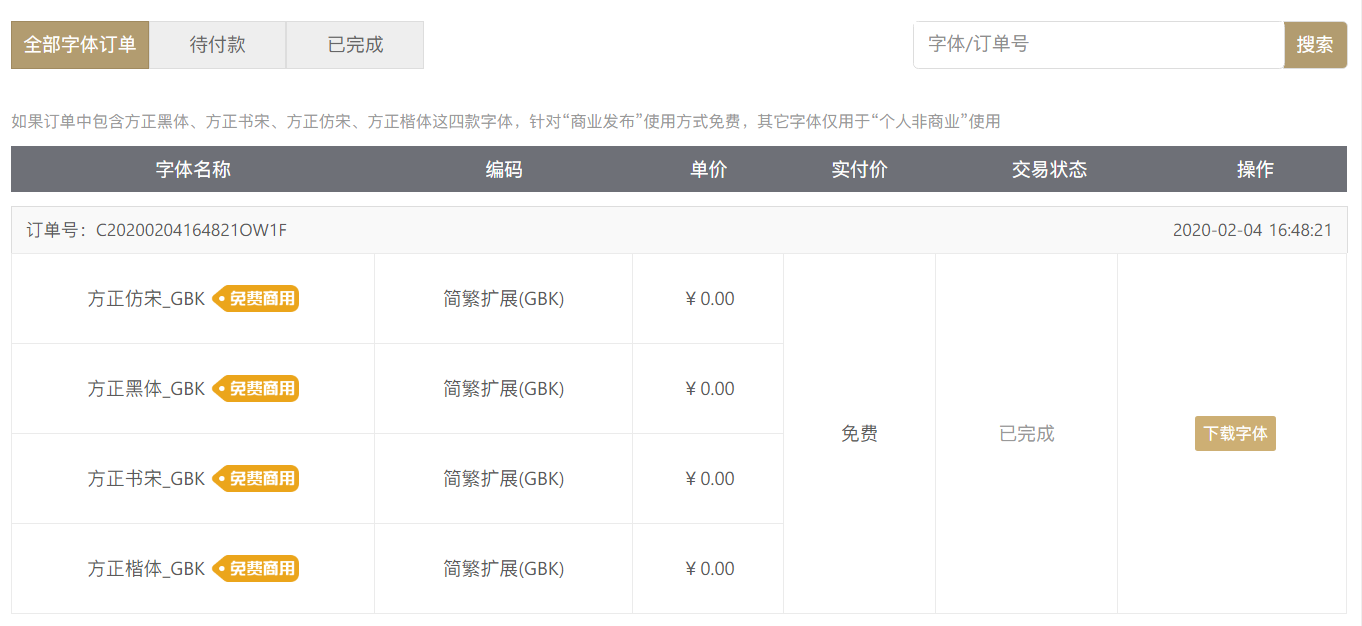
\includegraphics[width=0.9\textwidth]{founder.png}
\end{figure}

\subsection{其他中文字体}
如果你想完全自定义字体\footnote{这里仍然以方正字体为例。},你可以选择 \lstinline{chinesefont=nofont},然后在导言区设置
\begin{lstlisting}
\setCJKmainfont[BoldFont={FZHei-B01},ItalicFont={FZKai-Z03}]{FZShuSong-Z01}
\setCJKsansfont[BoldFont={FZHei-B01}]{FZKai-Z03}
\setCJKmonofont[BoldFont={FZHei-B01}]{FZFangSong-Z02}
\setCJKfamilyfont{zhsong}{FZShuSong-Z01}
\setCJKfamilyfont{zhhei}{FZHei-B01}
\setCJKfamilyfont{zhkai}[BoldFont={FZHei-B01}]{FZKai-Z03}
\setCJKfamilyfont{zhfs}[BoldFont={FZHei-B01}]{FZFangSong-Z02}
\newcommand*{\songti}{\CJKfamily{zhsong}}
\newcommand*{\heiti}{\CJKfamily{zhhei}}
\newcommand*{\kaishu}{\CJKfamily{zhkai}}
\newcommand*{\fangsong}{\CJKfamily{zhfs}}
\end{lstlisting}

\chapter{ElegantBook 写作示例}

\begin{introduction}
  \item 积分定义~\ref{def:int}
  \item Fubini 定理~\ref{thm:fubi}
  \item 最优性原理~\ref{pro:max}
  \item 柯西列性质~\ref{property:cauchy}
  \item 韦达定理
\end{introduction}

\section{Lebesgue 积分}
在前面各章做了必要的准备后,本章开始介绍新的积分.
在 Lebesgue 测度理论的基础上建立了 Lebesgue 积分,
其被积函数和积分域更一般,可以对有界函数和无界函数统一处理。
正是由于 Lebesgue 积分的这些特点,
使得 Lebesgue 积分比 Riemann 积分具有在更一般条件下的极限定理和累次积分交换积分顺序的定理,
这使得 Lebesgue 积分不仅在理论上更完善,
而且在计算上更灵活有效。

Lebesgue 积分有几种不同的定义方式。我们将采用逐步定义非负简单函数,非负可测函数和一般可测函数积分的方式。

由于现代数学的许多分支如概率论、泛函分析、调和分析等常常用到一般空间上的测度与积分理论,在本章最后一节将介绍一般的测度空间上的积分。

\subsection{积分的定义}

我们将通过三个步骤定义可测函数的积分。首先定义非负简单函数的积分。以下设 $E$ 是 $\mathcal{R}^n$ 中的可测集。

\begin{definition}[可积性] \label{def:int} 
设 $ f(x)=\sum\limits_{i=1}^{k} a_i \chi_{A_i}(x)$ 是 $E$ 上的非负简单函数,
其中 $\{A_1,A_2,\dots,A_k\}$ 是 $E$ 上的一个可测分割,
$a_1,a_2,\ldots,a_k$ 是非负实数。
定义 $f$ 在 $E$ 上的积分为 $\int_{a}^b f(x)$
\begin{equation}
   \label{inter}
   \int_{E} f dx = \sum_{i=1}^k a_i m(A_i) 
\end{equation}
一般情况下 $0 \leq \int_{E} f dx \leq \infty$。
若 $\int_{E} f dx < \infty$,
则称 $f$ 在 $E$ 上可积。
\end{definition}

一个自然的问题是,Lebesgue 积分与我们所熟悉的 Riemann 积分有什么联系和区别?在 4.4 在我们将详细讨论 Riemann 积分与 Lebesgue 积分的关系。这里只看一个简单的例子。设 $D(x)$ 是区间 $[0,1]$ 上的 Dirichlet 函数。即 $D(x)=\chi_{Q_0}(x)$,其中 $Q_0$ 表示 $[0,1]$ 中的有理数的全体。根据非负简单函数积分的定义,$D(x)$ 在 $[0,1]$ 上的 Lebesgue 积分为
\begin{equation}
   \label{inter2}
   \int_0^1 D(x)dx = \int_0^1 \chi_{Q_0} (x) dx = m(Q_0) = 0
\end{equation}
即 $D(x)$ 在 $[0,1]$ 上是 Lebesgue 可积的并且积分值为零。但 $D(x)$ 在 $[0,1]$ 上不是 Riemann 可积的。


有界变差函数是与单调函数有密切联系的一类函数。有界变差函数可以表示为两个单调递增函数之差。与单调函数一样,有界变差函数几乎处处可导。与单调函数不同,有界变差函数类对线性运算是封闭的,它们构成一线空间。练习题 \ref{exer:43} 是一个性质的证明。

\begin{exercise}\label{exer:43}
设 $f \notin\in L(\mathcal{R}^1)$,$g$ 是 $\mathcal{R}^1$ 上的有界可测函数。证明函数
\begin{equation}
   \label{ex:1}
   I(t) = \int_{\mathcal{R}^1} f(x+t)g(x)dx \quad t \in \mathcal{R}^1
\end{equation}
是 $\mathcal{R}^1$ 上的连续函数。 
\end{exercise}

\begin{solution}
即 $D(x)$ 在 $[0,1]$ 上是 Lebesgue 可积的并且积分值为零。但 $D(x)$ 在 $[0,1]$ 上不是 Riemann 可积的。
\end{solution}

\begin{proof}
即 $D(x)$ 在 $[0,1]$ 上是 Lebesgue 可积的并且积分值为零。但 $D(x)$ 在 $[0,1]$ 上不是 Riemann 可积的。
\end{proof}

\begin{theorem}[Fubini 定理] \label{thm:fubi} 
(1)若 $f(x,y)$ 是 $\mathcal{R}^p\times\mathcal{R}^q$ 上的非负可测函数,则对几乎处处的 $x\in \mathcal{R}^p$,$f(x,y)$ 作为 $y$ 的函数是 $\mathcal{R}^q$ 上的非负可测函数,$g(x)=\int_{\mathcal{R}^q}f(x,y) dy$ 是 $\mathcal{R}^p$ 上的非负可测函数。并且
\begin{equation}
   \label{eq:461}
   \int_{\mathcal{R}^p\times\mathcal{R}^q} f(x,y) dxdy=\int_{\mathcal{R}^p}\left(\int_{\mathcal{R}^q}f(x,y)dy\right)dx.
\end{equation}

(2)若 $f(x,y)$ 是 $\mathcal{R}^p\times\mathcal{R}^q$ 上的可积函数,则对几乎处处的 $x\in\mathcal{R}^p$,$f(x,y)$ 作为 $y$ 的函数是 $\mathcal{R}^q$ 上的可积函数,并且 $g(x)=\int_{\mathcal{R}^q}f(x,y) dy$ 是 $\mathcal{R}^p$ 上的可积函数。而且~\eqref{eq:461} 成立。
\end{theorem}

\begin{note}
在本模板中,引理(lemma),推论(corollary)的样式和定理~\ref{thm:fubi} 的样式一致,包括颜色,仅仅只有计数器的设置不一样。
\end{note}

我们说一个实变或者复变量的实值或者复值函数是在区间上平方可积的,如果其绝对值的平方在该区间上的积分是有限的。所有在勒贝格积分意义下平方可积的可测函数构成一个希尔伯特空间,也就是所谓的 $L^2$ 空间,几乎处处相等的函数归为同一等价类。形式上,$L^2$ 是平方可积函数的空间和几乎处处为 0 的函数空间的商空间。

\begin{proposition}[最优性原理] \label{pro:max}
如果 $u^*$ 在 $[s,T]$ 上为最优解,则 $u^*$ 在 $[s, T]$ 任意子区间都是最优解,假设区间为 $[t_0, t_1]$ 的最优解为 $u^*$ ,则 $u(t_0)=u^{*}(t_0)$,即初始条件必须还是在 $u^*$ 上。
\end{proposition}

我们知道最小二乘法可以用来处理一组数据,可以从一组测定的数据中寻求变量之间的依赖关系,这种函数关系称为经验公式。本课题将介绍最小二乘法的精确定义及如何寻求点与点之间近似成线性关系时的经验公式。假定实验测得变量之间的 $n$ 个数据,则在平面上,可以得到 $n$ 个点,这种图形称为 “散点图”,从图中可以粗略看出这些点大致散落在某直线近旁, 我们认为其近似为一线性函数,下面介绍求解步骤。

\begin{figure}[htbp]
  \centering
  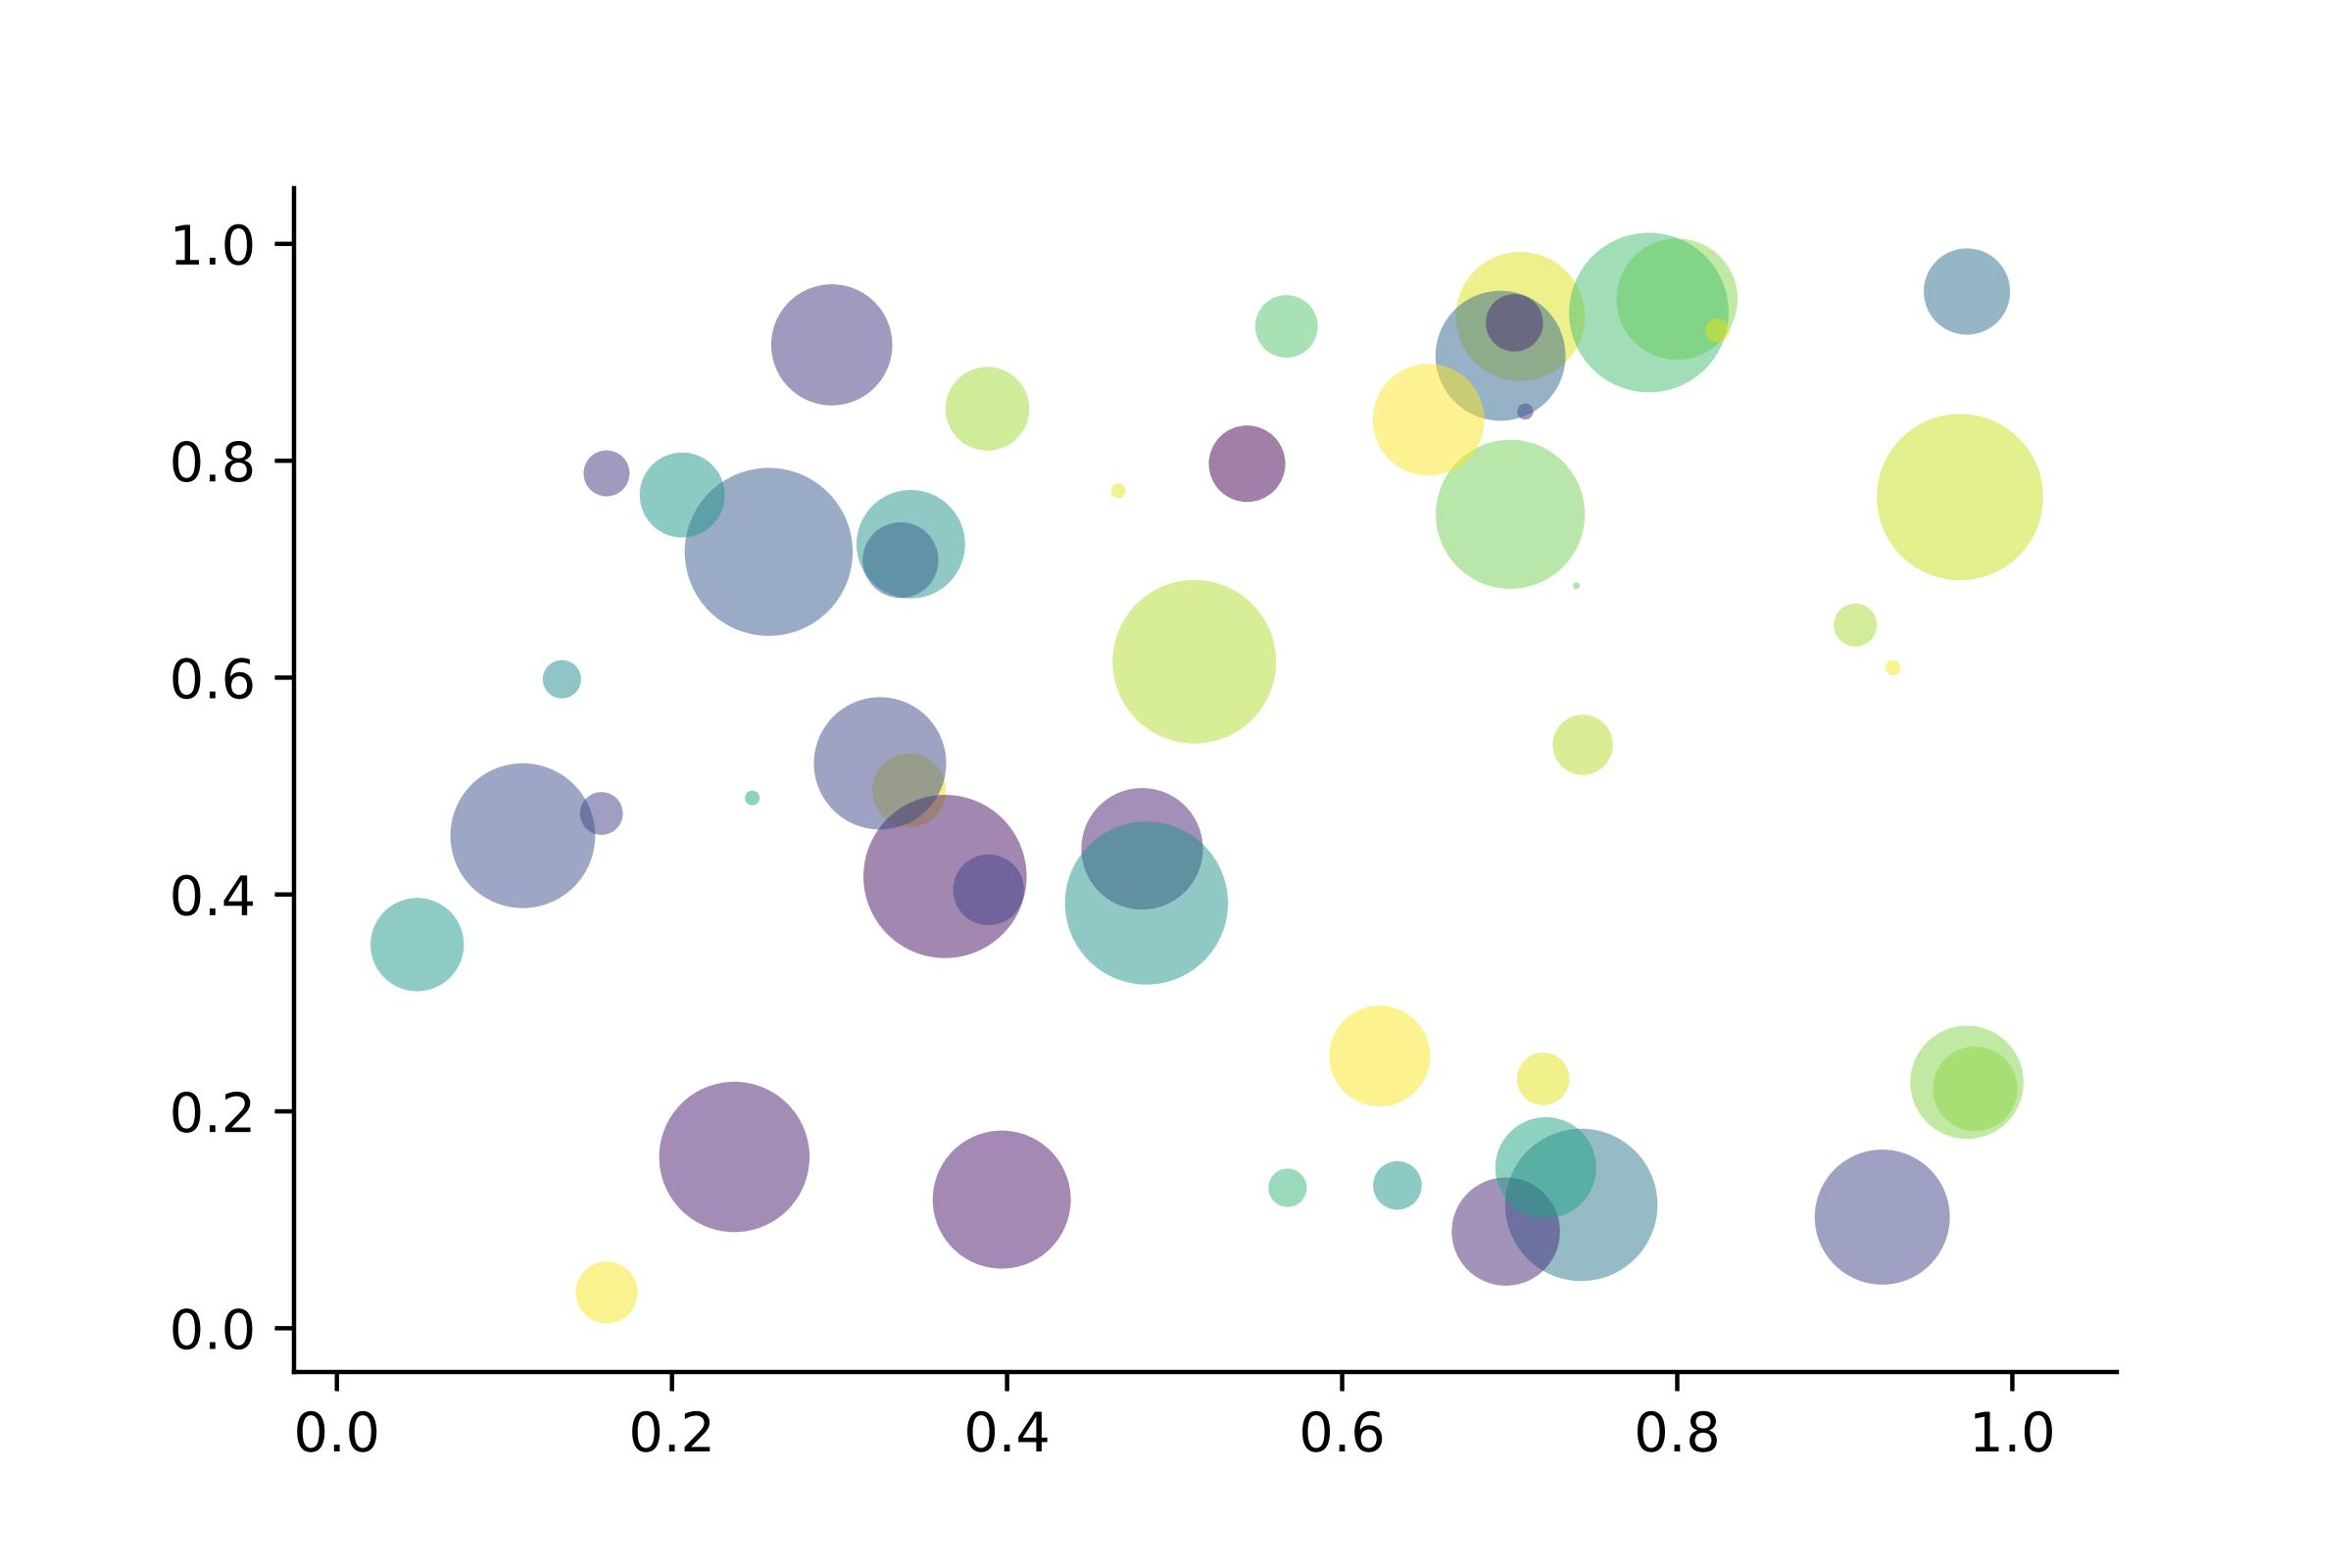
\includegraphics[width=0.6\textwidth]{scatter.jpg}
  \caption{散点图示例 $\hat{y}=a+bx$ \label{fig:scatter}}
\end{figure}

以最简单的一元线性模型来解释最小二乘法。什么是一元线性模型呢?监督学习中,如果预测的变量是离散的,我们称其为分类(如决策树,支持向量机等),如果预测的变量是连续的,我们称其为回归。回归分析中,如果只包括一个自变量和一个因变量,且二者的关系可用一条直线近似表示,这种回归分析称为一元线性回归分析。如果回归分析中包括两个或两个以上的自变量,且因变量和自变量之间是线性关系,则称为多元线性回归分析。对于二维空间线性是一条直线;对于三维空间线性是一个平面,对于多维空间线性是一个超平面。

\begin{property}\label{property:cauchy}
柯西列的性质
\begin{enumerate}
\item $\{x_k\}$ 是柯西列,则其子列 $\{x_k^i\}$ 也是柯西列。
\item $x_k\in \mathcal{R}^n$,$\rho(x,y)$ 是欧几里得空间,则柯西列收敛,$(\mathcal{R}^n,\rho)$ 空间是完备的。
\end{enumerate}
\end{property}

\begin{conclusion}
回归分析(regression analysis) 是确定两种或两种以上变量间相互依赖的定量关系的一种统计分析方法。运用十分广泛,回归分析按照涉及的变量的多少,分为一元回归和多元回归分析;按照因变量的多少,可分为简单回归分析和多重回归分析;按照自变量和因变量之间的关系类型,可分为线性回归分析和非线性回归分析。
\end{conclusion}

\begin{problemset}
\item 设 $A$ 为数域 $K$ 上的 $n$ 级矩阵。证明:如果 $K^n$ 中任意非零列向量都是 $A$ 的特征向量,则 $A$ 一定是数量矩阵。
\item 证明:不为零矩阵的幂零矩阵不能对角化。
\item 设 $A = (a_{ij})$ 是数域 $K$ 上的一个 $n$ 级上三角矩阵,证明:如果 $a_{11} = a_{22} = \cdots = a_{nn}$,并且至少有一个 $a_{kl} \not = 0 (k < l)$,则 $A$ 一定不能对角化。
\end{problemset}

\chapter{常见问题集}

我们根据用户社区反馈整理了下面一些常见的问题,用户在遇到问题时,应当首先查阅本手册和本部分的常见的问题。

\begin{enumerate}[itemsep=1.5ex]
  \item \question{有没有办法章节用“第一章,第一节,(一)”这种?}
    见前文介绍,可以使用 \lstinline{scheme=chinese} 设置。
  \item \question{大佬,我想把正文字体改为亮色,背景色改为黑灰色。}
    页面颜色可以使用 \lstinline{\pagecolor} 命令设置,文本命令可以参考\href{https://tex.stackexchange.com/questions/278544/xcolor-what-is-the-equivalent-of-default-text-color}{这里}进行设置。
  \item \question{\lstinline{! LaTeX Error: Unknown option 'scheme=plain' for package 'ctex'.}}
    你用的 C\TeX{} 套装吧?这个里面的 \lstinline{ctex} 宏包已经是已经是 10 年前的了,与本模板使用的 \lstinline{ctex} 宏集有很大区别。不建议 C\TeX{} 套装了,请卸载并安装 \TeX{} Live 2022。
  \item \question{我该使用什么版本?}
    请务必使用\href{https://github.com/ElegantLaTeX/ElegantBook/releases}{最新正式发行版},发行版间不定期可能会有更新(修复 bug 或者改进之类),如果你在使用过程中没有遇到问题,不需要每次更新\href{https://github.com/ElegantLaTeX/ElegantBook/archive/master.zip}{最新版},但是在发行版更新之后,请尽可能使用最新版(发行版)!最新发行版可以在 GitHub 或者 \TeX{} Live 2021 内获取。
  \item \question{我该使用什么编辑器?}
    你可以使用 \TeX{} Live 2021 自带的编辑器 \TeX{}works 或者使用 \TeX{}studio,\TeX works 的自动补全,你可以参考我们的总结 \href{https://github.com/EthanDeng/texworks-autocomplete}{\TeX works 自动补全}。推荐使用 \TeX{} Live 2021 + \TeX{}studio。我自己用 VS Code 和 Sublime Text,相关的配置说明,请参考 \href{https://github.com/EthanDeng/vscode-latex}{\LaTeX{} 编译环境配置:Visual Studio Code 配置简介} 和 \href{https://github.com/EthanDeng/sublime-text-latex}{Sublime Text 搭建 \LaTeX{} 编写环境}。
  \item \question{您好,我们想用您的 ElegantBook 模板写一本书。关于机器学习的教材,希望获得您的授权,谢谢您的宝贵时间。}
    模板的使用修改都是自由的,你们声明模板来源以及模板地址(GitHub 地址)即可,其他未尽事宜按照开源协议 LPPL-1.3c。做好之后,如果方便的话,可以给我们一个链接,我把你们的教材放在 Elegant\LaTeX{} 用户作品集里。
  \item \question{请问交叉引用是什么?}
    本群和本模板适合有一定 \LaTeX{} 基础的用户使用,新手请先学习 \LaTeX{} 的基础,理解各种概念,否则你将寸步难行。
  \item \question{代码高亮环境能用其他语言吗?}
    可以的,ElegantBook 模板用的是 \lstinline{listings} 宏包,你可以在环境(\lstinline{lstlisting})之后加上语言(比如 Python 使用 \lstinline{language=Python} 选项),全局语言修改请使用 \lstinline{lstset} 命令,更多信息请参考宏包文档。
  \item \question{群主,什么时候出 Beamer 的模板(主题),ElegantSlide 或者 ElegantBeamer?}
    由于 Beamer 中有一个很优秀的主题 \href{https://github.com/matze/mtheme}{Metropolis}。后续确定不会再出任何主题/模板,请大家根据需要修改已有主题。
\end{enumerate}

\chapter{版本更新历史}

根据用户的反馈,我们不断修正和完善模板。由于 3.00 之前版本与现在版本差异非常大,在此不列出 3.00 之前的更新内容。

\datechange{2022/12/31}{版本 4.5} \textcolor{red}{\bfseries 停止维护!}

\datechange{2022/08/17}{版本 4.5 pre}
\begin{change}
  \item \textbf{重要改动}:提供了一个新的文档类选项 \lstinline|usesamecnt|,可以使全局的定理类环境使用同一个计数器。
  \item \textbf{重要改动}:修改了 \lstinline|\elegantnewtheorem| 命令,使其有第五个(可选)参数。
\end{change}

\datechange{2022/08/15}{版本 4.4 正式发布。}

\begin{change}
  \item \textbf{重要改动}:提供了一个定义定理类环境的命令 \lstinline|\elegantnewtheorem|;
  \item \textbf{重要改动}:为所有内置定理类环境提供了带星号的版本,带星号的定理类环境不会编号,修复 \href{https://github.com/ElegantLaTeX/ElegantBook/issues/167}{issue: \#167};
  \item \textbf{重要改动}:在 \lstinline{scheme=chinese} 下将目录中的“第 1 章”修改为“第一章”;
  \item 将 TeX Gyre Termes 改为 TeX Gyre TermesX,使英文部分字形与 newtx 系列宏包更相近;
  \item 重写了内置定理类环境的实现方法,修复了一些 bug,由于修改部分较大,如果引入了新的 bug,请及时在 QQ 群或 \href{https://github.com/ElegantLaTeX}{Github} 上进行反馈;
  \item 删除 Gitee 仓库地址,恢复 GitHub 提交(pull requests);
  \item 将参考文献命令添加到导言区,使编辑器能够对参考文献自动补全。
\end{change}

\datechange{2022/04/09}{版本 4.3 正式发布。}

\begin{change}
  \item 放弃 newtx 系列宏包的设置,改用 TeX Gyre Termes,并设置其他字体;
  \item 修改定理类环境内部字体设置,修复环境内部中文无法加粗问题;
  \item 增加定理类环境的计数器选项 \lstinline{thmcnt},可选 \lstinline{chapter} 和 \lstinline{section};
  \item 增加 \lstinline{bibend} 选项,可选 \lstinline{bibend=biber}(默认)和 \lstinline{bibend=bibtex}。
\end{change}



\datechange{2022/03/08}{版本 4.2 正式发布。}

\begin{change}
  \item 对于 newtx 系列宏包更新导致的字体 bug 的修复;
  \item 修缮目录格式,为了达到这个目的,重新改写 \lstinline{\chaptername} 的重定义语句;
  \item 增加日语 \lstinline{lang=jp} 设定。
  \item 这个版本为一个临时性版本,在 \TeX Live 2022 发布之后,将尽快发布 4.3 版本,由于对于中文的改动比较大,可能会出现预期之外的 bug,有问题可以在 QQ 群或者 Github 反馈。
\end{change}


\datechange{2021/05/02}{版本 4.1 正式发布。}

\begin{change}
  \item \textbf{重要改动}:由原先的 \hologo{BibTeX} 改为 biblatex 编译方式(后端为 \lstinline{biber}),请注意两者之间的差异;
  \item \textbf{重要改进}:修改对于定理写法兼容方式,提高数学公式代码的兼容性;
  \item 页面设置改动,默认页面更宽;方便书写和阅读;
  \item 支持目录文字以及页码跳转;
  \item 不再维护 \hologo{pdfLaTeX} 中文支持方式,请务必使用 \hologo{XeLaTeX} 编译中文文稿。
  \item 增加多个语言选项,法语 \lstinline{lang=fr}、荷兰语 \lstinline{lang=nl}、匈牙利语 \lstinline{lang=hu}、西班牙语 \lstinline{lang=es}、蒙古语 \lstinline{lang=mn} 等。
\end{change}


\datechange{2020/04/12}{版本 3.11 正式发布,\textcolor{red}{此版本为 3.x 最后版本。}}

\begin{change}
  \item \textbf{重要修正}:修复因为 \lstinline{gbt7714} 宏包更新导致的 \lstinline{natbib option clash} 错误;
  \item 由于 \lstinline{pgfornament} 宏包未被 \TeX{} Live 2020 收录,因此删除 base 相关的内容;
  \item 修复部分环境的空格问题;
  \item 增加了意大利语言选项 \lstinline{lang=it}。
\end{change}


\datechange{2020/02/10}{版本 3.10 正式发布}

\begin{change}
  \item 增加数学字体选项 \lstinline{math},可选项为 \lstinline{newtx} 和 \lstinline{cm}。\\
  \textbf{重要提示}:原先通过 \lstinline{newtxmath} 宏包设置的数学字体改为 \LaTeX{} 默认数学字体,如果需要保持原来的字体,需要显式声明数学字体(\lstinline{math=newtx});
  \item 新增中文字体选项 \lstinline{chinesefont},可选项为 \lstinline{ctexfont}、\lstinline{founder} 和 \lstinline{nofont}。
  \item 将封面作者信息设置为可选,并且增加自定义信息命令 \lstinline{\bioinfo};
  \item 在说明文档中增加版本历史,新增 \lstinline{\datechange} 命令和 \lstinline{change} 环境;
  \item 增加汉化章节选项 \lstinline{scheme},可选项为汉化 \lstinline{chinese};
  \item 由于 \lstinline{\lvert} 问题已经修复,重新调整 \lstinline{ctex} 宏包和 \lstinline{amsmath} 宏包位置。
  \item 修改页眉设置,去除了 \lstinline{\lastpage} 以避免 page anchor 问题,加入 \lstinline{\frontmatter}。
  \item 修改参考文献选项 \lstinline{cite},可选项为数字 \lstinline{numbers}、 作者-年份 \lstinline{authoryear} 以及上标 \lstinline{super}。
  \item 新增参考文献样式选项 \lstinline{bibstyle},并将英文模式下参考文献样式 \lstinline{apalike} 设置为默认值,中文仍然使用 \lstinline{gbt7714} 宏包设置。
\end{change}

\datechange{2019/08/18}{版本 3.09 正式发布}

\begin{change}
  \item \lstinline{\elegantpar} 存在 bug,删除 \lstinline{\elegantpar} 命令,建议用户改用 \lstinline{\marginnote} 和 \lstinline{\marginpar} 旁注命令。
  \item 积分操作符统一更改为 \lstinline{esint} 宏包设置;
  \item 新增目录选项 \lstinline{toc},可选项为单栏 \lstinline{onecol} 和双栏 \lstinline{twocol};
  \item 手动增加参考文献选项 \lstinline{cite},可选项为上标形式 \lstinline{super};
  \item 修正章节习题(\lstinline{problemset})环境。
\end{change}

\datechange{2019/05/28}{版本 3.08 正式发布}

\begin{change}
  \item 修复 \lstinline{\part} 命令。
  \item 引入 Note 模板中的 \lstinline{pad} 选项 \lstinline{device=pad}。
  \item 数学字体加入 \lstinline{mtpro2} 可选项 \lstinline{math=mtpro2},使用免费的 \lstinline{lite} 子集。
  \item 将参考文献默认显示方式 \lstinline{authoyear} 改为 \lstinline{numbers}。
  \item 引入旁注命令 \lstinline{\marginpar}(测试)。
  \item 新增章节摘要环境 \lstinline{introduction}。
  \item 新增章节习题环境 \lstinline{problemset}。
  \item 将 \lstinline{\equote} 重命名为 \lstinline{\extrainfo}。
  \item 完善说明文档,增加致谢部分。
\end{change}

\datechange{2019/04/15}{版本 3.07 正式发布}

\begin{change}
  \item 删除中英文自定义字体总设置。
  \item 新增颜色主题,并将原绿色默认主题设置为蓝色 \lstinline{color=blue}。
  \item 引入隐藏装饰图案选项 \lstinline{base},可选项有显示 \lstinline{show} 和隐藏 \lstinline{hide}。
  \item 新增定理模式 \lstinline{mode},可选项有简单模式 \lstinline{simple} 和炫彩模式 \lstinline{fancy}。
  \item 新增隐藏证明、答案等环境的选项 \lstinline{result=noanswer}。
\end{change}

\datechange{2019/02/25}{版本 3.06 正式发布}

\begin{change}
  \item 删除水印。
  \item 新封面,新装饰图案。
  \item 添加引言使用说明。
  \item 修复双面 \lstinline{twoside}。
  \item 美化列表环境。
  \item 增加 \lstinline{\subsubsection} 的设置。
  \item 将模板拆分成中英文语言模式。
  \item 使用 \lstinline{lstlisting} 添加代码高亮。
  \item 增加定理类环境使用说明。
\end{change}

\datechange{2019/01/22}{版本 3.05 正式发布}

\begin{change}
  \item 添加 \lstinline{xeCJK} 宏包中文支持方案。
  \item 修复模板之前对 Ti\textit{k}Z 单位的改动。
  \item 更新 logo 图。
\end{change}

\datechange{2019/01/15}{版本 3.04 正式发布}

\begin{change}
  \item 格式化模板代码。
  \item 增加 \lstinline{\equote} 命令。
  \item 修改 \lstinline{\date}。
\end{change}

\datechange{2019/01/08}{版本 3.03 正式发布}

\begin{change}
  \item 修复附录章节显示问题。
  \item 小幅优化封面代码。
\end{change}

\datechange{2018/12/31}{版本 3.02 正式发布}

\begin{change}
  \item 修复名字系列命令自定义格式时出现的空格问题,比如 \lstinline{\listfigurename}。
  \item 英文定理类名字改为中文名。
  \item 英文结构名改为中文。
\end{change}

\datechange{2018/12/16}{版本 3.01 正式发布}

\begin{change}
  \item 调整 \lstinline{ctex} 宏包。
  \item 说明文档增加更新内容。
\end{change}

\datechange{2018/12/06}{版本 3.00 正式发布}

\begin{change}
  \item 删除 \lstinline{mathpazo} 数学字体选项。
  \item 添加邮箱命令 \lstinline{\mailto}。
  \item 修改英文字体为 \lstinline{newtx} 系列,另外大型操作符号维持 cm 字体。
  \item 中文字体改用 \lstinline{ctex} 宏包自动设置。
  \item 删除 \lstinline{xeCJK} 字体设置,原因是不同系统字体不方便统一。
  \item 定理换用 \lstinline{tcolorbox} 宏包定义,并基本维持原有的定理样式,优化显示效果,支持跨页;定理类名字重命名,如 etheorem 改为 theorem 等等。
  \item 删去自定义的缩进命令 \lstinline{\Eindent}。
  \item 添加参考文献宏包 \lstinline{natbib}。
  \item 颜色名字重命名。
\end{change}

\nocite{*}




\printbibliography[heading=bibintoc, title=\ebibname]
\appendix

\chapter{基本数学工具}


本附录包括了计量经济学中用到的一些基本数学,我们扼要论述了求和算子的各种性质,研究了线性和某些非线性方程的性质,并复习了比例和百分数。我们还介绍了一些在应用计量经济学中常见的特殊函数,包括二次函数和自然对数,前 4 节只要求基本的代数技巧,第 5 节则对微分学进行了简要回顾;虽然要理解本书的大部分内容,微积分并非必需,但在一些章末附录和第 3 篇某些高深专题中,我们还是用到了微积分。

\section{求和算子与描述统计量}

\textbf{求和算子} 是用以表达多个数求和运算的一个缩略符号,它在统计学和计量经济学分析中扮演着重要作用。如果 $\{x_i: i=1, 2, \ldots, n\}$ 表示 $n$ 个数的一个序列,那么我们就把这 $n$ 个数的和写为:

\begin{equation}
\sum_{i=1}^n x_i \equiv x_1 + x_2 +\cdots + x_n
\end{equation}



\end{document}
